%%=============================================================================
%% chapters/chapter6.tex — Experiments and Results (final-defense version)
%%=============================================================================
\chapter{Experiments and Results}
\label{ch:experiments}
This chapter reports the experimental design and results for the three parts
of the framework.\footnote{The results of this chapter are reported in the author's publications~\cite{iccas2026,kim2026sensors,kim2026ictc,kim2026electronics,raaicon2026}; tables and figures are reproduced from them with the source indicated.} Section~\ref{sec:setup} describes the platforms, scenes,
ground-truth protocol, and metrics. Section~\ref{sec:exp-mapping} evaluates
the automated mapping subsystem of Chapter~\ref{ch:mapping} in a controlled
simulation ablation, on hardware, and through survey-grade registration.
Sections~\ref{sec:exp-seg}--\ref{sec:exp-ablation} evaluate the semantic
modeling subsystem of Chapter~\ref{ch:semantic}: segmentation repeatability
and backbone selection, multi-view verification and escalation, the owner
audit and corrective feedback, knowledge-grounded querying, incremental update,
an end-to-end replay, and ablations including a cross-floor stress scene.
Sections~\ref{sec:exp-twin} and~\ref{sec:exp-missions} evaluate the digital
twin and the semantic mission execution of Chapter~\ref{ch:validation} in
simulation and on the physical robot. Section~\ref{sec:exp-summary} maps the
results back to the research objectives.

\section{Experimental Setup}
\label{sec:setup}

\subsection{Platforms and Software Stack}
\label{subsec:platforms}

The mapping subsystem is implemented as a set of decoupled ROS~2 (Jazzy) nodes.
A mobile base builds a 2D occupancy map online with Cartographer
SLAM~\cite{hess2016}; the frontier explorer~\cite{guler2024} selects goals and
drives the robot through the Nav2 navigation stack~\cite{macenski2020marathon}
using a sampling-based model-predictive path integral
controller~\cite{williams2016}; and the stop-and-scan sequencer applies the
placement policy of Chapter~\ref{ch:mapping}. Nav2 plans on an inflated
costmap, so every path and every scan candidate keeps the robot footprint clear
of obstacles by the inflation margin (0.70~m inflation radius with a 0.22~m
robot radius in all reported runs). The target stationary sensor is a Leica
BLK360~G1 terrestrial laser scanner; a driver connects to the physical device
over Wi-Fi and executes its full-dome scan workflow.

Two mobile platforms are used. \textbf{RedBOT04} (Figure~\ref{fig:redbot}) is
the scan platform: a four-wheeled skid-steer base (footprint $71\times49$~cm)
driven by four BLDC gearmotors, with an industrial PC main controller and an
STM32 sub-controller; a YDLiDAR TG30 provides the 2D scan for SLAM and
navigation, and the BLK360 is mounted on the deck about 0.5~m above the
floor---lower than a typical 1.5--1.8~m tripod setup, so low furniture casts
longer horizontal shadows than in a manual survey. \textbf{AMMR} is the
spatial-operation robot of Chapter~\ref{ch:validation}: a swerve-drive mobile
manipulator (body $1.24\times0.79$~m) running its own AMCL localization and
Nav2 stack on an independently built map. For the controlled coverage
evaluation, a TurtleBot3 Waffle is the mobile base in
Gazebo~\cite{koenig2004gazebo}, and the physical scanner is replaced by a mock
scanner node that reproduces the BLK360 capture-and-download timing and its
failure-and-retry behavior. The semantic modeling pipeline runs on a desktop
workstation (AMD Ryzen~9 9900X, 32~GB RAM, NVIDIA RTX PRO 4000 Blackwell
24~GB), which also hosts Isaac Sim~5.1 for the twin.

\begin{figure}[!htb]
\centering
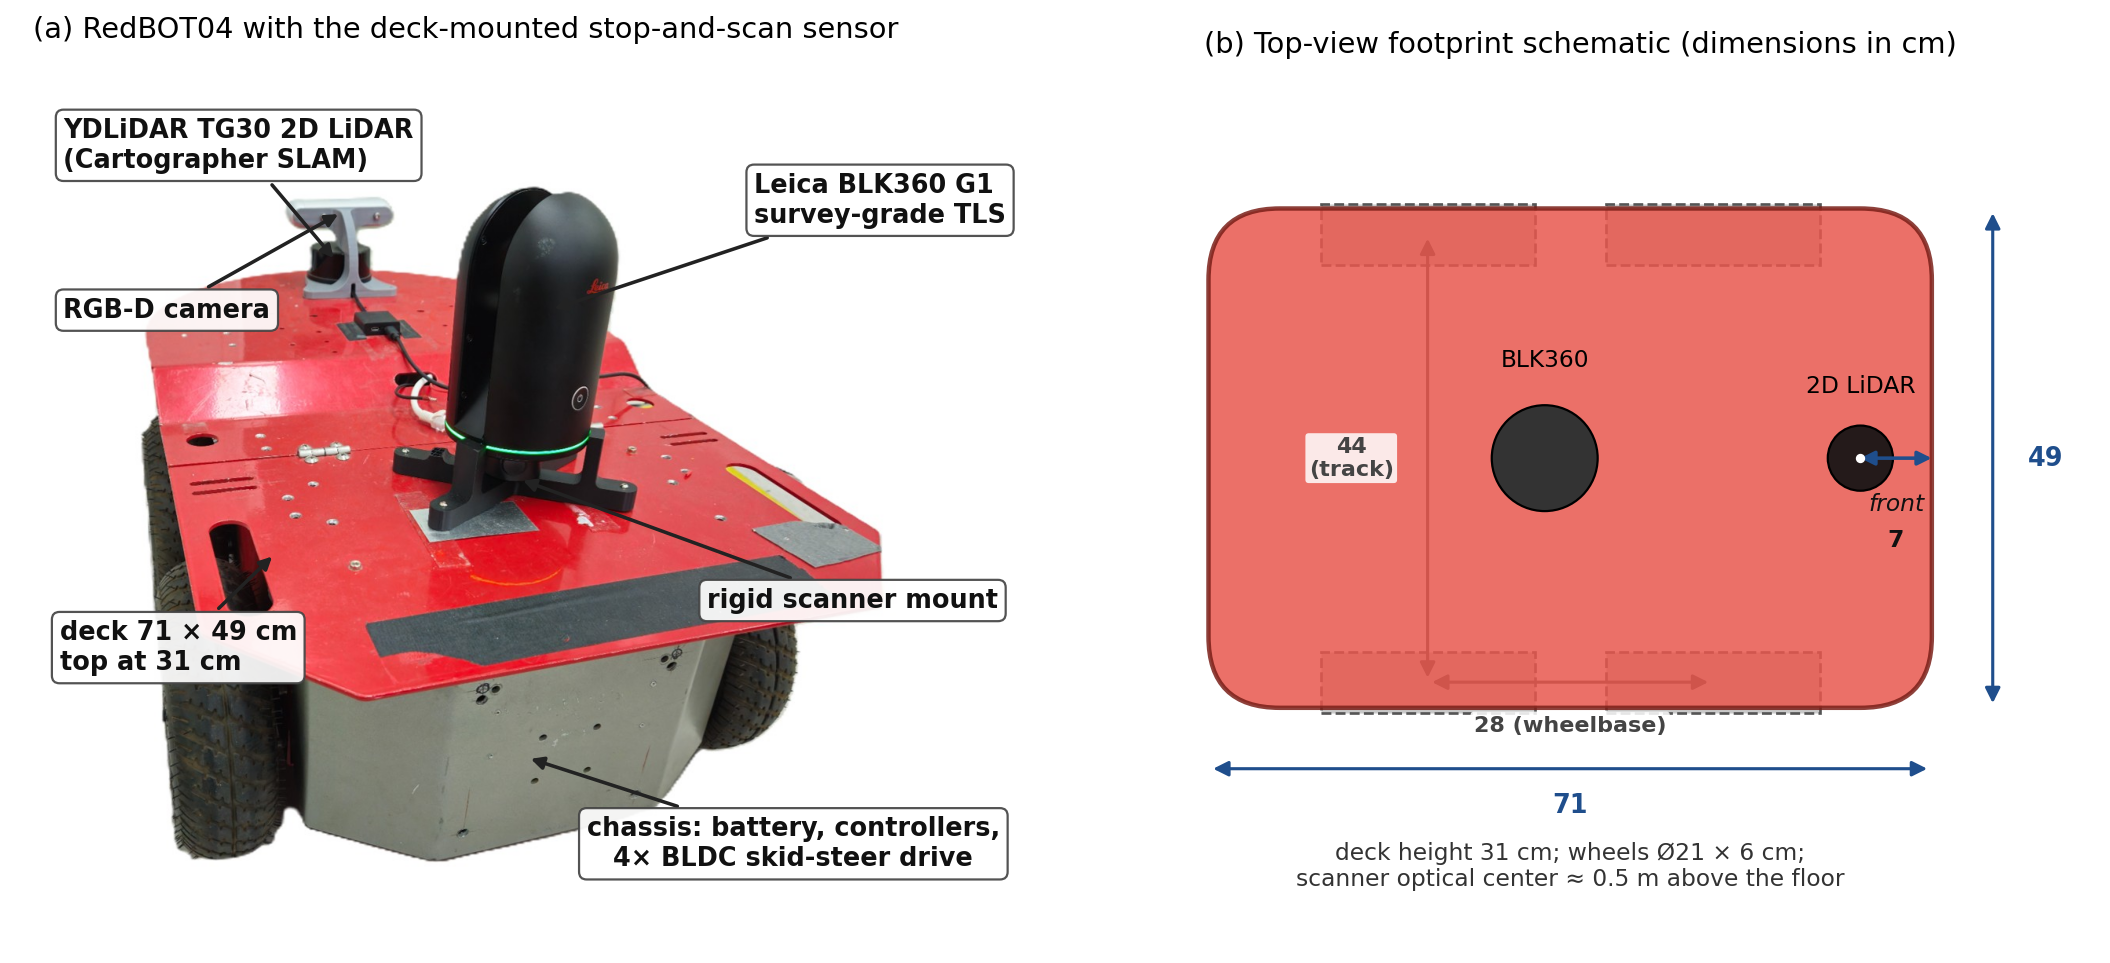
\includegraphics[width=0.9\linewidth]{figures/sen_fig9_redbot04_platform_annot.png}
\caption{RedBOT04 mobile scan platform. (a)~Annotated view with the
deck-mounted Leica BLK360~G1; (b)~top-view footprint schematic with the
principal dimensions (cm).}
\label{fig:redbot}
\end{figure}

\subsection{Environments, Scenes, and Epochs}
\label{subsec:scenes}

Two simulated indoor worlds are used for the mapping ablation. The
single-room world is generated from a real BLK360 scan of the test room,
converted to a 2D occupancy grid and extruded into a Gazebo world, so the
simulated geometry reflects the real environment
(Figure~\ref{fig:gazebo}). The multi-room world extends it with two interior
partitions and offset doorways, producing three rooms with mutual occlusion.
The physical environment for the hardware experiments and for all semantic
modeling is an \textbf{industrial test room} on the fourth floor of the
company building: an open exhibition and staging space of approximately
$13\times9$~m with a flat reflective floor, a display wall of monitors and
product panels, freestanding equipment cases, robots, and furniture that create
genuine self-occlusion (Figure~\ref{fig:testroom}); its mapped free space
spans about 105~m$^2$ on the reference map. The room combines surface types
known to stress laser-scan-based reconstruction (glass windows, dark
light-absorbing equipment, reflective flooring), it is the actual deployment
environment of the AMMR, and it allows controlled, repeatable access for the
tape-measured ground-truth campaign and the on-robot experiments.

\begin{figure}[!htb]
  \centering
  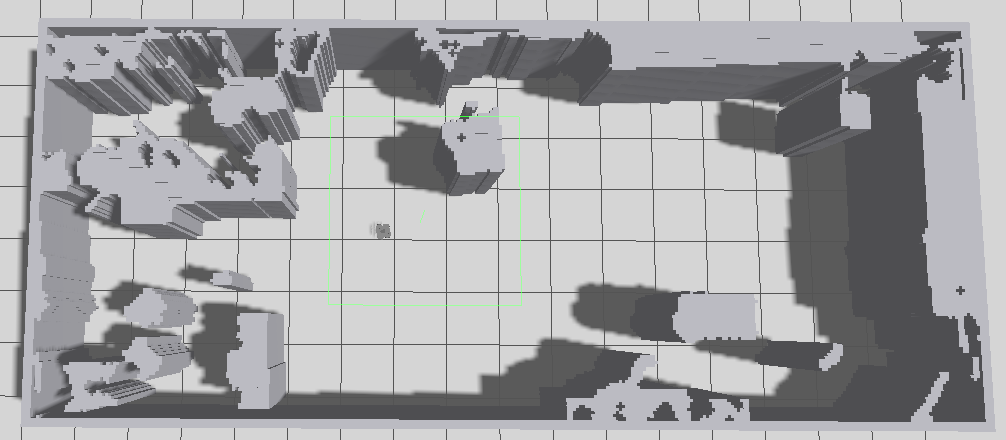
\includegraphics[width=0.85\textwidth]{figures/fig6_gazebo.png}
  \caption{The physics-based Gazebo simulation environment, built by extruding
  the 2D occupancy projection of a real survey-grade scan of the test room into
  a 3D world; the differential-drive platform explores it under the
  Cartographer/Nav2 stack.}
  \label{fig:gazebo}
\end{figure}

\begin{figure}[!htb]
\centering
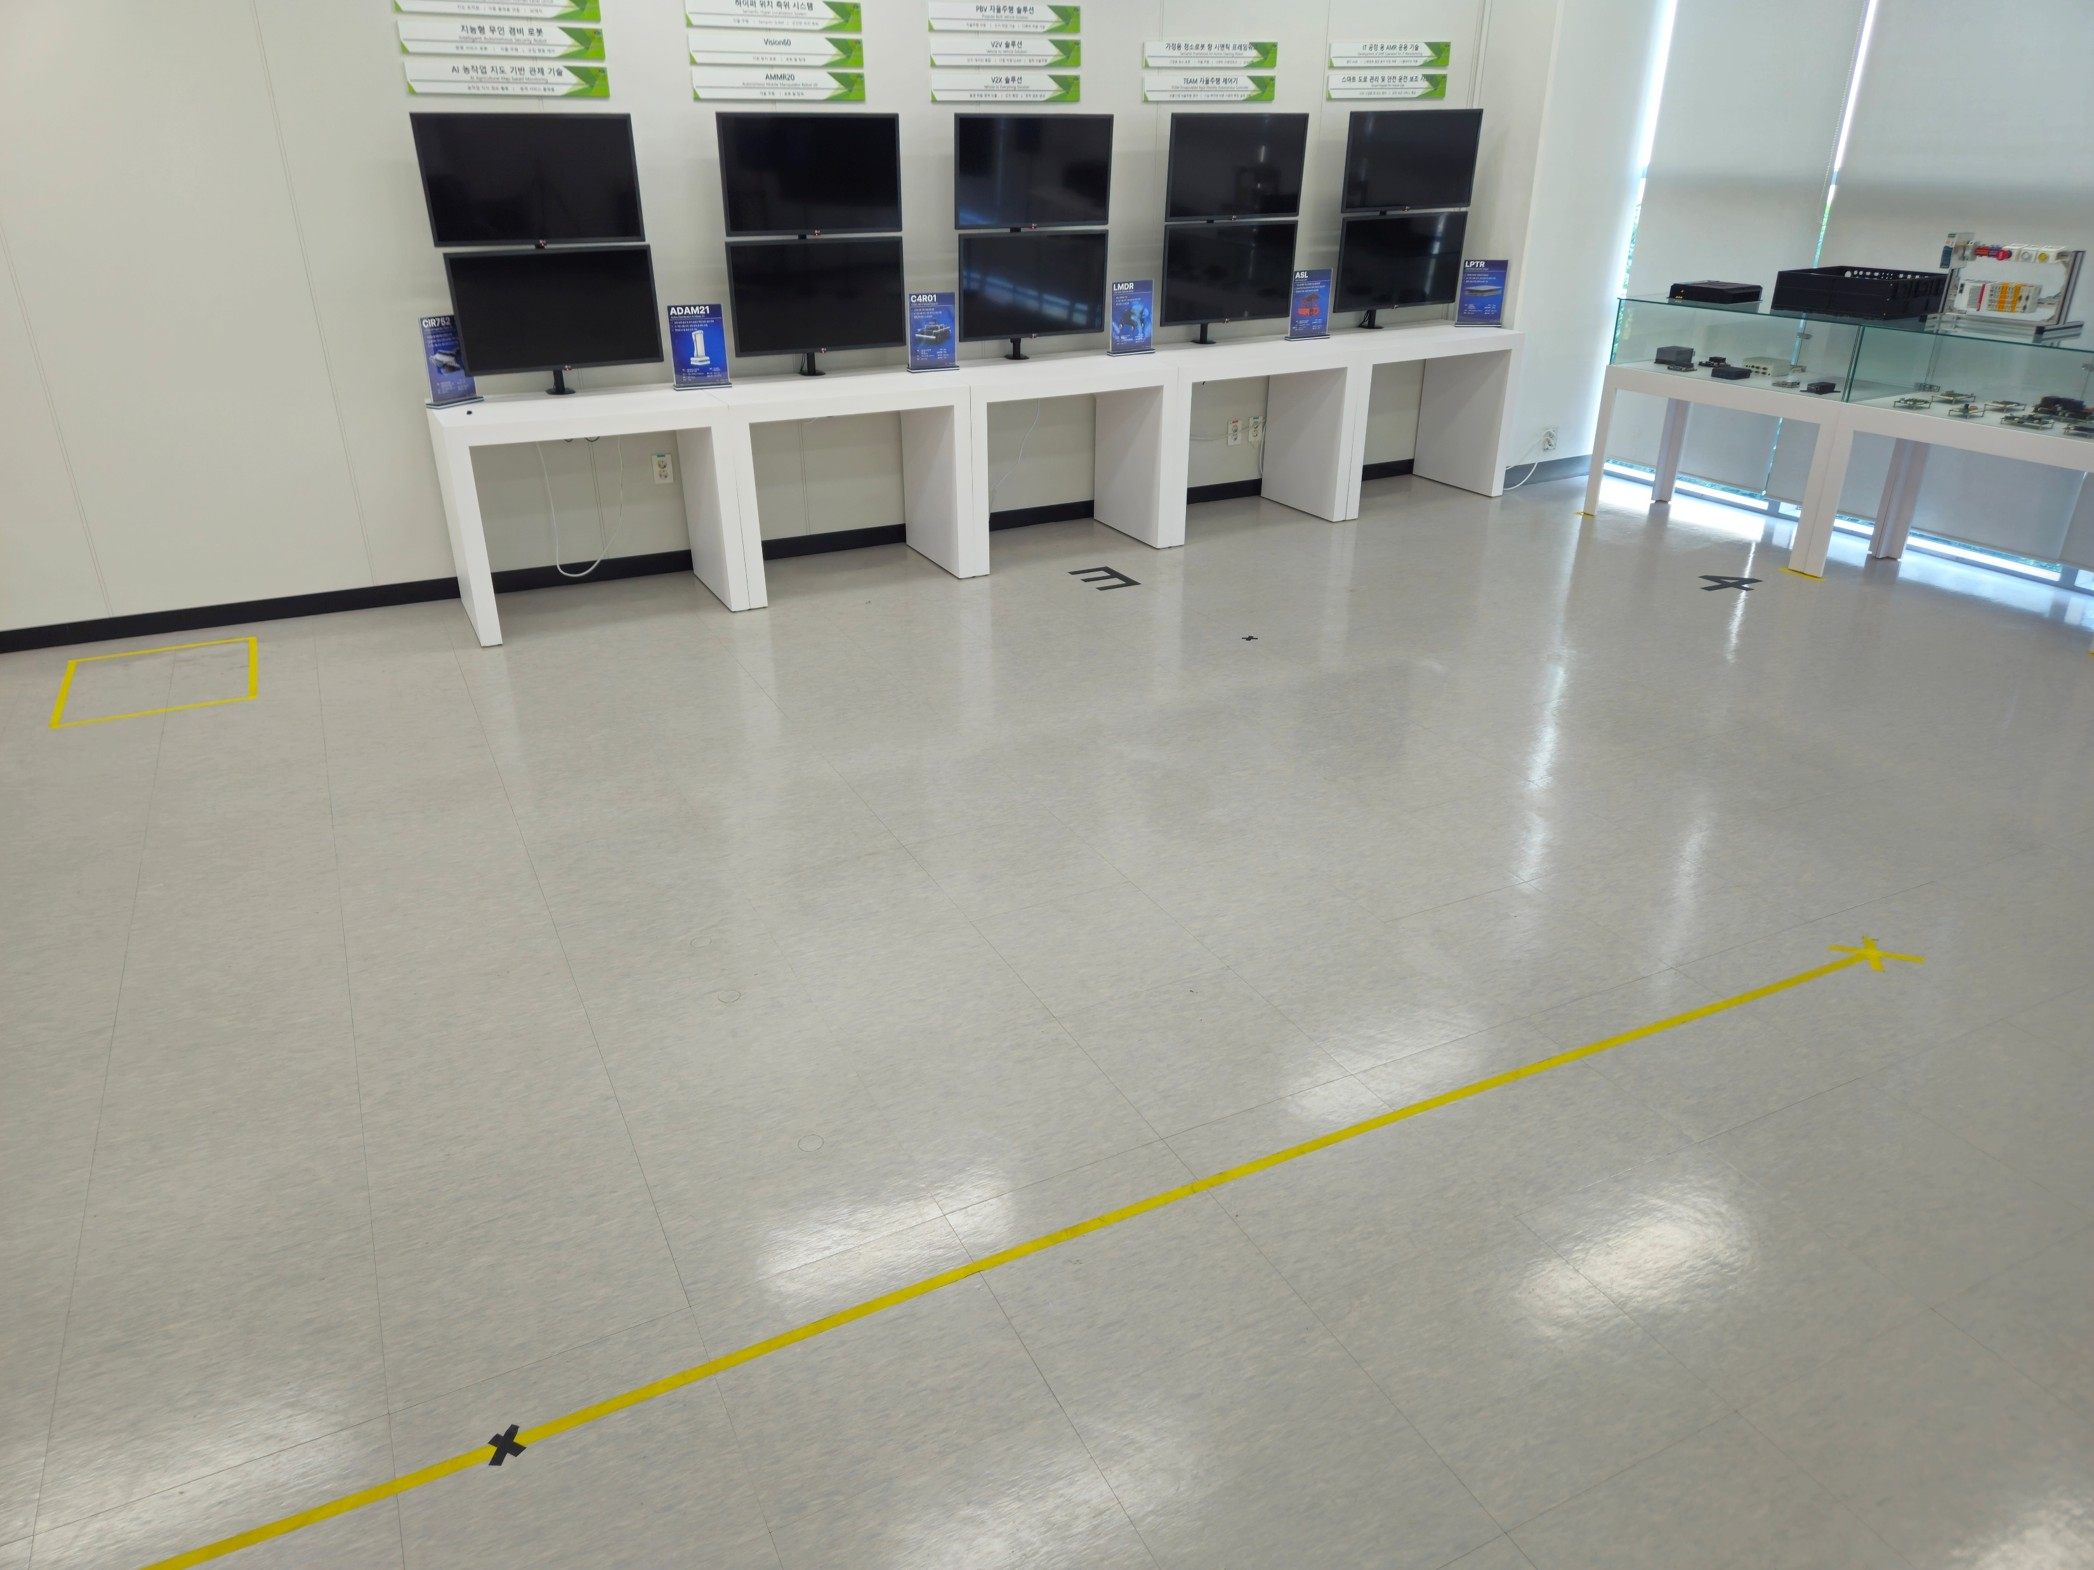
\includegraphics[width=0.9\linewidth]{figures/sen_fig10_testroom.jpg}
\caption{Physical industrial test room used for the hardware experiments and
for all semantic modeling scenes.}
\label{fig:testroom}
\end{figure}

For semantic modeling, the same room is observed across three scan epochs of
its working life, a property exploited deliberately (Table~\ref{tab:scenes},
Figure~\ref{fig:photos}). The \emph{showroom} epoch (T1, June 2026) captures
the room in an exhibition configuration, scanned manually with the door open.
The \emph{robot hall} epoch (T2, July 2026) captures the same room reorganized
as a robot test hall, scanned by autonomous visibility-driven exploration. A
third epoch (T3, late July 2026) adds a controlled-change re-scan at 99.6\%
LOS coverage. Because the two primary epochs differ in layout, furnishing, and
scan modality, they function as independent scenes for per-epoch evaluation
while enabling a real multi-epoch update study. A separate scene---a carpeted
\emph{cafeteria} with sofa booths and vending machines on the eighth floor of
the same building, scanned in August 2026 (57~M points, 28 clusters)---is held
out of the main campaign and used only as a cross-floor, out-of-vocabulary
stress case. Table~\ref{tab:sampleflow} connects every cluster set used in
this chapter to its derivation stage.

\begin{figure}[!htb]
\centering
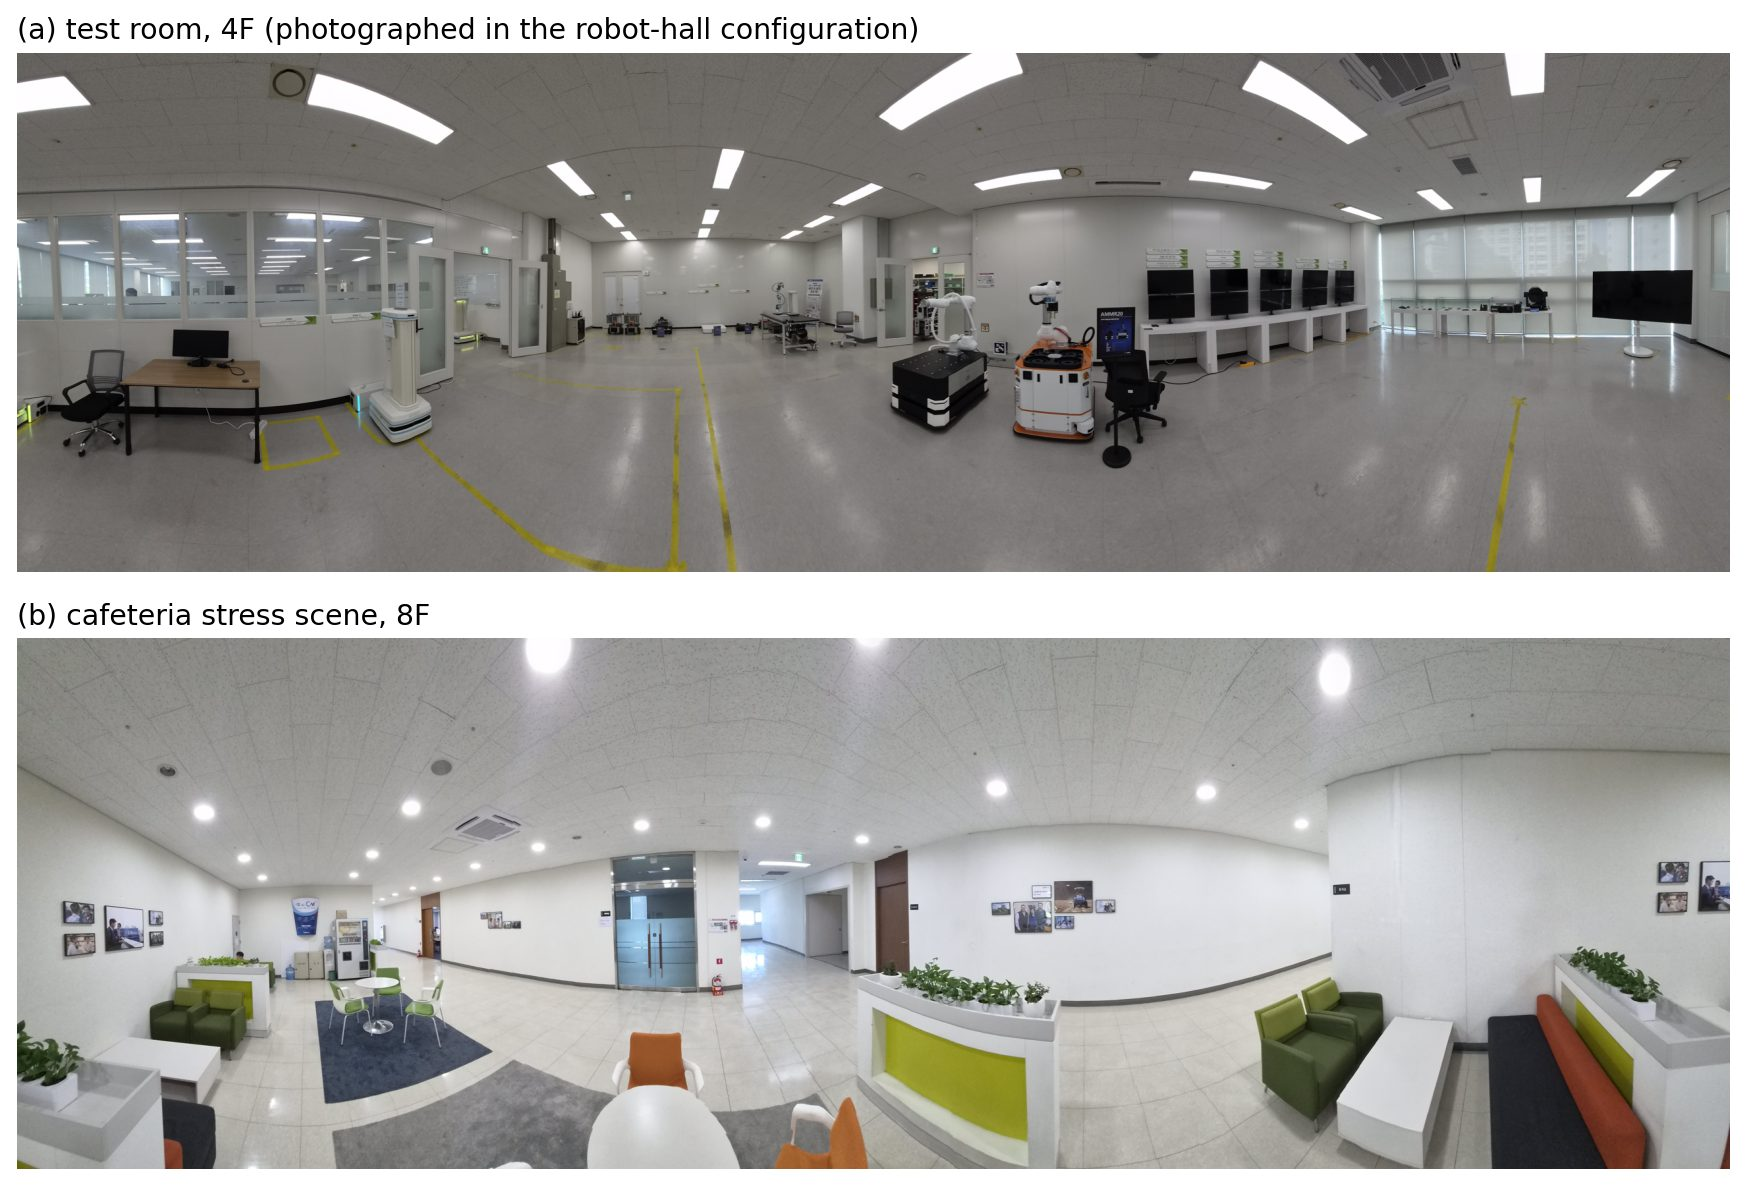
\includegraphics[width=\linewidth]{figures/ele_fig18_scene_photos.jpg}
\caption{The two semantic-modeling sites. (a)~The 4F test room in its
robot-hall configuration (T1 is an earlier furnishing of the same room;
visible: the AMMR platforms, the wall-mounted monitor bank, and a disinfection
robot). (b)~The 8F cafeteria stress scene: fabric sofas, planter partitions,
the vending row, and the brown door recovered by escalation on full-resolution
renders.}
\label{fig:photos}
\end{figure}

\begin{table}[htbp]
\centering
\caption{Scene statistics (deterministic detection sets after
structure-remnant filtering). T1 semantic processing starts from a manually
wall-removed export (4.9~M points) of the 46.3~M-point raw scan.}
\label{tab:scenes}
\small
\begin{tabularx}{\textwidth}{X c c c}
\toprule
 & \textbf{Showroom (T1)} & \textbf{Robot hall (T2)} & \textbf{Re-scan (T3)} \\
\midrule
Scan mode & manual, 1 setup & exploration & exploration, 6 setups \\
Raw points & 46.3M & 68.6M & 70.2M \\
Clean cloud (post-removal) & --- & 267K & 294K \\
Objects (filtered) & 38 & 81 & 79 \\
Room-scoped & 38 & 55 & 41 \\
Removed planes & 10 & 10 & 10 \\
\bottomrule
\end{tabularx}
\end{table}

\begin{table}[htbp]
\centering
\caption{Evaluation-set lineage: how every cluster set used in this chapter
derives from its scan ($\dagger$: grounded only in the experiment log;
``conf.''\,=\,ground-truth confirmed).}
\label{tab:sampleflow}
\small\setstretch{1.15}
\begin{tabularx}{\textwidth}{l X}
\toprule
\textbf{Lineage} & \textbf{Stage flow (cluster counts)} \\
\midrule
Showroom 57-set (Section~\ref{sec:exp-verify}) & 30 pre-split $\rightarrow$ 57 split $\rightarrow$ 50 after soffit filter $\rightarrow$ 50 GT-scored (36 conf.) \\
Showroom det set & 45 raw $\rightarrow$ 38 after soffit filter $\rightarrow$ 38 room-scoped \\
Robot hall det & 88 raw $\rightarrow$ 81 filtered $\rightarrow$ 55 room-scoped $\rightarrow$ 51 GT-scored (32 conf.) \\
T3 det1 & 79 merged $\rightarrow$ 41 room-scoped (= owner audit set) $\rightarrow$ 26 filter survivors \\
T3 det2 (precut) & 66 $\rightarrow$ 35 room-scoped $\rightarrow$ 27 to VLM (8 wall sheets excluded) \\
T3 det3/det4 & 33 consolidated $\rightarrow$ 46$^{\dagger}$ adjudicated \\
Cross-epoch KG (present) & rev7$\rightarrow$14: 47, 49, 51, 63, 64, 64, 46, \textbf{46} (current) \\
Frozen re-run (Section~\ref{sec:exp-endtoend}) & 66 $\rightarrow$ 35 in-room, scored vs.\ the 46-object graph \\
Cafeteria 8F & 28 $\rightarrow$ 25 GT-scored (20 conf.) \\
\bottomrule
\end{tabularx}
\end{table}

\subsection{Ground Truth and Annotation Protocol}
\label{subsec:gt}

Ground truth for semantic modeling was established in two passes: a
render-based audit of every cluster, followed by confirmation from the room's
owner (the facility operator) by physical inspection. Labels are graded
\emph{confirmed} (owner-verified), \emph{plausible}, or \emph{unknown};
accuracy is reported against confirmed ground truth (with lenient variants
including plausible where stated), unknown objects are excluded, and structure
artifacts are tracked separately. The showroom verification study uses the
original 57-cluster decomposition, of which 50 are scored after excluding 7
structure artifacts (confirmed 36 / plausible 12 / unknown 2); the room-scoped
robot hall has 51 scored clusters (confirmed 32); the cafeteria has 25 of 28
(confirmed 20). Both audit passes share an anchoring channel---the render
audit presents proposed labels that the owner then corrects---so confirmed
grades are owner decisions over physically known rooms rather than blind
annotations. To measure this bias directly, two blind annotations were added.
A co-author familiar with the facility who had seen neither the T3 pipeline
output nor the owner audit labeled all 41 T3 clusters blind from
full-resolution multi-view render sheets carrying only shuffled identifiers:
on the 33 clusters both annotators labeled, the blind labels agree with the
owner's on 31 (93.9\%), and on the clusters where the owner had overturned the
pipeline label the blind annotator independently reproduced the override on 25
of the 26 scored. An external annotator with no connection to the work and
no familiarity with the facility labeled the same 41 sheets under the same
protocol: without site knowledge, agreement with the owner drops to 21 of 33
(63.6\%), but 16 of 19 labels given at confidence 4--5 agree (84\%), and 11 of
the 12 disagreements fall on absorbed or merged industrial objects and on
ceiling or wall remnants---the categories that required on-site knowledge in
the owner audit. The owner ground truth is therefore described as
anchoring-bounded rather than anchoring-free. For the mapping subsystem, a
ground-truth occupancy map of the simulated test room is maintained for
map-quality registration, and tape measurements provide the reference for the
twin's geometric fidelity.

\subsection{Metrics}
\label{subsec:metrics}

Table~\ref{tab:metrics} aligns the metrics with the five research objectives
of Section~\ref{sec:objectives}. For mapping (O1), the figure of merit is LOS
coverage (Equation~\ref{eq:los}); because each autonomous run maps a slightly
different extent of free space, every cross-run comparison re-evaluates all
runs on a single common reference map (the most complete map among the runs
compared) so that all runs share the same free-space denominator, and the scan
count is reported alongside as the cost term. Registration quality is measured
by the number of setups and links, the overall overlap, and the bundle error
reported by the registration software. For the backbone (O2), repeatability is hash-verified
byte identity of clusters, and instance quality is recall against an
owner-audited inventory in a membership-independent form. For verification
(O3), classification accuracy is top-1 against confirmed ground truth under
documented synonym-tolerant matching, and verification quality is per-tier
precision, recall, and $F_1$. For querying, a \emph{hallucination} is an
unsupported atomic factual claim, and the hallucination rate is the fraction
of unsupported claims over all factual claims. Update quality uses matching accuracy, identity-switch rate,
false-new and false-absent counts, and unchanged stability. For the twin and
missions (O4, O5), conversion time, simulation throughput, tape-measured scene
dimensions and checkpoint distances, and mission success, completion time, and
arrival error are reported.

\begin{table}[htbp]
  \centering
  \caption{Evaluation metrics aligned with the five research objectives.}
  \label{tab:metrics}
  \begin{tabularx}{\textwidth}{l X X}
    \toprule
    \textbf{Objective} & \textbf{Metric} & \textbf{Section} \\
    \midrule
    O1 & LOS coverage vs.\ scan count; registration setups/links/overlap/bundle error & \ref{sec:exp-mapping} \\
    O2 & Byte-identical repeatability; instance recall vs.\ owner inventory; proxy comparison vs.\ learned baselines & \ref{sec:exp-seg} \\
    O3 & Verification accuracy, per-tier precision/recall/$F_1$; query accuracy, hallucination rate, traps blocked; matching accuracy, identity switches; automated recall & \ref{sec:exp-verify}--\ref{sec:exp-ablation} \\
    O4 & Conversion time, scene complexity, simulation throughput, dimensional error, twin positioning error & \ref{sec:exp-twin} \\
    O5 & Mission success, completion time, arrival error, phantom-goal refusal & \ref{sec:exp-missions} \\
    \bottomrule
  \end{tabularx}
\end{table}

\paragraph{Controls and generative-AI use.}
The verifier for the main semantic campaign is fixed to a single model
(Claude Sonnet~4.6~\cite{anthropic2026}); every verification, escalation, and
owner interaction in the accumulated knowledge-graph lineage was produced under
this one verifier, so results remain comparable across sections. All query
conditions share the same LLM, system prompt, query set, decoding parameters,
and forced answer schema and differ only in the knowledge view they receive.
Constants in the base pipeline were fixed on T1/T2 and applied unchanged to T3
and the cafeteria; the corrective-layer thresholds were developed on the
test-room lineage and frozen before evaluation on the cafeteria. Generative
models enter this work in two strictly separated roles: as experimental
components under test (Stage-B verification, query answering, place naming,
and the five-verifier comparison), every call made under a forced schema with
prompts and usage archived; and as a writing aid for language editing of the
underlying manuscripts, with no role in study design, data collection, or
analysis.

\section{Automated Mapping Subsystem}
\label{sec:exp-mapping}

\subsection{Scan-Trigger Strategies in the Simulated Test Room}
\label{subsec:prelim-mapping}

The first experiment, carried over from the preliminary defense, establishes
why the scan/skip decision needs a coverage model at all. Two strategies are
contrasted in the simulated test room: a \emph{distance-traveled} trigger,
which fires a stationary survey scan whenever the platform has driven a fixed
path distance with no redundancy check, and the \emph{prior-scan-radius}
strategy of Section~\ref{subsec:proximity-rule}, which proposes a candidate at
the same interval but skips any candidate within straight-line distance $R$ of
an existing scan. Five configurations are compared (Table~\ref{tab:ablation0}):
the distance-traveled baseline, three settings sweeping $R$ from 3 to 5~m, and
one with frontier suppression disabled. The distance-traveled baseline stops
21 times to map the room; the prior-scan-radius strategy maps the same room
with three scans---a roughly seven-fold reduction in expensive stationary
acquisitions---by skipping the 21 to 27 candidates that fall within $R$ of an
existing scan. Sweeping $R$ trades scan count and travel time against room
coverage, and $R=4$~m, set with reference to the scanner's effective range, was
selected. Across every configuration the free-space IoU of the resulting
Cartographer map stays between 0.94 and 0.97 with a wall RMSE near 0.31~m:
because the 2D map is built continuously from the navigation laser while the
stationary survey scans serve the dense 3D capture, reducing the number of
stops does not degrade the navigation map (Figures~\ref{fig:mapscan}
and~\ref{fig:mapqual}). Disabling frontier suppression lowers the IoU slightly
because abandoned frontiers are reapproached and inject minor drift. The
sequencer also behaves correctly under the survey-scanner timing model:
in-place rotation does not trigger scans, the capture--download decoupling lets
the platform resume motion during background downloads without overlapping
acquisitions, and the reconnect path recovers from simulated connection losses
up to the configured retry bound.

\begin{table}[htbp]
  \centering
  \caption{Scan-triggering strategies in the simulated test room
  (ground-truth free area 85.5~m$^2$; room coverage = fraction of free area
  within straight-line distance $R$ of some scan; overlap =
  $1-A_{\mathrm{cov}}/A_{\mathrm{sum}}$ over disks of radius $R$). Source:
  ICCAS~2026~\cite{iccas2026}.}
  \label{tab:ablation0}
  \footnotesize\setstretch{1.15}
  \begin{tabularx}{\textwidth}{X c c r r r r r r}
    \toprule
    \textbf{Strategy} & $R$ (m) & Supp. & Scans & Skip. & Time (s) & Overlap & Room (\%) & IoU$_{\mathrm{free}}$ \\
    \midrule
    distance-traveled   & ---  & yes & \textbf{21} & 0  & 692 & ---   & ---   & 0.965 \\
    prior-scan $R3$   & 3.0  & yes & 5  & 21 & 416 & 0.241 & 88.2  & ---   \\
    prior-scan $R4$ (selected) & 4.0 & yes & \textbf{3} & 27 & 357 & 0.164 & 91.0 & \textbf{0.965} \\
    prior-scan $R5$   & 5.0  & yes & 3  & 22 & 309 & 0.222 & \textbf{98.9}  & 0.956 \\
    prior-scan $R4$, no supp. & 4.0 & no & 3 & 24 & 339 & 0.166 & 93.6 & 0.938 \\
    \bottomrule
  \end{tabularx}
\end{table}

\begin{figure}[!htb]
  \centering
  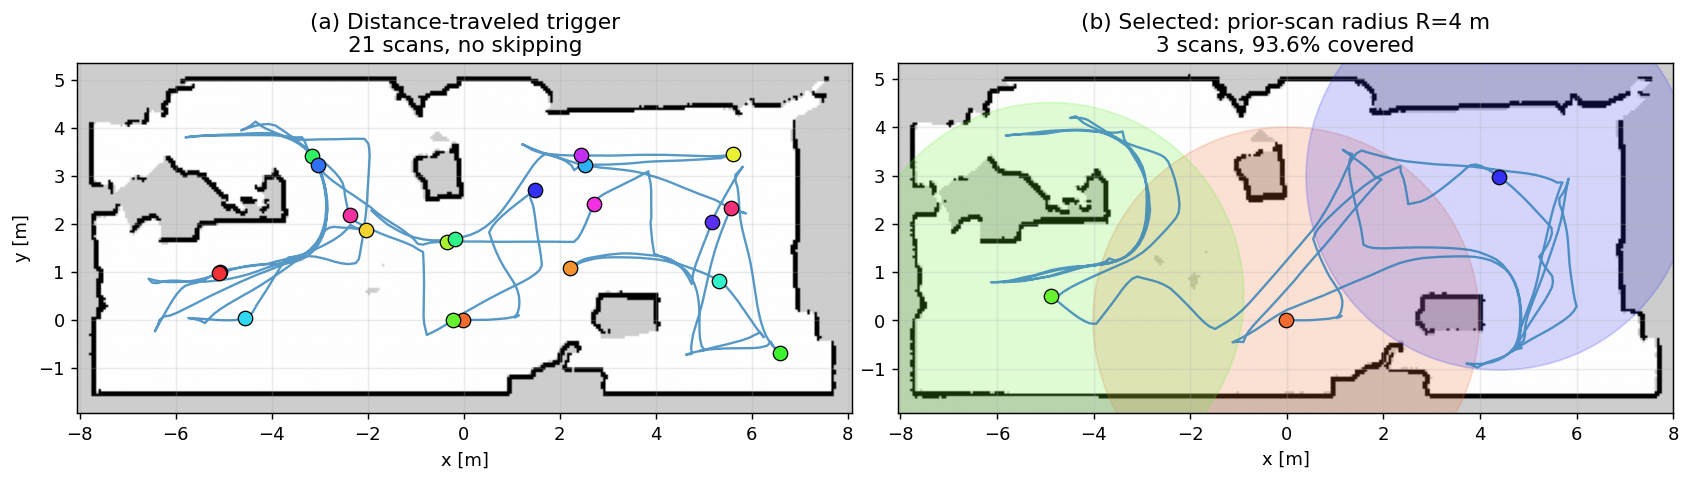
\includegraphics[width=\textwidth]{figures/fig6_strategy.png}
  \caption{Scan-triggering strategies overlaid on the Cartographer SLAM map
  (shaded disks: the skip radius $R$ around each scan; solid line: the robot
  trajectory; markers: scan positions). (a)~The distance-traveled trigger
  fires 21 scans. (b)~The prior-scan radius ($R=4$~m) maps the room with 3
  scans.}
  \label{fig:mapscan}
\end{figure}

\begin{figure}[!htb]
  \centering
  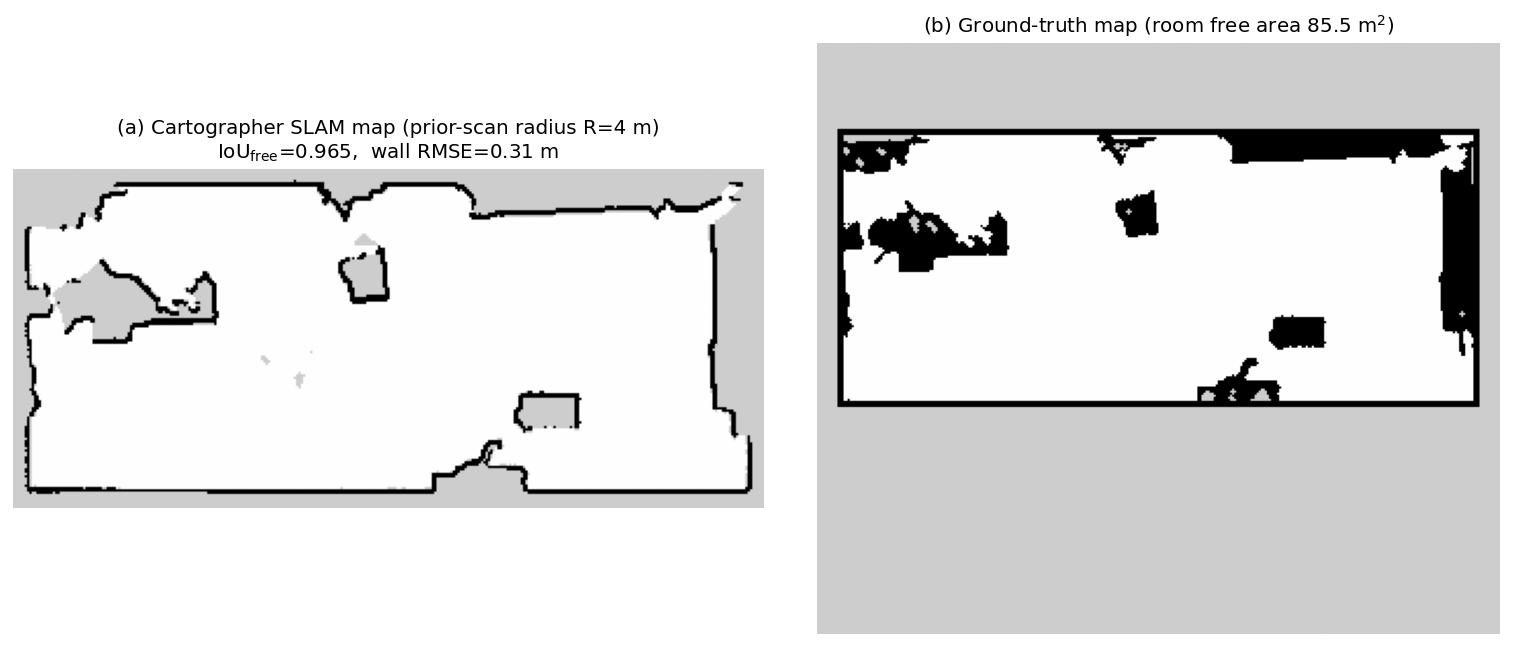
\includegraphics[width=0.92\textwidth]{figures/fig6_mapqual.png}
  \caption{Map quality of the selected run ($R=4$~m). (a)~The Cartographer
  occupancy map, $\mathrm{IoU}_{\mathrm{free}}=0.965$ and wall RMSE 0.31~m
  after translation alignment to ground truth. (b)~The ground-truth occupancy
  map of the test room.}
  \label{fig:mapqual}
\end{figure}

The proximity rule, however, judges coverage by Euclidean distance alone. The
remainder of this section evaluates the visibility-based policy of
Sections~\ref{sec:coverage} and~\ref{sec:placement} on two axes, LOS coverage
and stationary scan count. Four placement policies are compared throughout:
(i)~a \emph{uniform no-skip} reference that scans at every candidate---an
upper reference on the coverage attainable along a path; (ii)~the \emph{disk
spacing} baseline above; (iii)~the \emph{disk marginal-gain} baseline, which
applies the identical accept/skip rule as the proposed policy to the disk
coverage model; and (iv)~the proposed \emph{ray-cast visibility} policy.
Published TLS scan-planning methods are not applicable as online baselines
because they optimize viewpoints offline over a prior environment
model~\cite{tls-scanplanning,dehbi2021,knechtel2025}.

\subsection{Coverage Model and Single-Room Placement}
\label{subsec:exp-singleroom}

Figure~\ref{fig:concept} contrasted the two coverage models for a single scan
pose. On the full single-room world, the visibility stop-and-scan policy
places four scans and reaches 97.9\% LOS coverage
(Figure~\ref{fig:singleroom}). Varying the range bound $R\in\{5,6,10\}$~m
yields 97--98\% LOS in all cases (Figure~\ref{fig:rsweep}); larger $R$ needs
fewer scans but spreads them apart, reducing inter-scan overlap. $R=6$~m is
adopted for three reasons: it balances coverage against the scan-to-scan
overlap that registration benefits from; it keeps every cell claimed as
covered well inside the scanner's highest-accuracy band (3D point accuracy of
6~mm at 10~m~\cite{leica-blk360}); and it matches the local room scale, and
hence the occlusion scale, of the indoor environments targeted.

\begin{figure}[!htb]
\centering
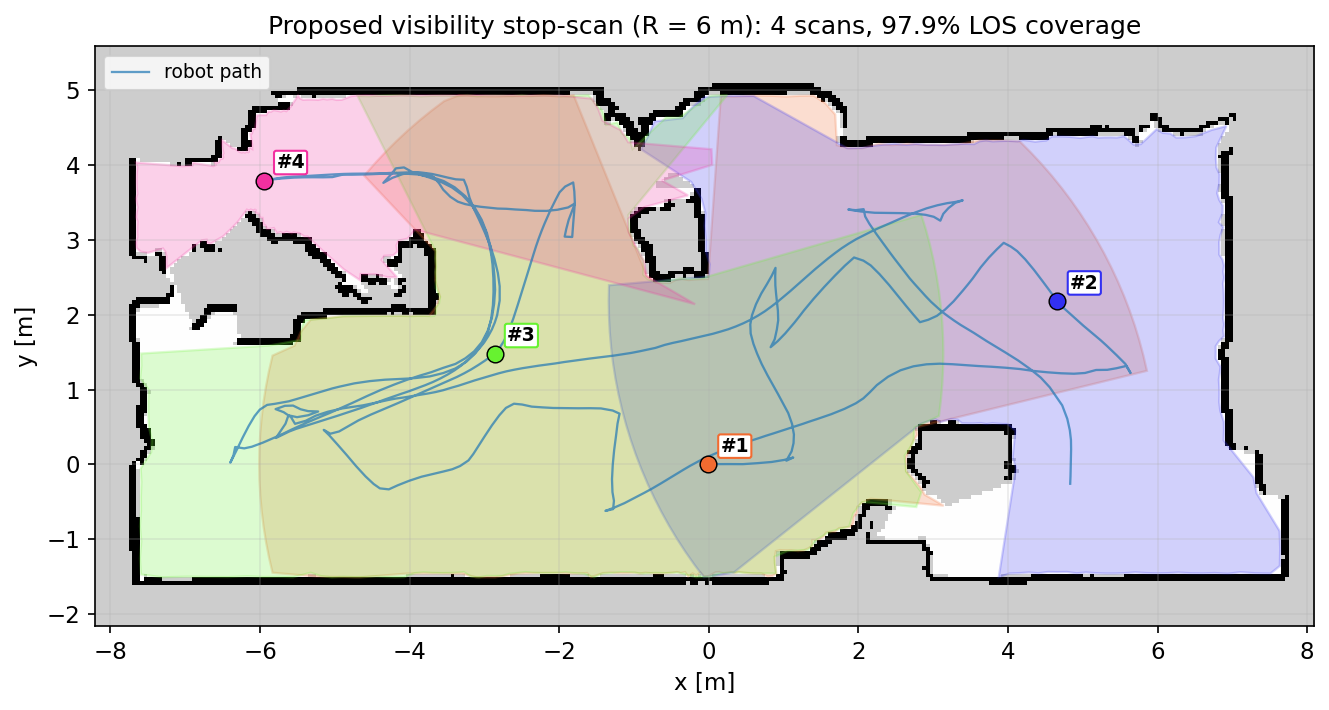
\includegraphics[width=0.7\linewidth]{figures/sen_fig2_singleroom_sota.png}
\caption{Visibility stop-and-scan on the single-room world ($R=6$~m): 4~scans,
97.9\% LOS coverage. Each accepted scan pose (marker) and its visibility
polygon share one color, indexed by scan order; the grayscale background is
the occupancy map and the blue line the robot path.}
\label{fig:singleroom}
\end{figure}

\begin{figure}[!htb]
\centering
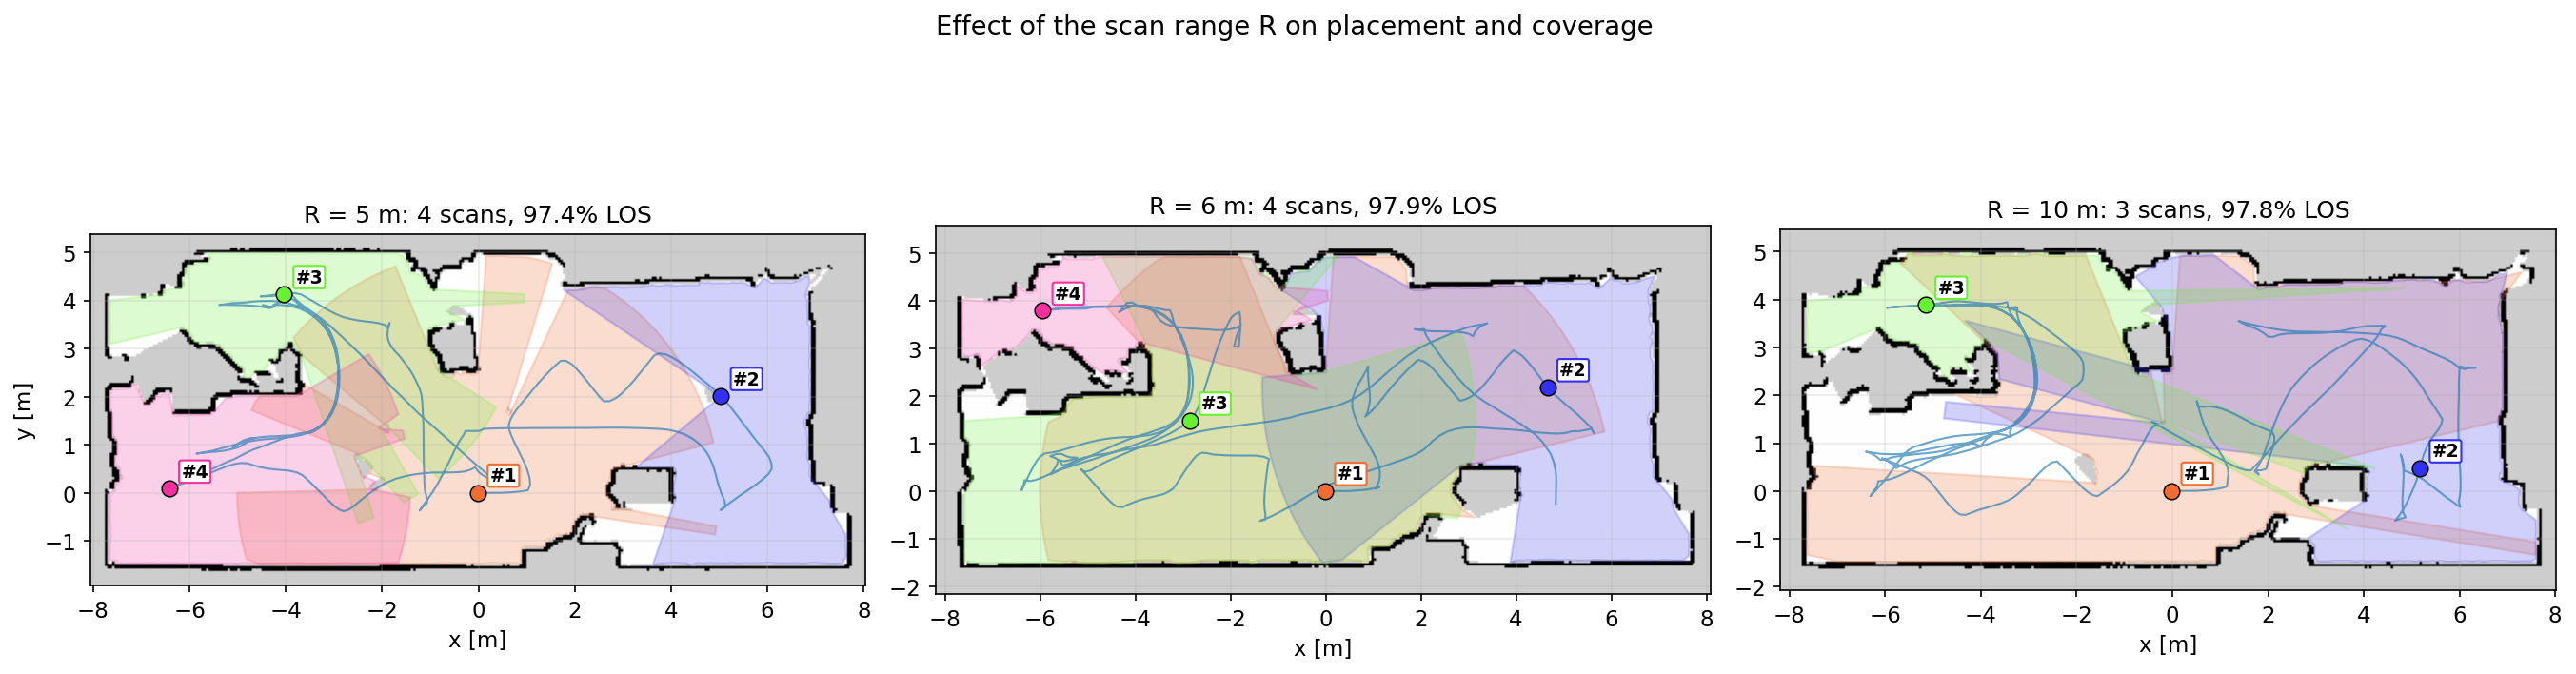
\includegraphics[width=0.95\linewidth]{figures/sen_fig3_R_sweep.png}
\caption{Effect of the range bound $R$ on placement and coverage for
$R=5/6/10$~m. Larger $R$ needs fewer scans but spreads them; $R=6$~m balances
coverage (97.9\%) against inter-scan overlap for registration.}
\label{fig:rsweep}
\end{figure}

\subsection{Controlled Skip-Rule Ablation}
\label{subsec:exp-ablation}

The decisive comparison isolates the only variable of interest, the
accept/skip decision, from the stochasticity of autonomous exploration. On a
fixed environment map and a fixed candidate sequence (a logged trajectory
resampled every 2~m of path length, denser than the live 3~m trigger so that no
policy is starved of decision opportunities), \emph{all} policies are
replayed, so they see identical maps and identical candidate poses and differ
only in which candidates they accept (Figure~\ref{fig:ablation}). This
deterministic, paired design removes the confound that, in live runs, which
rooms get mapped is dominated by navigation through narrow doorways rather
than by the skip rule.

Across $N=5$ single-room and $N=10$ multi-room trajectories, the visibility
rule raises LOS coverage from $77.0\pm4.9\%$ to $85.4\pm6.2\%$ in the
single-room world and from $77.0\pm6.4\%$ to $84.0\pm9.2\%$ in the three-room
world, at a cost of one to two additional scans on average
(Table~\ref{tab:ablation}, Figure~\ref{fig:summary}). The uniform no-skip
reference reaches $91.9\pm7.0\%$ and $86.6\pm9.9\%$ LOS, but at 28.0 and 40.8
scans on average; the visibility rule comes within 6.5 and 2.6 percentage
points of this brute-force upper reference while taking roughly an eighth as
many scans, and exceeds the disk baseline by $+8.4$ and $+7.0$ points. On
paths that traverse every room, where the disk rule's blindness to occlusion
is fully exercised, the per-path gain reaches $+21$ to $+23$ points. The disk
spacing rule is structurally capped: once two scans are placed, almost every
later candidate lies within $R$ of a prior scan, so it stops scanning even
though walls occlude much of the area it counts as covered.

The disk marginal-gain baseline isolates the coverage model from the
acceptance rule. Under the identical dual criterion, the disk model accepts
$2.6\pm0.5$ scans for $77.7\pm3.8\%$ LOS in the single-room world---essentially
the spacing rule's result---and $2.9\pm0.3$ scans for only $59.1\pm1.3\%$ LOS
in the multi-room world, markedly \emph{worse} than even the spacing rule.
Because $B_{\mathrm{disk}}$ claims area through partitions, the disk model's
own coverage bookkeeping saturates after the first few acceptances: every
later candidate appears almost fully covered, so the rule stops scanning while
whole rooms remain unobserved. That the same acceptance rule produces a
24.9-point LOS gap between the two coverage models in the multi-room world is
the sharpest form of this dissertation's claim: the deficiency lies in the
disk coverage model itself, not in the acceptance rule attached to it.

\begin{table}[htbp]
\centering
\caption{Controlled skip-rule ablation: four placement policies replayed on
the same fixed candidate sequences ($N=5$ single-room, $N=10$ multi-room
paths); mean\,$\pm$\,s.d. All policies traverse the identical path, so they
differ only in scan count. Source: \emph{Sensors}~\cite{kim2026sensors}.}
\label{tab:ablation}
\begin{tabular}{l l c c}
\toprule
\textbf{Environment} & \textbf{Coverage model} & \textbf{LOS coverage (\%)} & \textbf{Scans} \\
\midrule
\multirow{4}{*}{Single-room} & Uniform, no skip (reference) & $91.9\pm7.0$ & $28.0\pm13.0$ \\
                             & Disk, spacing rule (baseline) & $77.0\pm4.9$ & $2.0\pm0.0$ \\
                             & Disk, marginal-gain rule      & $77.7\pm3.8$ & $2.6\pm0.5$ \\
                             & Ray-cast visibility (ours)   & $\mathbf{85.4\pm6.2}$ & $3.6\pm0.9$ \\
\midrule
\multirow{4}{*}{Multi-room}  & Uniform, no skip (reference) & $86.6\pm9.9$ & $40.8\pm11.8$ \\
                             & Disk, spacing rule (baseline) & $77.0\pm6.4$ & $2.3\pm0.5$ \\
                             & Disk, marginal-gain rule      & $59.1\pm1.3$ & $2.9\pm0.3$ \\
                             & Ray-cast visibility (ours)   & $\mathbf{84.0\pm9.2}$ & $3.6\pm0.7$ \\
\bottomrule
\end{tabular}
\end{table}

\begin{figure}[!htb]
\centering
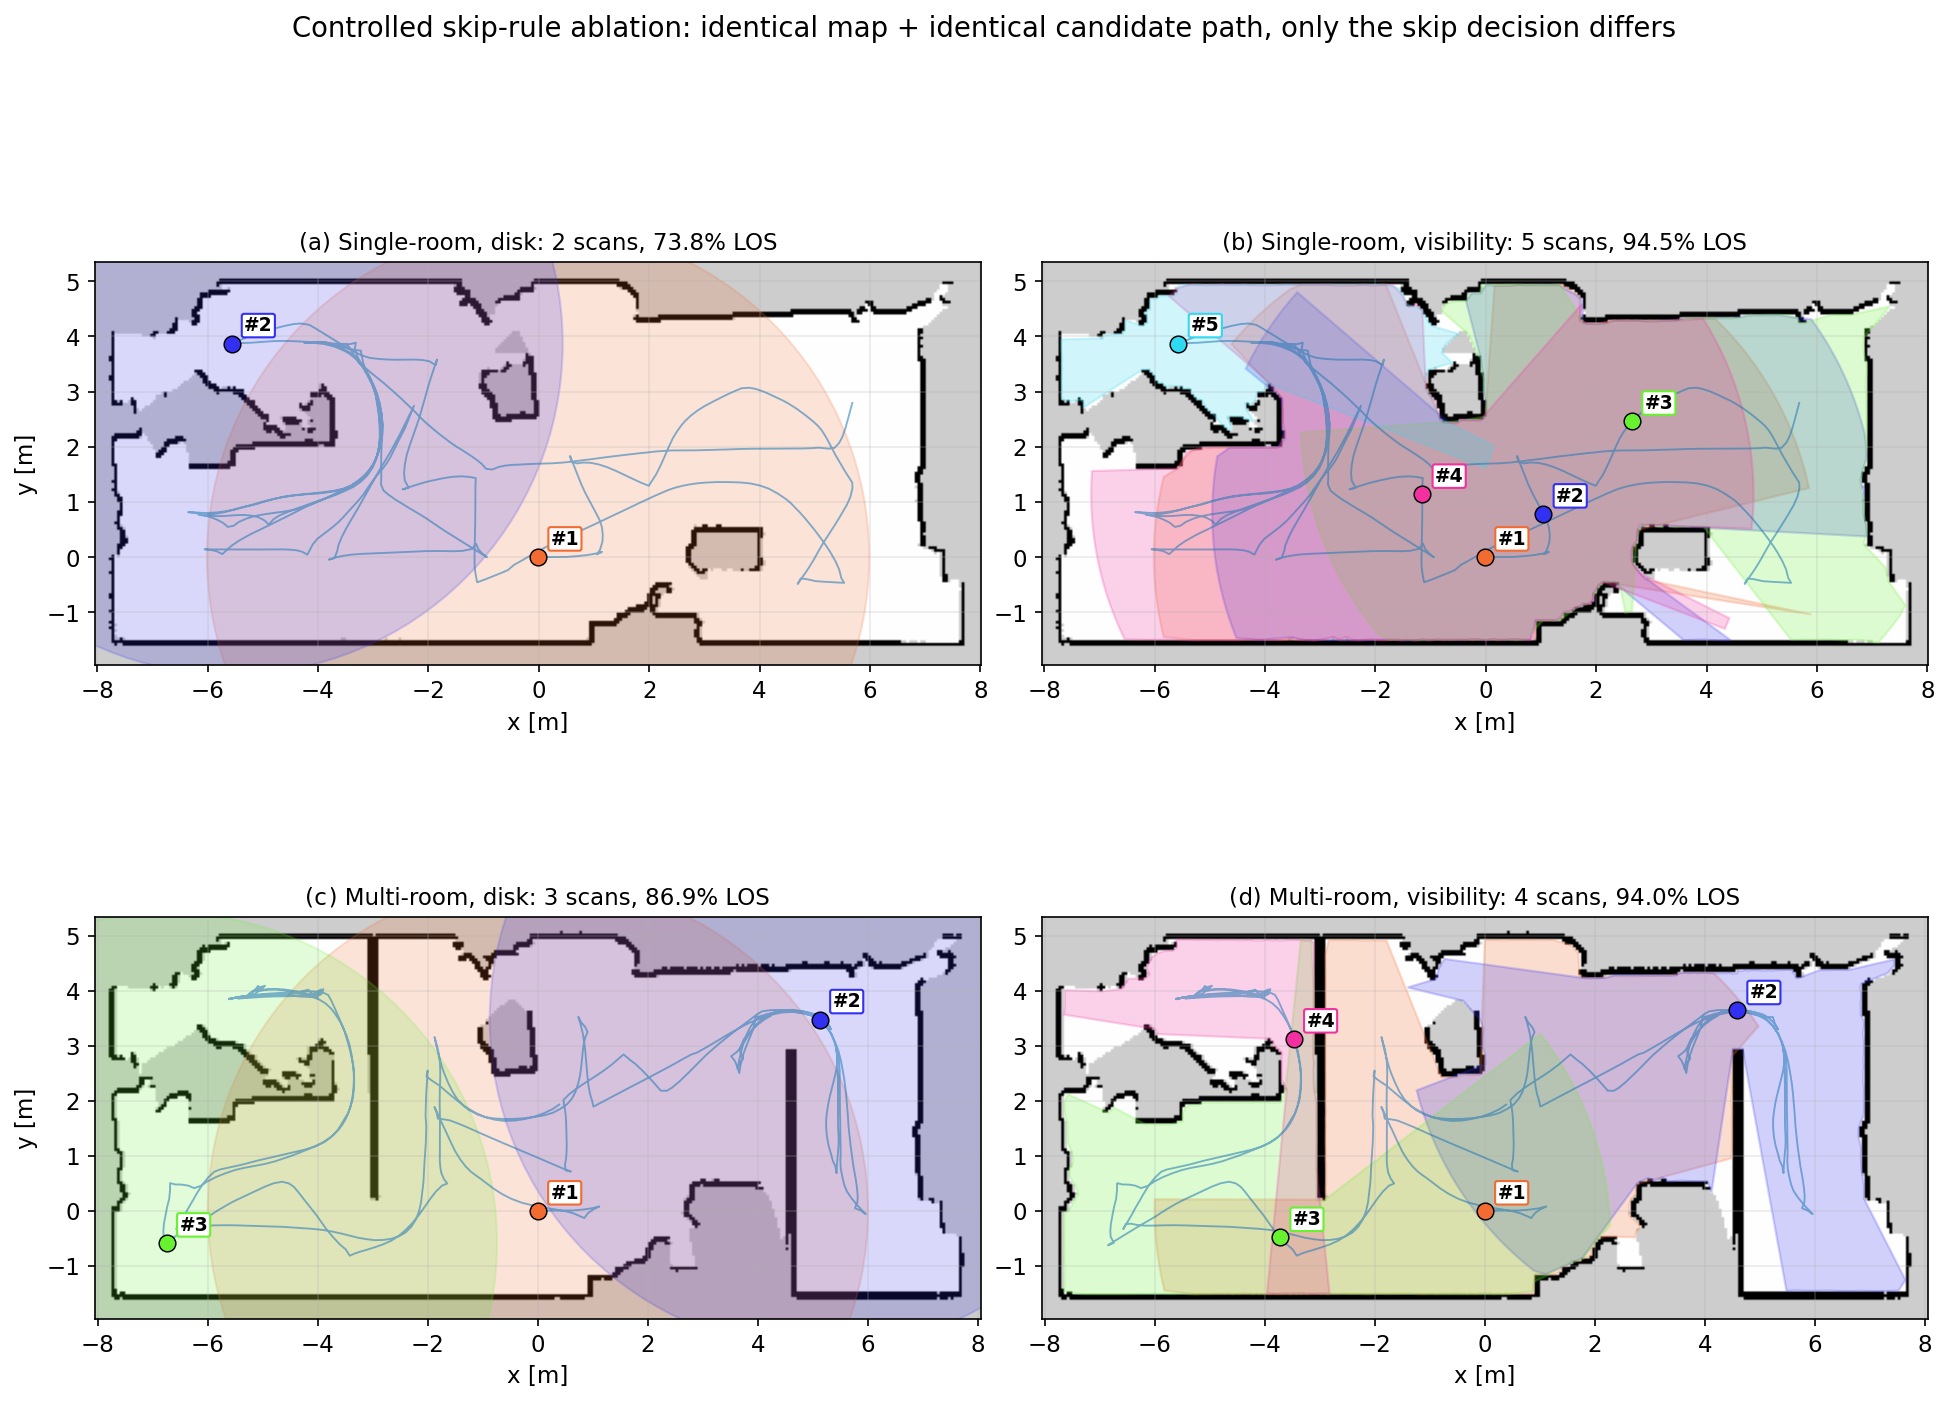
\includegraphics[width=0.95\linewidth]{figures/sen_fig5_skip_ablation.png}
\caption{Controlled skip-rule ablation on an identical map and candidate
path; only the skip decision differs. (a,b)~Single-room and (c,d)~multi-room,
under the disk spacing rule (a,c) and the visibility rule (b,d).}
\label{fig:ablation}
\end{figure}

\begin{figure}[!htb]
\centering
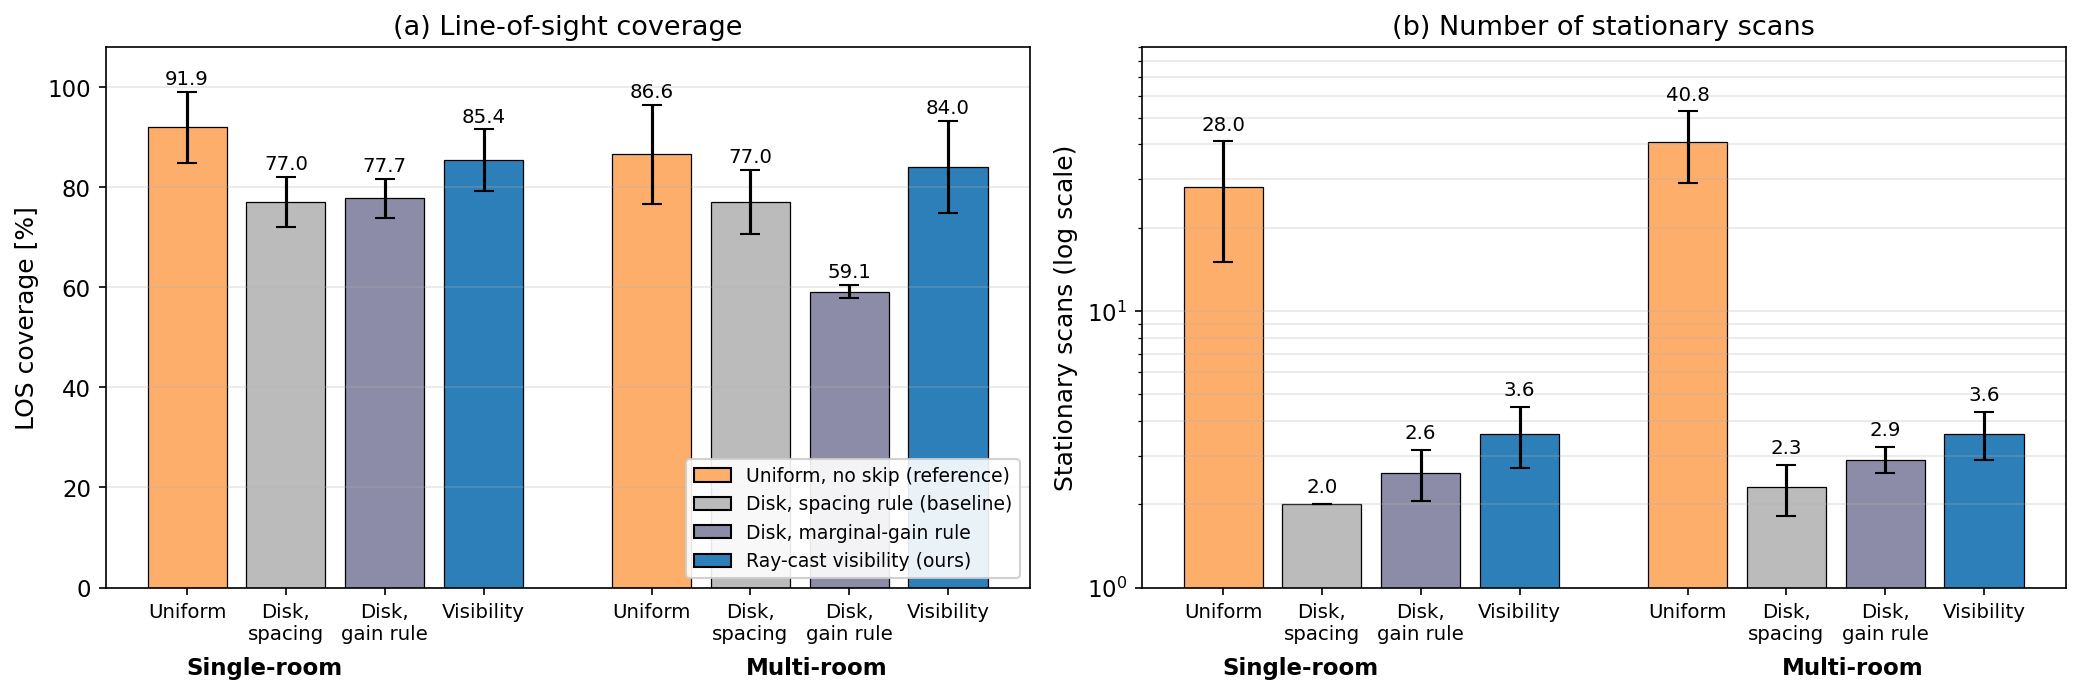
\includegraphics[width=0.95\linewidth]{figures/sen_fig7_summary.png}
\caption{Four-way skip-rule comparison on identical paths ($N=5$ single-room,
$N=10$ multi-room trajectories, paired per path). (a)~LOS coverage;
(b)~stationary scan count, log scale (mean\,$\pm$\,s.d.).}
\label{fig:summary}
\end{figure}

\subsection{Live Multi-Room Demonstration, Coverage Completion, and Parameter Sensitivity}
\label{subsec:exp-sensitivity}

Figure~\ref{fig:multiroom} shows a single live autonomous run on the
multi-room world under each coverage model. The disk policy stops after two
scans at 46.9\% LOS, having counted an entire room behind a partition as
covered through the wall; the visibility policy places one scan per room,
three in total, and reaches 95.1\% LOS. This run is presented as a qualitative
demonstration: in live runs on the partitioned world, which rooms get mapped
varies from run to run and dominates the measured coverage largely
independently of the skip rule, so the rigorous claim is the controlled
ablation above. With the coverage-completion phase enabled, the robot continues
after frontier convergence to drive into and scan the remaining uncovered
pockets: over $N=5$ runs this raises LOS coverage to $98.9\pm0.9\%$ using
$5.0\pm1.2$ total scans on average (3.2 frontier plus 1.8 completion scans),
with no unreachable pockets; a representative run reaches 99.6\% LOS
(Figure~\ref{fig:completion}).

\begin{figure}[!htb]
\centering
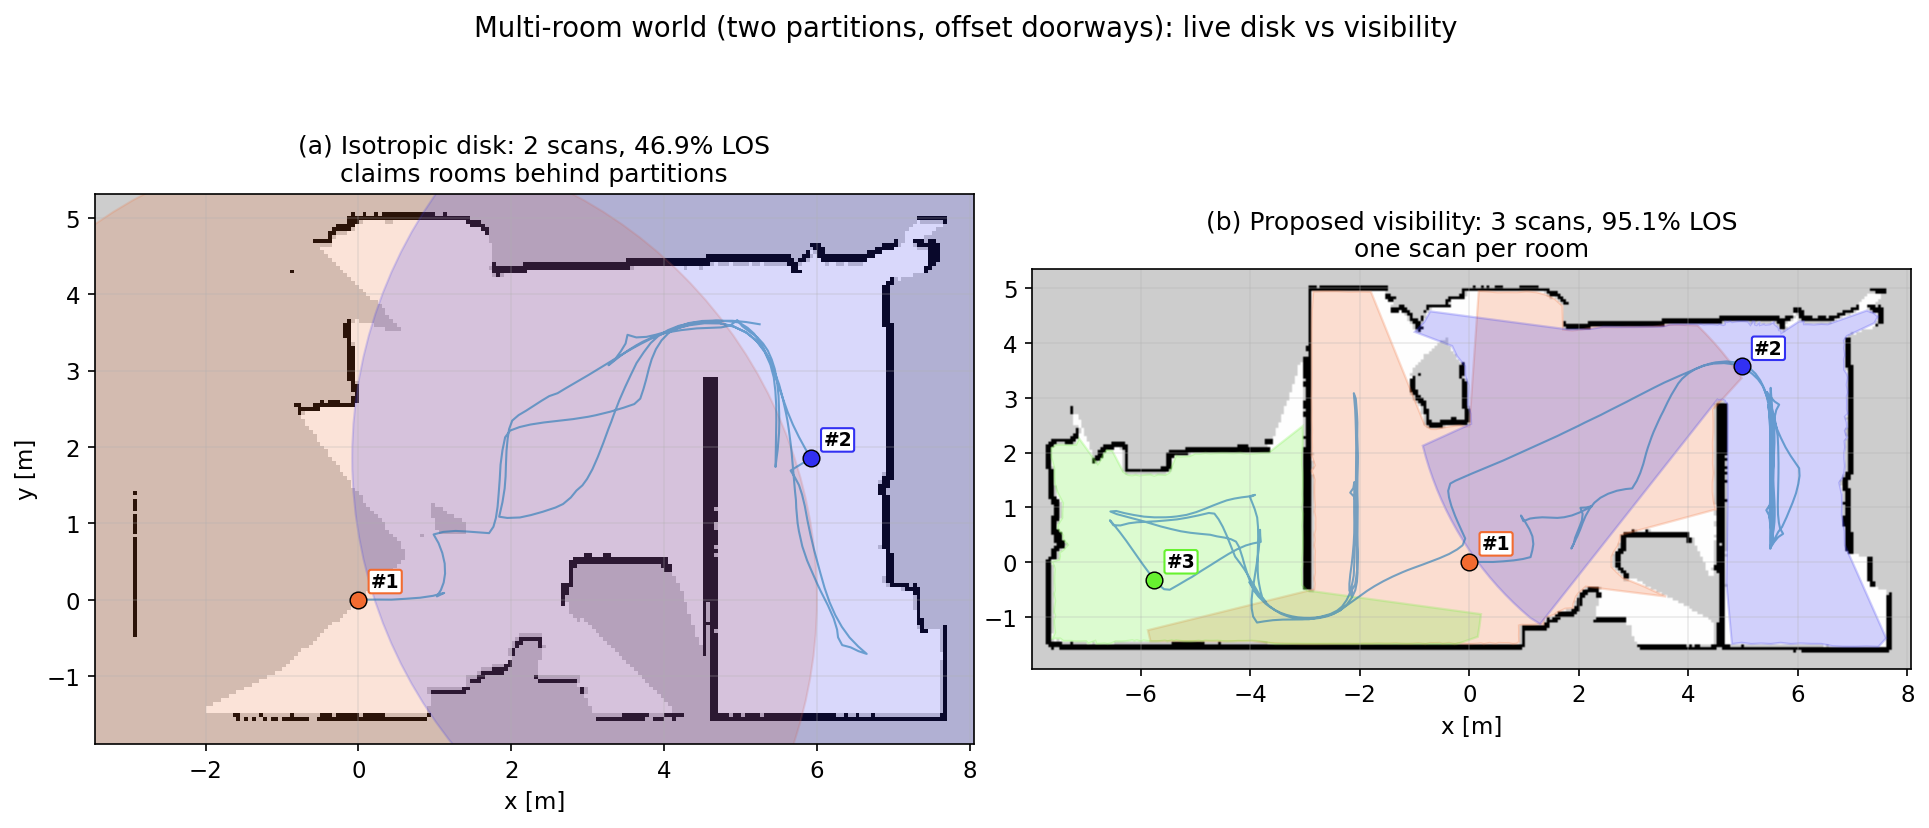
\includegraphics[width=0.95\linewidth]{figures/sen_fig4_multiroom_compare.png}
\caption{Multi-room world (two partitions, offset doorways): live disk vs.\
visibility. (a)~The disk model skips candidates within $R$ of a prior scan
through the partitions, giving 2~scans and 46.9\% LOS with a whole room
unscanned. (b)~The visibility model scans once per room, giving 3~scans and
95.1\% LOS.}
\label{fig:multiroom}
\end{figure}

\begin{figure}[!htb]
\centering
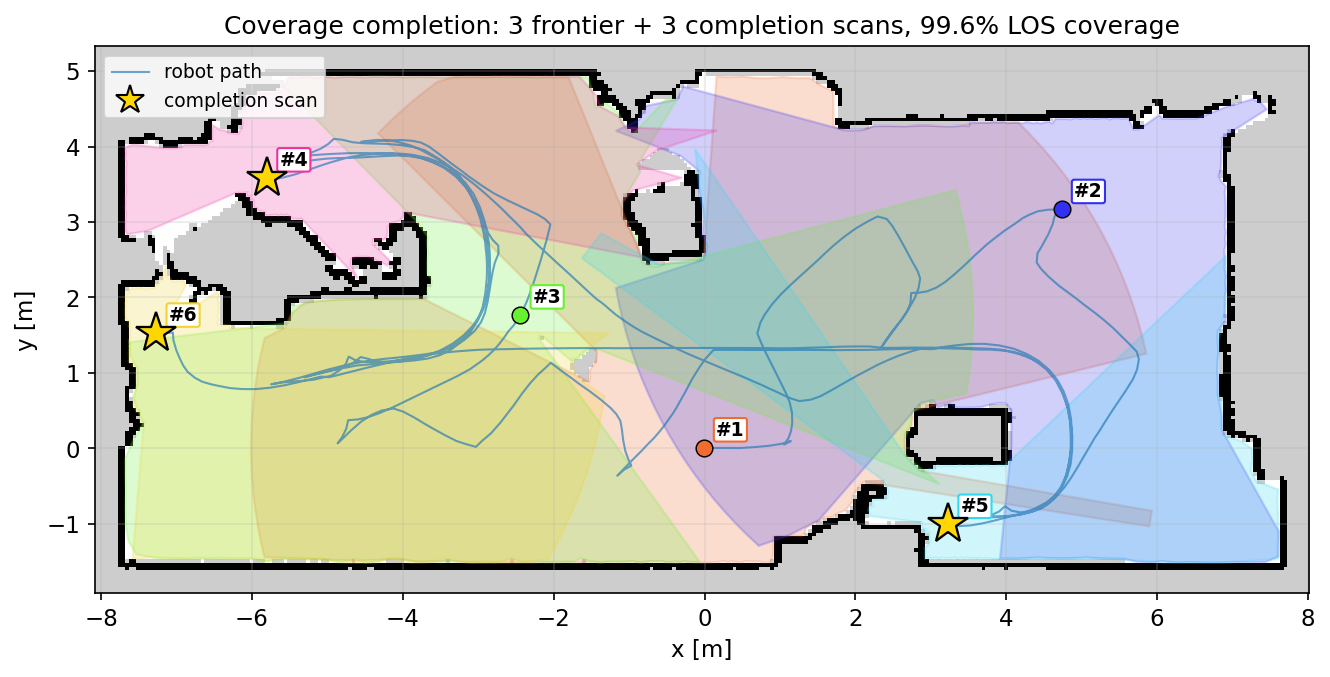
\includegraphics[width=0.7\linewidth]{figures/sen_fig6_completion.png}
\caption{Coverage completion. After frontier exploration, the robot drives
into each still-uncovered pocket and scans ($\star$) until none above the
minimum pocket area remains. Here 3~frontier $+$ 3~completion scans, 99.6\%
LOS.}
\label{fig:completion}
\end{figure}

The two skip thresholds are characterized by deterministic replay of the
visibility policy over the same fixed paths (Figure~\ref{fig:sweep}). Varying
the relative threshold $\tau$ over $[0.10,0.50]$ changes mean LOS coverage by
at most about two points (single-room $86.4\to84.3\%$; multi-room
$85.2\to84.0\%$) and mean scan count by less than one scan, so $\tau=0.30$ is
not a sensitive choice. The absolute threshold $A_{\min}$ is the operative
knob: $A_{\min}=5$~m$^2$ is the largest threshold whose mean LOS remains within
about five points of the most aggressive setting ($A_{\min}=1$~m$^2$) in both
environments (single-room 85.4 versus 90.7\%; multi-room 84.0 versus 85.7\%)
while already halving the scan count (3.6 versus 7.2 scans). Beyond the knee
the trade turns unfavorable: $A_{\min}=15$~m$^2$ saves only about one further
scan while coverage continues to erode ($85.4\to80.8\%$ and
$84.0\to83.1\%$). The operating point $\tau=0.30$, $A_{\min}=5$~m$^2$ was
fixed before the hardware campaign.

\begin{figure}[!htb]
\centering
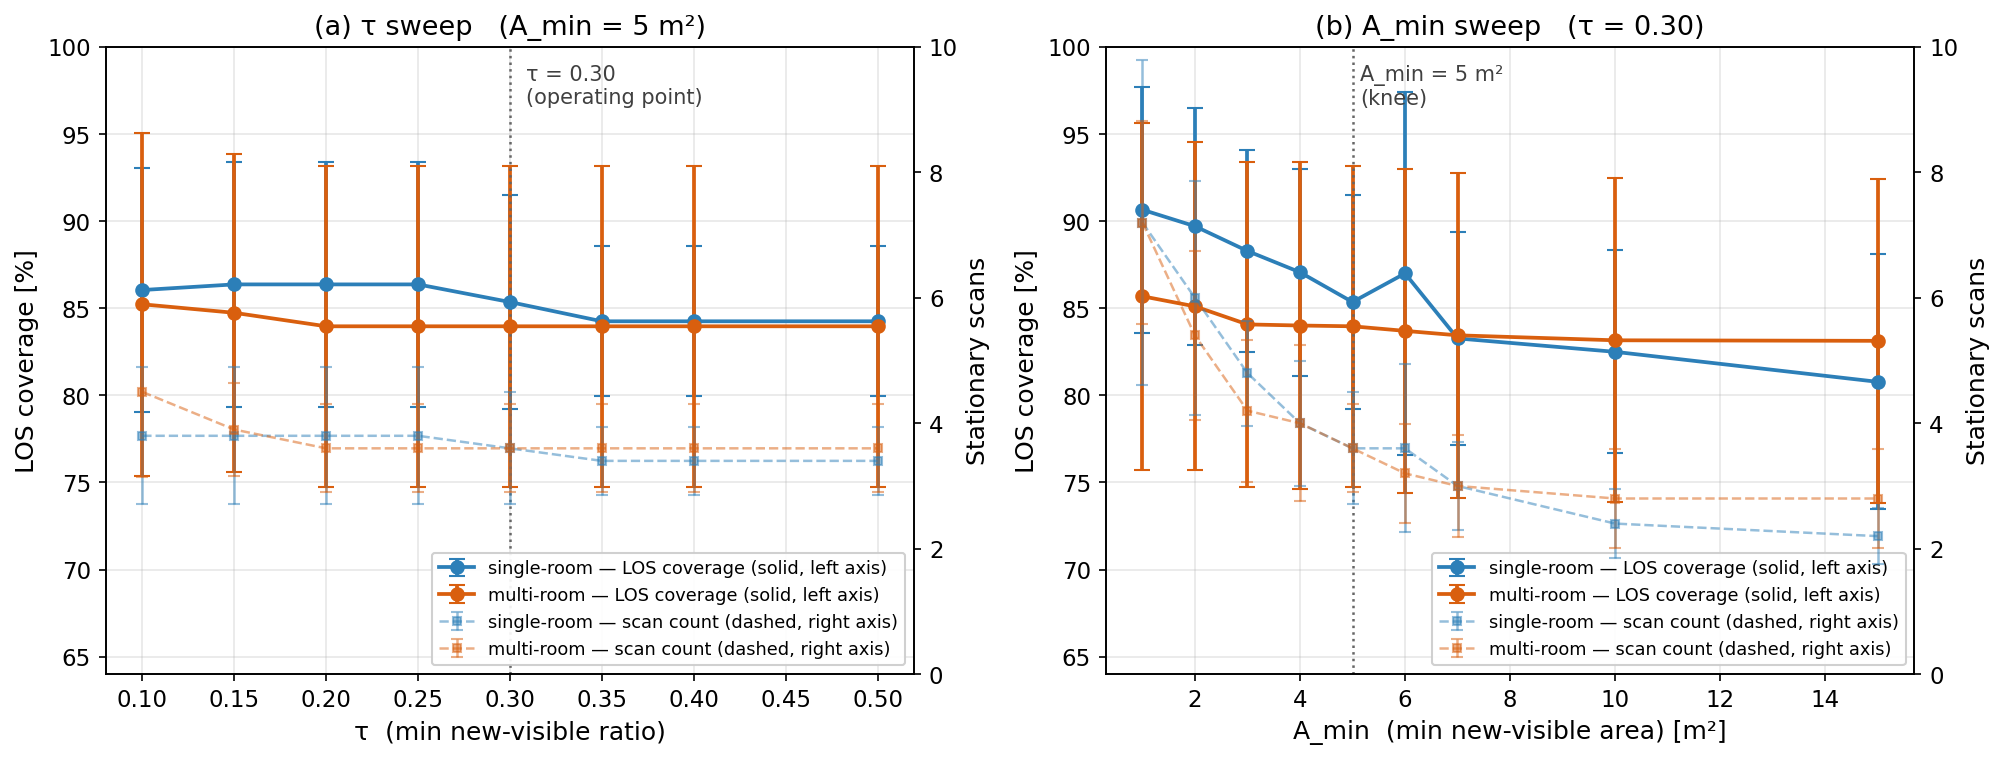
\includegraphics[width=0.95\linewidth]{figures/sen_fig8_param_sweep.png}
\caption{Parameter sweep by deterministic replay on the fixed candidate paths
(mean~$\pm$~s.d.). Solid curves: LOS coverage; dashed curves: scan count.
(a)~$\tau$ sweep at $A_{\min}=5$~m$^2$; (b)~$A_{\min}$ sweep at $\tau=0.30$,
knee marked.}
\label{fig:sweep}
\end{figure}

\subsection{Fully Autonomous On-Hardware Comparison}
\label{subsec:exp-hardware}

To test whether this behavior carries over to the physical platform, a fully
autonomous on-hardware comparison was conducted in the industrial test room:
RedBOT04 explores the room live under frontier exploration through the full
Nav2 stack while Cartographer builds the map online from the onboard 2D
LiDAR, and the stop-and-scan sequencer applies the placement policy in real
time; at each accepted pose the platform halts and the deck-mounted BLK360
acquires a full-dome stationary scan (Figure~\ref{fig:field}). Each run is
driven end to end by one skip rule---disk or visibility---so the comparison
exercises the entire pipeline on real hardware. Of the on-hardware runs, the
$N=4$ per policy that completed a room-spanning traverse are retained; two
additional early-terminated runs, in which frontier exploration stalled
shortly after start before the placement policy faced any consequential
decision, are discarded as failed trials independent of the skip rule. Every
run is evaluated on the single most complete SLAM map among the runs. Unlike
the simulated ablation, hardware runs cannot be paired, so this experiment
complements the confound-free ablation with ecological validity.

\begin{figure}[!htb]
\centering
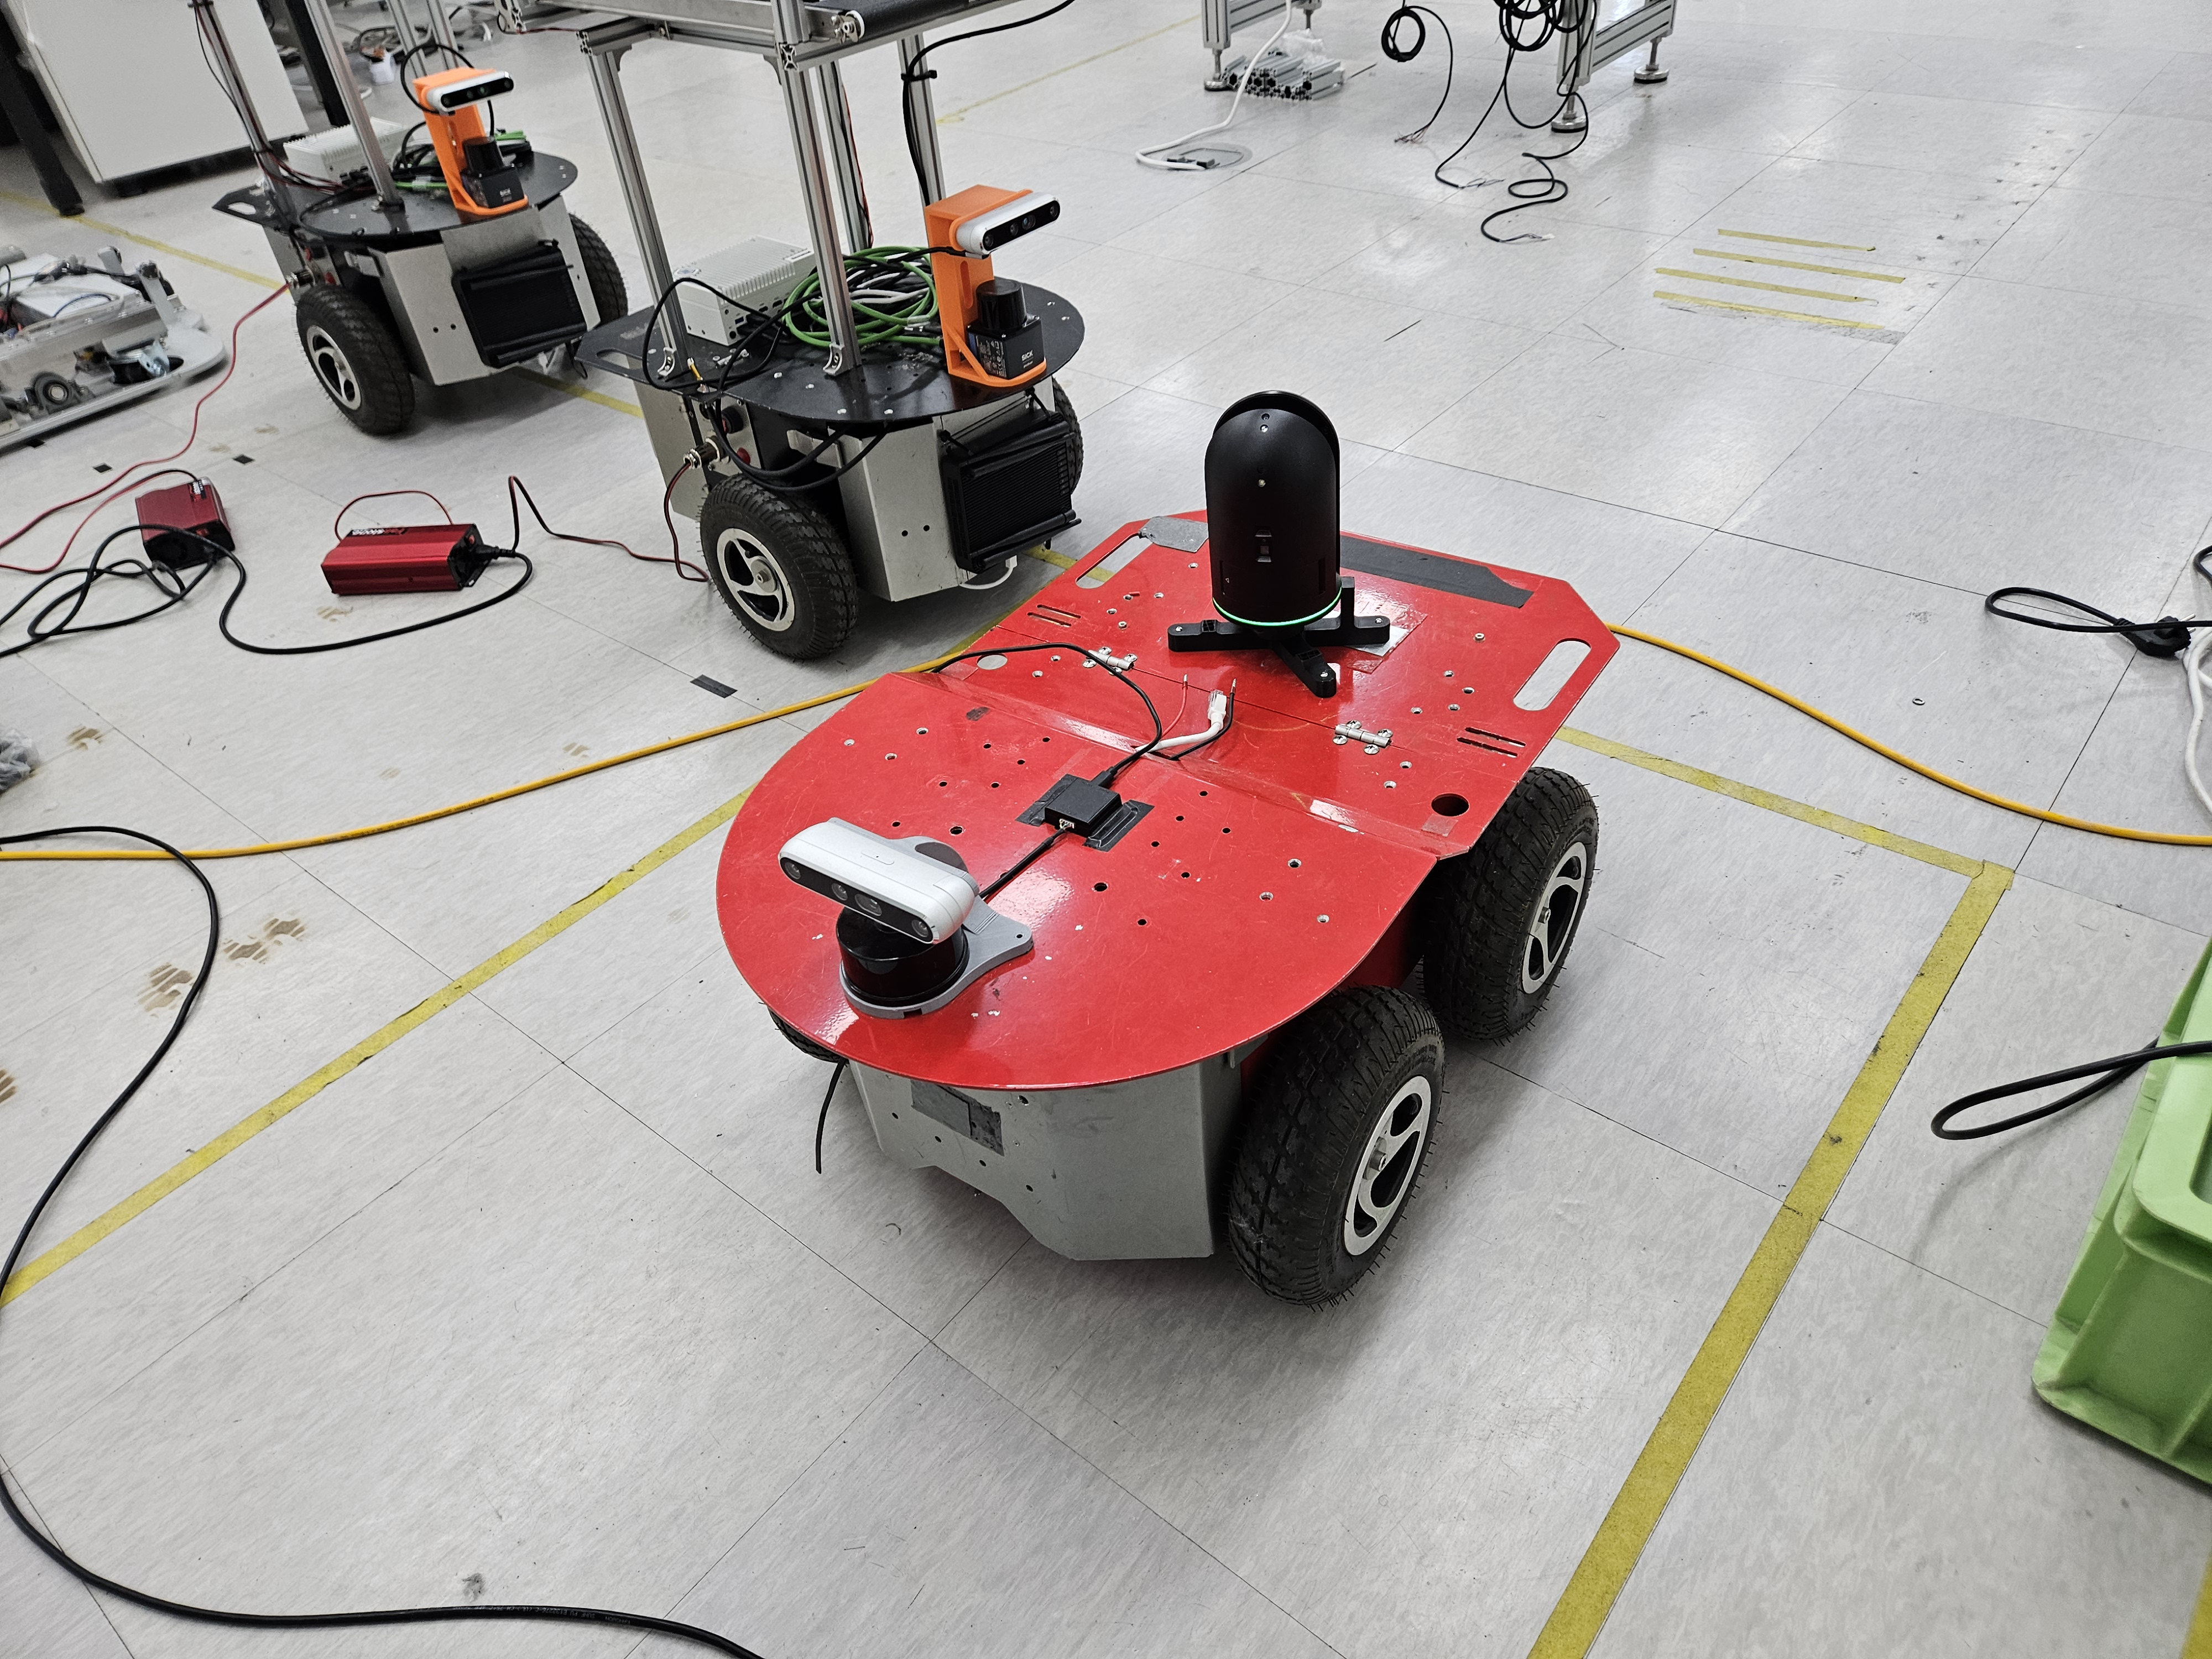
\includegraphics[width=0.82\linewidth]{figures/sen_fig13_redbot04_field.jpg}
\caption{RedBOT04 deployed in the industrial test room during the fully
autonomous on-hardware runs, with the Leica BLK360~G1 on its deck.}
\label{fig:field}
\end{figure}

The outcome reproduces the controlled ablation on the physical platform---a
platform kinematically and dimensionally different from the simulated
base---indicating that the effect is a property of the coverage model rather
than of any particular robot (Table~\ref{tab:fieldsim}, Figure~\ref{fig:fieldsim}).
The isotropic disk over-skips: it places only $1.8\pm0.5$ scans and, treating
floor behind the equipment island and furniture as covered, attains
$77.6\pm10.5\%$ LOS coverage with a large run-to-run variance, since whether
its few stations happen to see the occluded bays is largely incidental. The
visibility rule recognizes the occluded area as unseen, places $4.2\pm1.5$
scans, and covers $92.1\pm3.8\%$ of the free space reliably at the cost of
about two extra scans.

\begin{table}[htbp]
\centering
\caption{Fully autonomous on-hardware disk-versus-visibility comparison in the
physical test room ($N=4$ completed live runs per policy on RedBOT04; all
runs evaluated on the common reference map; mean~$\pm$~s.d.). Source:
\emph{Sensors}~\cite{kim2026sensors}.}
\label{tab:fieldsim}
\begin{tabular}{l c c}
\toprule
\textbf{Coverage model} & \textbf{Scans} & \textbf{LOS coverage (\%)} \\
\midrule
Isotropic disk (baseline)   & $1.8\pm0.5$ & $77.6\pm10.5$ \\
Ray-cast visibility (ours)  & $4.2\pm1.5$ & $\mathbf{92.1\pm3.8}$ \\
\bottomrule
\end{tabular}
\end{table}

\begin{figure}[!htb]
\centering
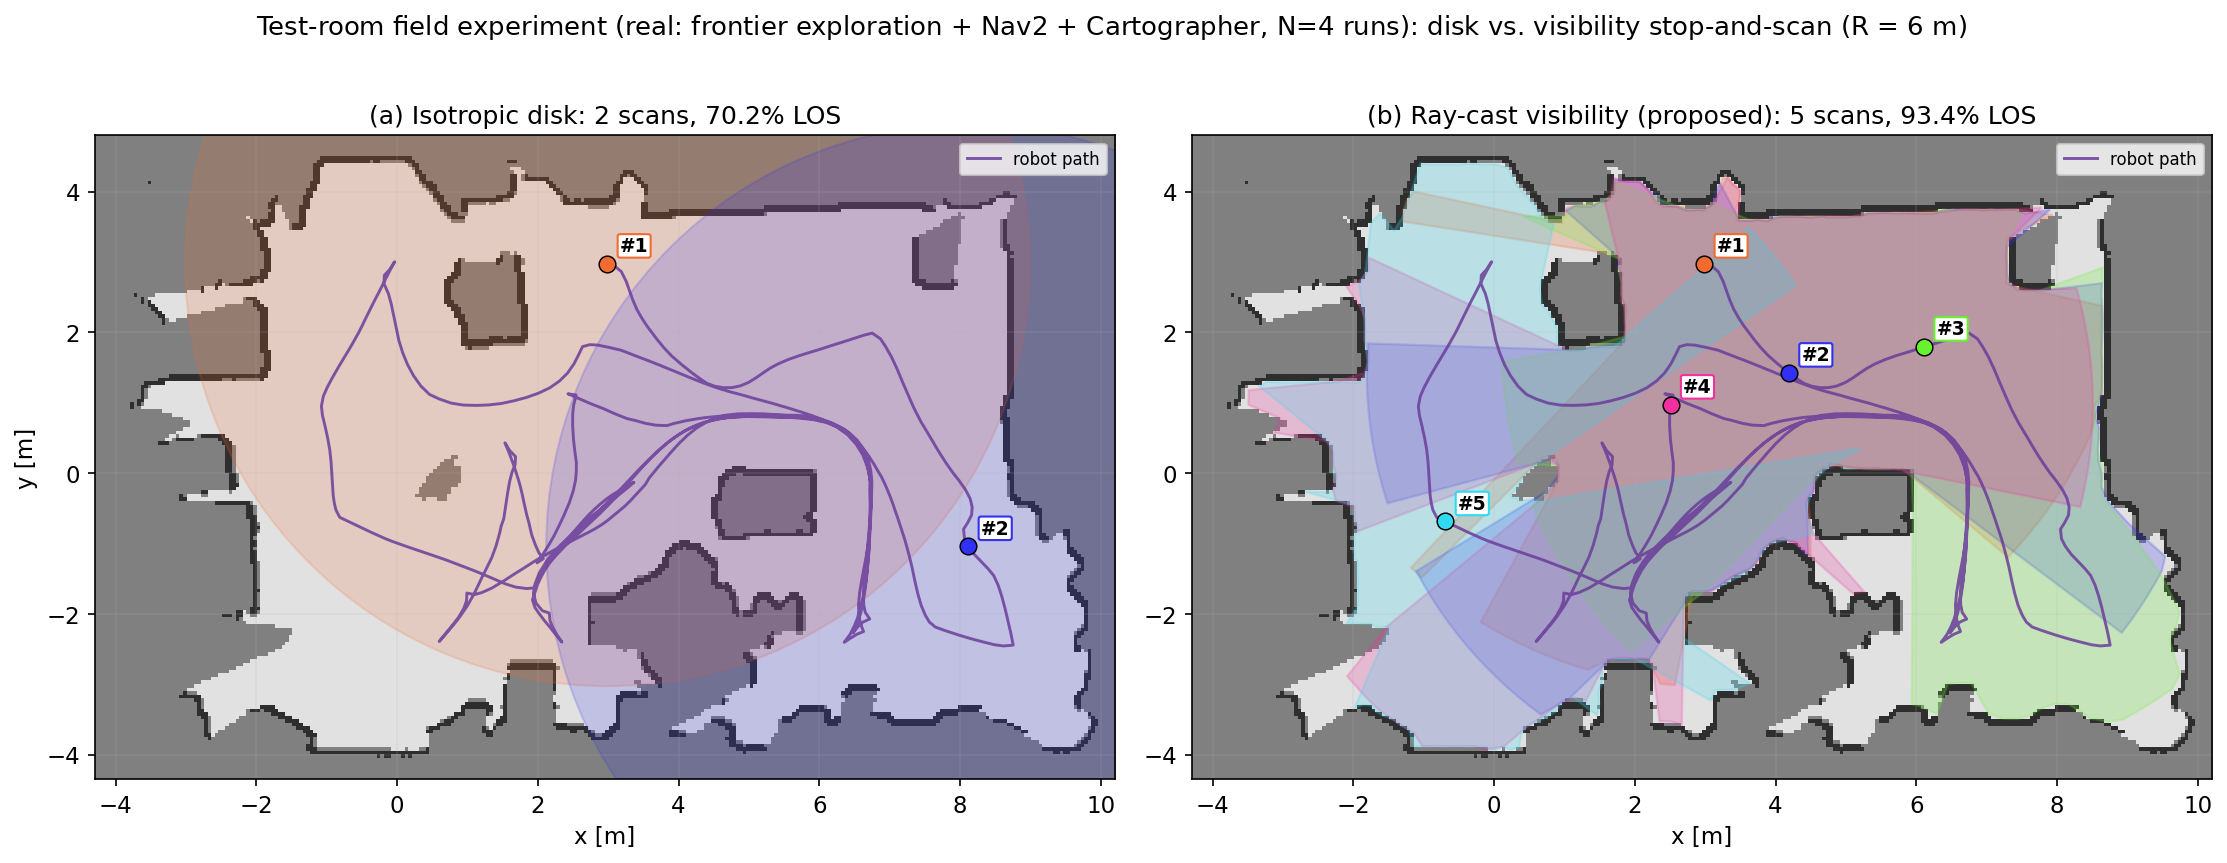
\includegraphics[width=\linewidth]{figures/sen_fig14_testroom_fieldsim.png}
\caption{Fully autonomous on-hardware comparison in the physical test room
(representative runs; $R=6$~m). Light gray: mapped free space; dark gray:
unmapped; black: occupied; purple line: autonomous robot path; colored
markers: placed scans with their coverage regions. (a)~Disk spacing rule;
(b)~visibility rule.}
\label{fig:fieldsim}
\end{figure}

\subsection{Survey-Grade Registration of the Autonomously Acquired Scans}
\label{subsec:exp-registration}

The remaining question is whether the scans each rule produces meet the
survey-grade premise. The BLK360 scans of every completed run were registered
offline, each run as an independent project under identical settings, in Leica
Cyclone REGISTER~360 PLUS using cloud-to-cloud alignment without artificial
targets (Table~\ref{tab:registration}). All four visibility runs registered at
survey grade: their networks comprise 3--6 setups joined by 3--13 pairwise
links, the bundle adjustments converged at 4--5~mm with overall overlaps of
84--88\%, and every individual link fell within the software's highest quality
band (per-link overlaps 74--92\%, errors 3--6~mm). The 4--5~mm bundle
residuals are of the same order as the scanner's stated single-setup accuracy.
The registered clouds reconstruct the room as a single coherent model
(Figures~\ref{fig:realreg} and~\ref{fig:regcloud}). The disk runs tell a
structurally different story: the three disk runs that placed two scans each
registered as a two-setup network with a single link (75--85\% overlap,
2~mm), and the fourth disk run placed only one scan and therefore admits no
registration at all. The low single-link residuals should not be read as
superior registration: with one link there is no redundancy, so the alignment
is not cross-checked by any independent constraint, and the resulting model
covers correspondingly less of the room. Bundle strengths are moderate
(38--48\%) across runs, reflecting the corridor-like traverses the explorer
takes; a loop-closing station layout, which the coverage-completion phase
naturally drives, would raise this redundancy measure.

\begin{table}[htbp]
\centering
\caption{Per-run offline registration of the autonomously acquired scans
(Leica Cyclone REGISTER~360 PLUS; cloud-to-cloud, no targets, identical
settings). Every link of every registered network lies within the software's
highest quality band (maximum error $\le15$~mm). Source:
\emph{Sensors}~\cite{kim2026sensors}.}
\label{tab:registration}
\begin{tabular}{l l c c c c}
\toprule
\textbf{Policy} & \textbf{Run} & \textbf{Setups} & \textbf{Links} & \textbf{Overall overlap (\%)} & \textbf{Bundle error (mm)} \\
\midrule
Visibility & 1 & 3 & 3  & 86 & 5 \\
Visibility & 2 & 6 & 13 & 86 & 5 \\
Visibility & 3 & 5 & 10 & 84 & 5 \\
Visibility & 4 & 3 & 3  & 88 & 4 \\
\midrule
Disk & 1 & 1 & 0 & \multicolumn{2}{c}{not registrable (single setup)} \\
Disk & 2 & 2 & 1 & 75 & 2 \\
Disk & 3 & 2 & 1 & 85 & 2 \\
Disk & 4 & 2 & 1 & 84 & 2 \\
\bottomrule
\end{tabular}
\end{table}

\begin{figure}[!htb]
\centering
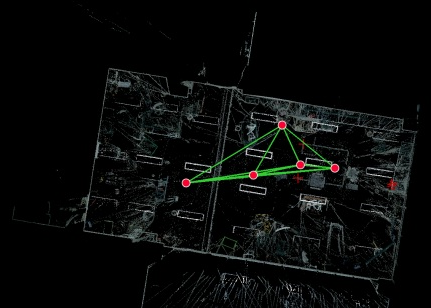
\includegraphics[height=5.0cm]{figures/sen_fig15_reg_network_vis.png}\hfill
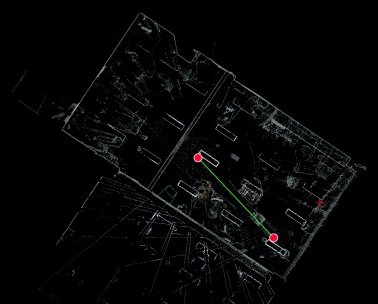
\includegraphics[height=5.0cm]{figures/sen_fig16_reg_network_disk.png}
\caption{Registered scan-station networks (top-down view; red markers are
setup positions, green edges are cloud-to-cloud links). (Left)~Visibility
run~3: five setups joined by ten redundant links reconstruct the room as a
single coherent model. (Right)~Disk run~4: two setups joined by a single
link---a minimal network with no redundant constraint.}
\label{fig:realreg}
\end{figure}

\begin{figure}[!htb]
\centering
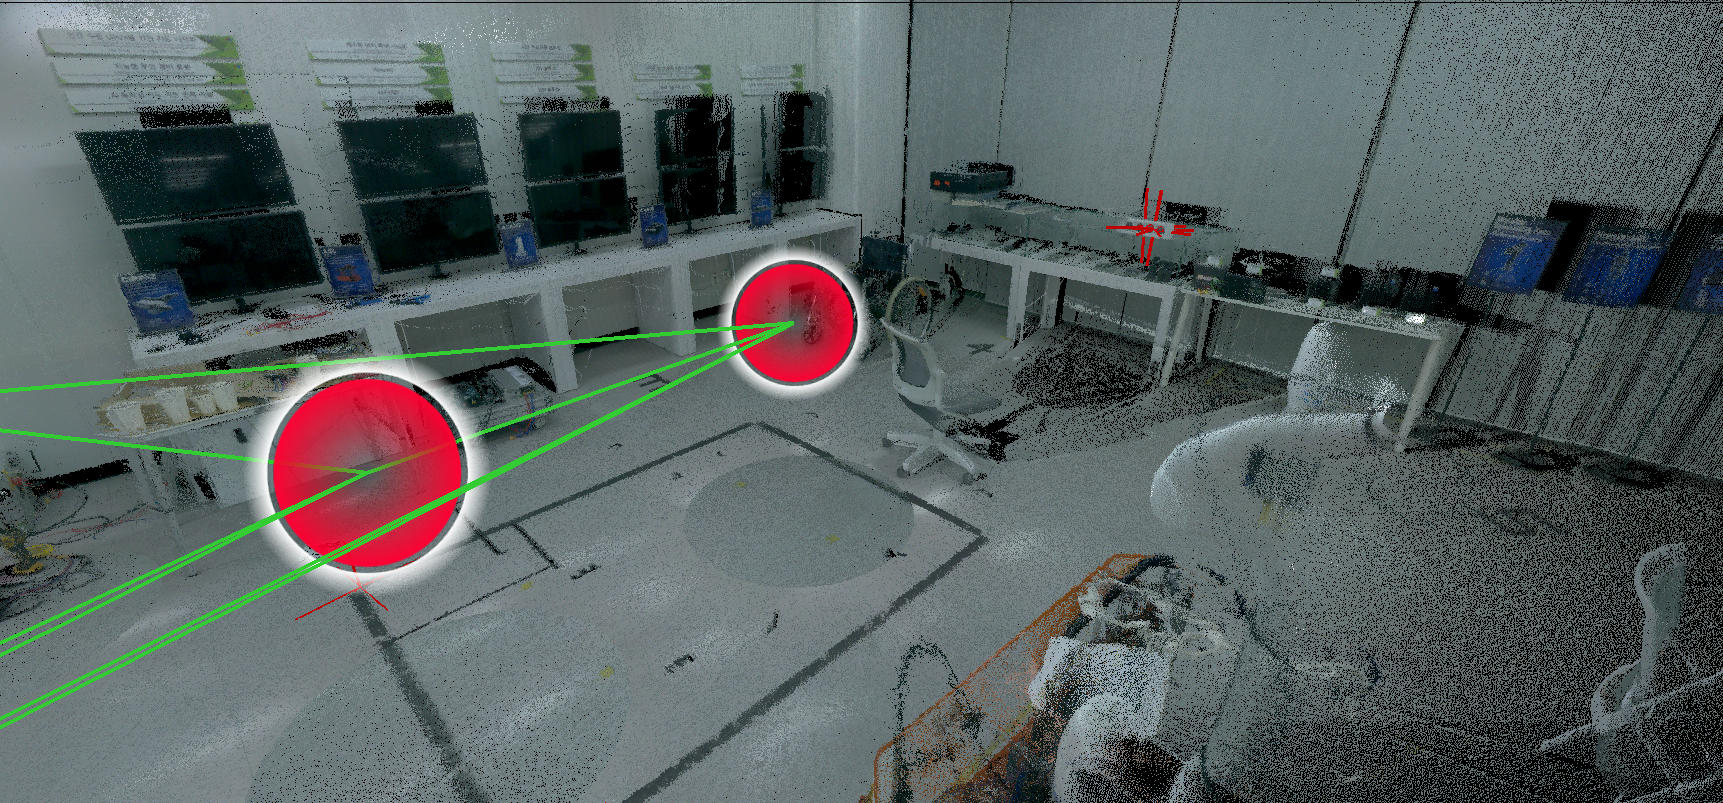
\includegraphics[width=0.49\linewidth]{figures/sen_fig17_regcloud_wall.png}\hfill
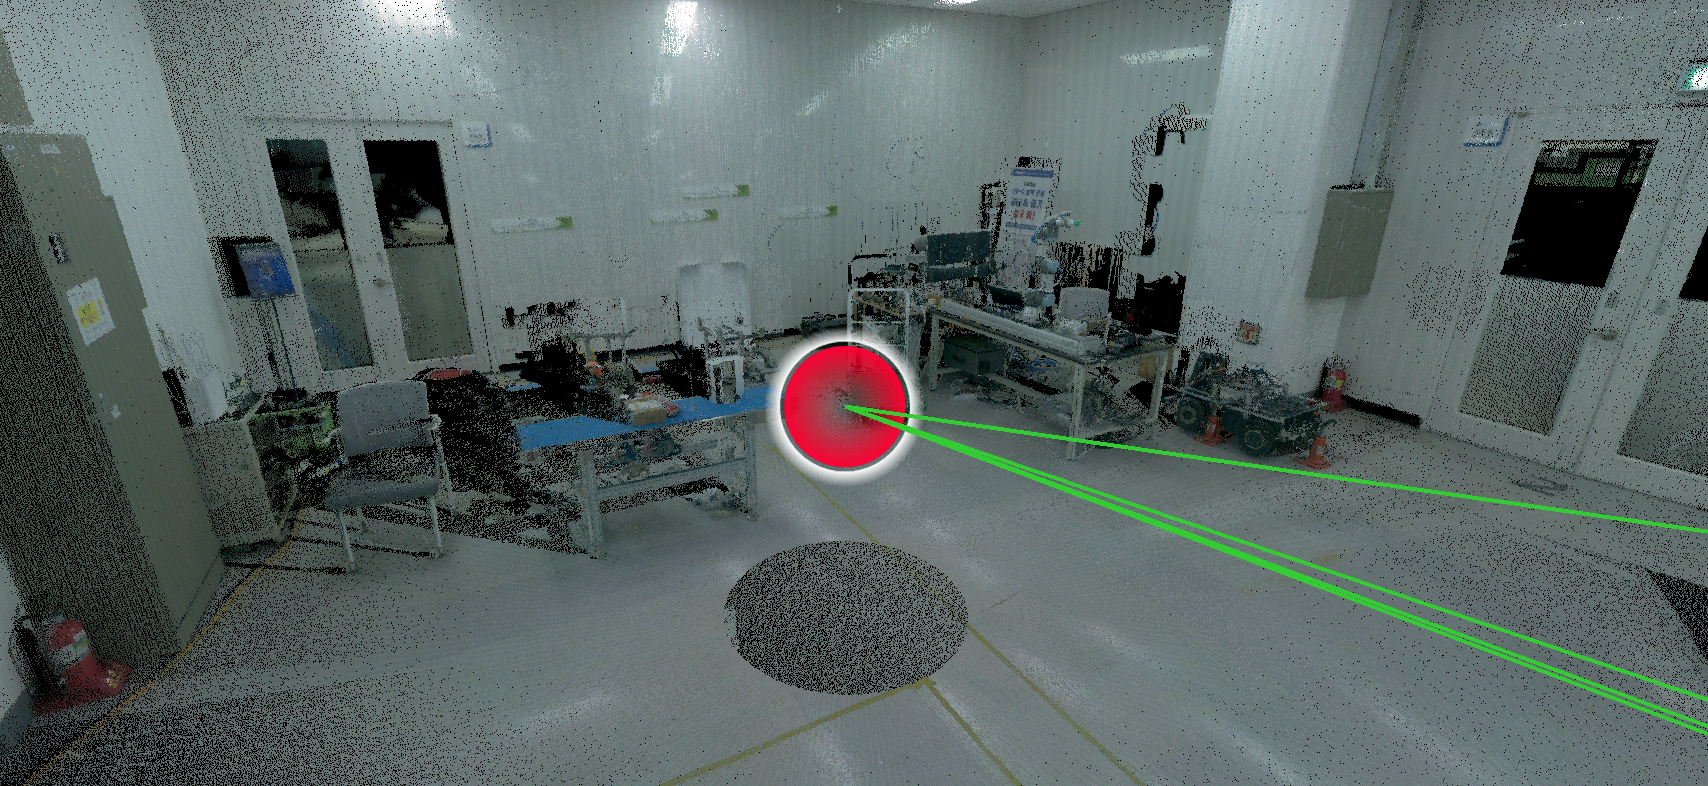
\includegraphics[width=0.49\linewidth]{figures/sen_fig18_regcloud_equipment.png}
\caption{Interior views of the registered colorized point cloud of visibility
run~3 along two diagonal directions: toward the display wall (left) and toward
the equipment side (right).}
\label{fig:regcloud}
\end{figure}

Together, the live comparison establishes that the visibility rule, not the
disk rule, reliably produces high-LOS scan placements, and the per-run
registration establishes that those placements consistently yield
survey-grade, bundle-verifiable scan networks, while disk placements do not
even guarantee a registrable network. The registered T2 and T3 clouds of
Table~\ref{tab:scenes} are the products of this subsystem that enter the
semantic modeling experiments below.

\section{Segmentation: Repeatability, Filtering, and Backbone Selection}
\label{sec:exp-seg}

\subsection{Backbone Selection against Learned Alternatives}
\label{subsec:exp-backbone}

The DBSCAN\,+\,Uni3D backbone was chosen against learned alternatives on a
wall-removed industrial scene of the test room (122.7~K points after
structural-plane removal; Figure~\ref{fig:nowallscene}). Because no point-level
ground truth exists for this scene, the metrics are deliberate screening
proxies: point \emph{coverage}, the fraction of input points assigned to some
object; the fraction of objects the open-vocabulary classifier cannot name
(\emph{unnameable}, a boundary-quality proxy because poor cuts produce more
unrecognizable fragments); and label diversity (Table~\ref{tab:backbones}).
For segmentation, the geometric clustering is compared against two
ScanNet-pretrained deep models, the superpoint-transformer instance segmenter
SPFormer~\cite{sun2023spformer} and the semantic-segmentation backbone Point
Transformer~V3~\cite{wu2024ptv3}, with every object subsequently named by the
same Uni3D classifier; for classification, Uni3D is compared against the
depth-projection classifier PointCLIP~V2~\cite{zhu2023pointclipv2}. Two further
instance segmenters, Mask3D~\cite{schult2023mask3d} and
Part2Object~\cite{shi2024part2object}, could not be evaluated because both
depend on a sparse-convolution backend incompatible with the experimental GPU.

\begin{figure}[!htb]
  \centering
  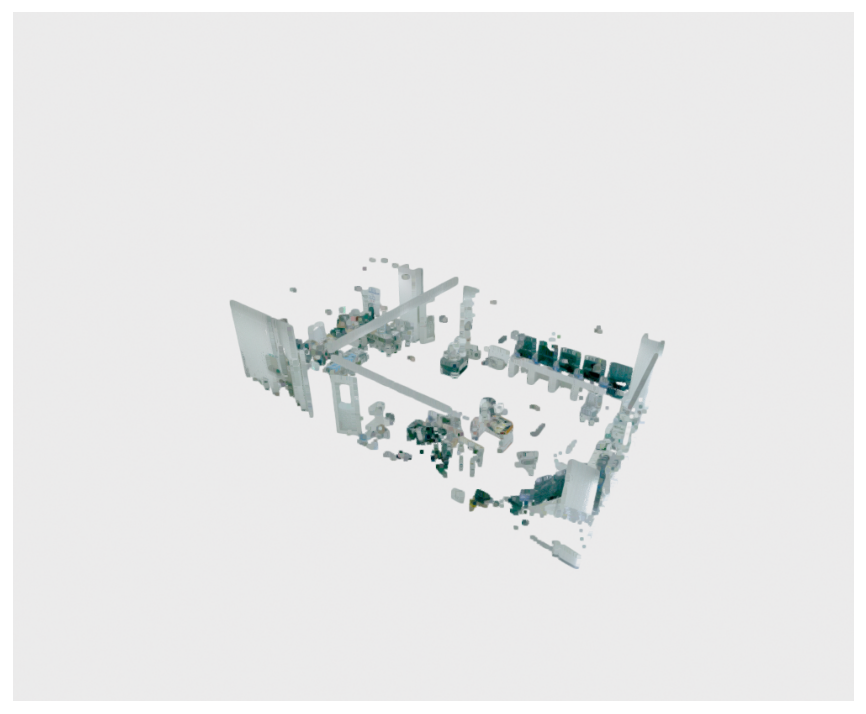
\includegraphics[width=0.7\textwidth]{figures/fig6_nowall.png}
  \caption{The backbone-selection scene: the test-room scan after
  structural-plane removal, shown in raw RGB (122{,}738 points). Only the
  object clutter remains, each connected cluster forming a candidate object.}
  \label{fig:nowallscene}
\end{figure}

\begin{table}[htbp]
\centering
\caption{Segmentation$\times$classification backbone comparison on the
wall-removed industrial scene (screening proxies; no point-level ground
truth). The PTv3 row is a semantic-segmentation head whose outputs are not
instance-comparable and is included only to document why closed-set semantic
heads were screened out.}
\label{tab:backbones}
\begin{tabularx}{\textwidth}{l c c c X}
\toprule
\textbf{Pipeline} & \textbf{Coverage} & \textbf{Unnameable} & \textbf{Classes} & \textbf{Dominant failure} \\
\midrule
\textbf{DBSCAN + Uni3D} & \textbf{98.3\%} & \textbf{23.3\%} & 13 & unlabeled coverage \\
SPFormer + Uni3D & 51.1\% & 45.9\% & 9 & furniture bias (chair 67/88) \\
PTv3 (semantic) & --- & --- & 17/20 emitted & 46\% ``wall'' after wall removal \\
DBSCAN + PointCLIP~V2 & 98.3\% & --- & 1--7 & collapse (pipe 23/30) \\
\bottomrule
\end{tabularx}
\end{table}

On every proxy, the geometric segmenter outperforms the deep closed-set model
on this out-of-distribution scene (Figure~\ref{fig:segcompare}). SPFormer
assigns only about half of the points to objects, because it fires only on
regions resembling its indoor-furniture training classes and lets genuine
industrial and robotic structure fall through; it over-segments the scene into
many partial or cross-object fragments that the classifier can no longer name,
and its label space is closed to eighteen indoor-furniture classes. PTv3 labels
46\% of all points \texttt{wall} on a scene from which the walls have already
been removed, and a further 20\% \texttt{refrigerator}: a closed-set per-point
model cannot abstain. PointCLIP~V2 collapses almost entirely to a single
category (\texttt{pipe} for 23 of 30 objects) at a deceptively high mean
confidence, because on the sparse, partial objects of a survey scan the depth
projections are too degenerate to be discriminative. The geometric backbone
wins not by being smarter but by refusing to guess: its failure mode is
unlabeled coverage, which the verification and owner layers are built to
absorb. Instance quality of the retained backbone is validated independently
below (owner-referenced sweep) and in Section~\ref{sec:exp-endtoend}
(end-to-end recall).

\begin{figure}[!htb]
  \centering
  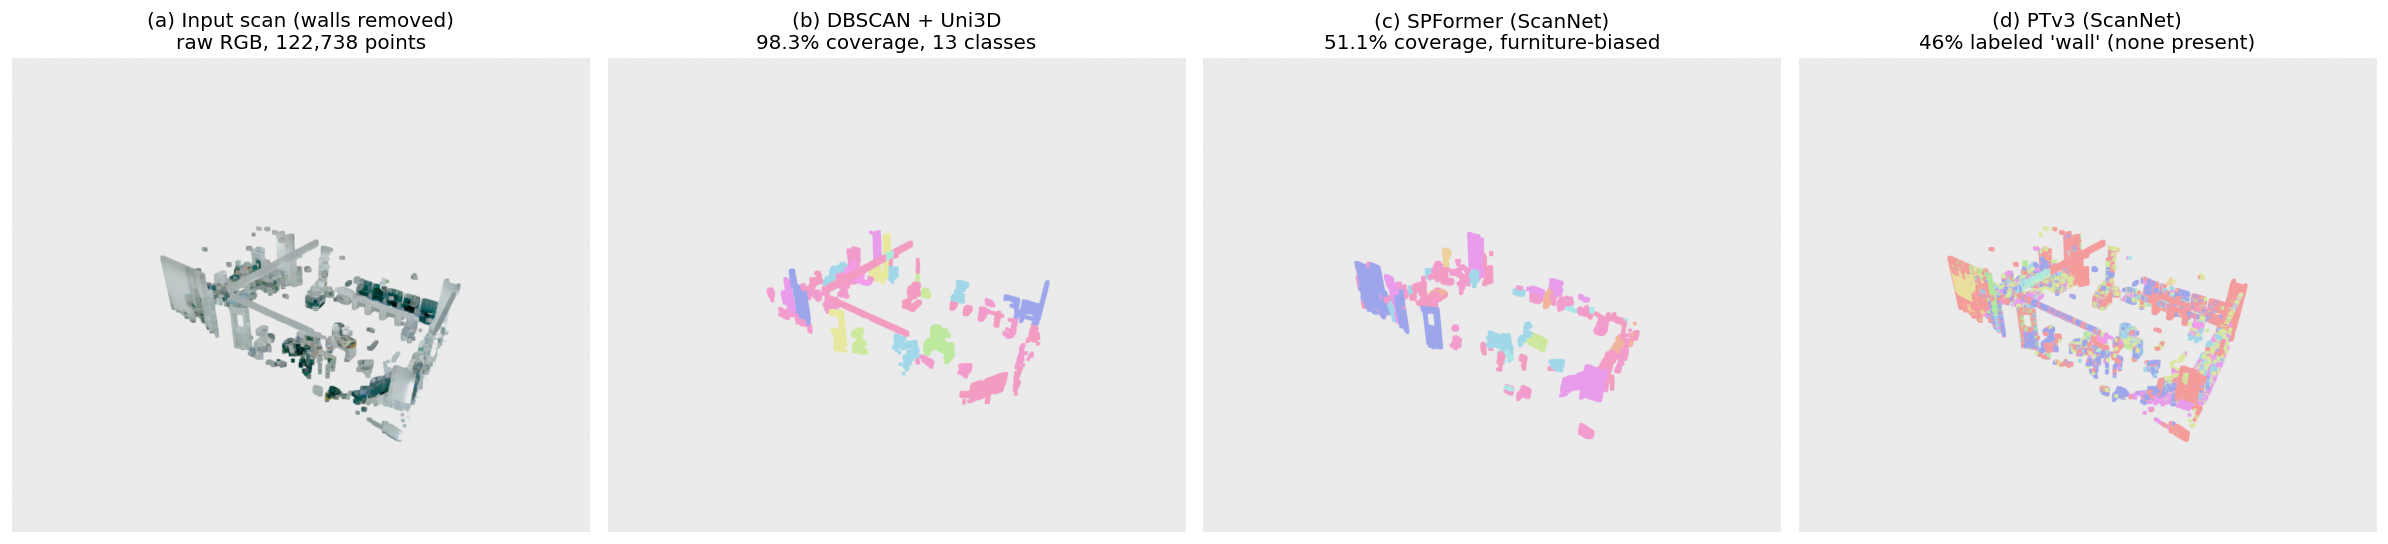
\includegraphics[width=\textwidth]{figures/fig6_2.png}
  \caption{Object segmentation on the test-room scan. (a)~The input cloud after
  wall removal (raw RGB). (b)--(d) are colored by predicted class: (b)~the
  geometric DBSCAN clustering with Uni3D labels covers the scene with coherent
  objects across 13 classes; (c)~SPFormer (ScanNet closed-set) assigns only
  about half of the points and biases toward indoor-furniture classes;
  (d)~PTv3 (ScanNet semantic) labels nearly half of the points \texttt{wall}
  although the walls were removed.}
  \label{fig:segcompare}
\end{figure}

\subsection{Repeatability and Remnant Filtering}
\label{subsec:exp-repeat}

Running the full pipeline twice from the same E57---including ten-plane
structure removal---reproduces every cluster byte-identically on both main
scenes (hash-verified). To probe robustness beyond one software stack, the
backbone was packaged into a version-pinned container and re-run under a
deliberately different environment (different glibc and Python patch
versions): all 81 retained robot-hall clusters remain byte-identical to the
native run. Running the same container on a second machine with a different
CPU vendor and microarchitecture (an Intel Core i9-13900H laptop versus the AMD
reference workstation) reproduces the identical per-cluster checksums---the
determinism claim holds across operating environments and x86-64 CPU vendors
under the pinned library set; bit-level reproducibility across instruction-set
architectures is not claimed. The structure-remnant filter of
Section~\ref{subsec:decomposition} removed all fourteen owner-confirmed
ceiling-soffit phantoms (seven per scene: showroom $45\rightarrow38$, robot
hall $88\rightarrow81$) while leaving every retained cluster unchanged. Before
the filter, these phantoms produced confidently verified fictions (keyboard
panels, handrails) that survived multi-view voting, since every view showed the
same wall-colored slab; detecting structure remnants geometrically, upstream of
semantics, proved more reliable than asking the verifier to doubt itself.

\subsection{Parameter Sensitivity and Coverage Stress}
\label{subsec:exp-params}

A 36-combination sweep (giant-split footprint $\times$ DBSCAN $\varepsilon$
$\times$ minimum points) shows a stable plateau at footprint 2.0--2.5~m:
instance recall degrades at 3.0~m as neighbors merge and at 1.5~m as equipment
shatters. Because scoring a sweep against the operating point's own
decomposition would be circular, every combination was re-scored against an
independent object-level reference: the owner-audited inventory in a
membership-independent form (all clean-cloud points falling inside each
owner-audited oriented box). On the robot hall (42 reference objects) the
min-points-100 band is a broad plateau and the operating point (2.5~m / 0.30 /
100) sits at the grid maximum (recall 0.952). On the showroom, the audit
surfaced an error, which is reported plainly: against the genuinely audited 57-object
inventory no grid combination of the base clustering exceeds recall 0.33---the
audited granularity of that scene is produced by the split-refinement stage,
not by any base-DBSCAN setting---so the parameter-robustness claim rests on the
non-circular robot-hall table. Two further perturbations bound the geometric
operating regime: voxel size is part of a jointly calibrated triple with
$(\varepsilon,\mathrm{min\_points})$ (at 3~cm the backbone recovers 42/42
reference objects, but 2~cm collapses recall to 0.36 as 22 objects merge and
5~cm to 0.33 as small objects starve), and seeded per-point Gaussian noise at
$\sigma=5$~mm---the scale of the scanner's real bundle error---drops recall to
0.48, with the 5~cm RANSAC inlier band saturating first. The T3 epoch supplied
a coverage stress case: at 99.6\% coverage, inter-object gaps close and DBSCAN
chains 120~K points (41\% of the clean cloud) into one $10.4\times9.6$~m
mega-cluster that survives the giant-split; refinement recovers little of the
resulting diff inflation, which is itself informative: about 88\% of that
epoch's absences reflect genuine scene change, not segmentation artifacts.

\subsection{Corrective Layers in Operation}
\label{subsec:exp-corrective}

Two T3 clusters that survived every upstream filter are \emph{diffuse webs}:
95~K and 13~K points spread over 80 and 12~m$^2$ at a 2D occupancy fill below
0.3, connected at $\sim$1.8~cm point spacing at any usable $\varepsilon$. The
diffuseness-gated re-split resolves them by \emph{cause} instead of size:
points hugging the exploration-grid wall line are structure noise ($\sim$70\%
of the 95~K-point residual), out-of-room bleed-through accounts for another 7\%,
and the remainder is re-clustered by occupancy-core erosion and split at the
support plane. The owner's ground truth for the largest compound---``a robot
arm on a desk, part of a mobile robot, wall noise''---is recovered exactly.
Applied to a 6.2~m wall-flush cluster that verification had confidently labeled
\texttt{electrical cabinet} (0.83), the wall-compound gate recovers the owner's
inventory at unit granularity: nine of the ten owner-confirmed monitor units,
the desk beneath them, and, from the off-wall remainder, a wheelchair robot;
unit boundaries are approximate because the dark screens return few points,
so the result is claimed as unit-level recall, not precise per-unit
segmentation. The structure-condition ensemble recovered two multi-meter
tables that exist in \emph{no} single-condition segmentation of the production
path---they appear only when walls are left in place---raising in-room recall
by four real objects ($\sim$8\%) as a standalone pass. The fusion also
quantifies label fragility: only 10 of 37 re-found objects keep the same label
across conditions, and cross-condition \emph{voting} corrected nothing, because
the verifier's biases are correlated across conditions (both recovered tables
were unanimously mis-verified as conveyor belts in every condition). Under a
pre-specified adoption rule, Point-SAM~\cite{zhou2024pointsam} separated 3/6
flagged merged clusters with sub-cluster labels reaching 9/11 versus 5/11 for
their parents, but automatic candidate selection also produced 2/6 false
positives, so it is retained only as an optional, manually triggered diagnostic
refinement (Figure~\ref{fig:baselines}).

\begin{figure}[!htb]
\centering
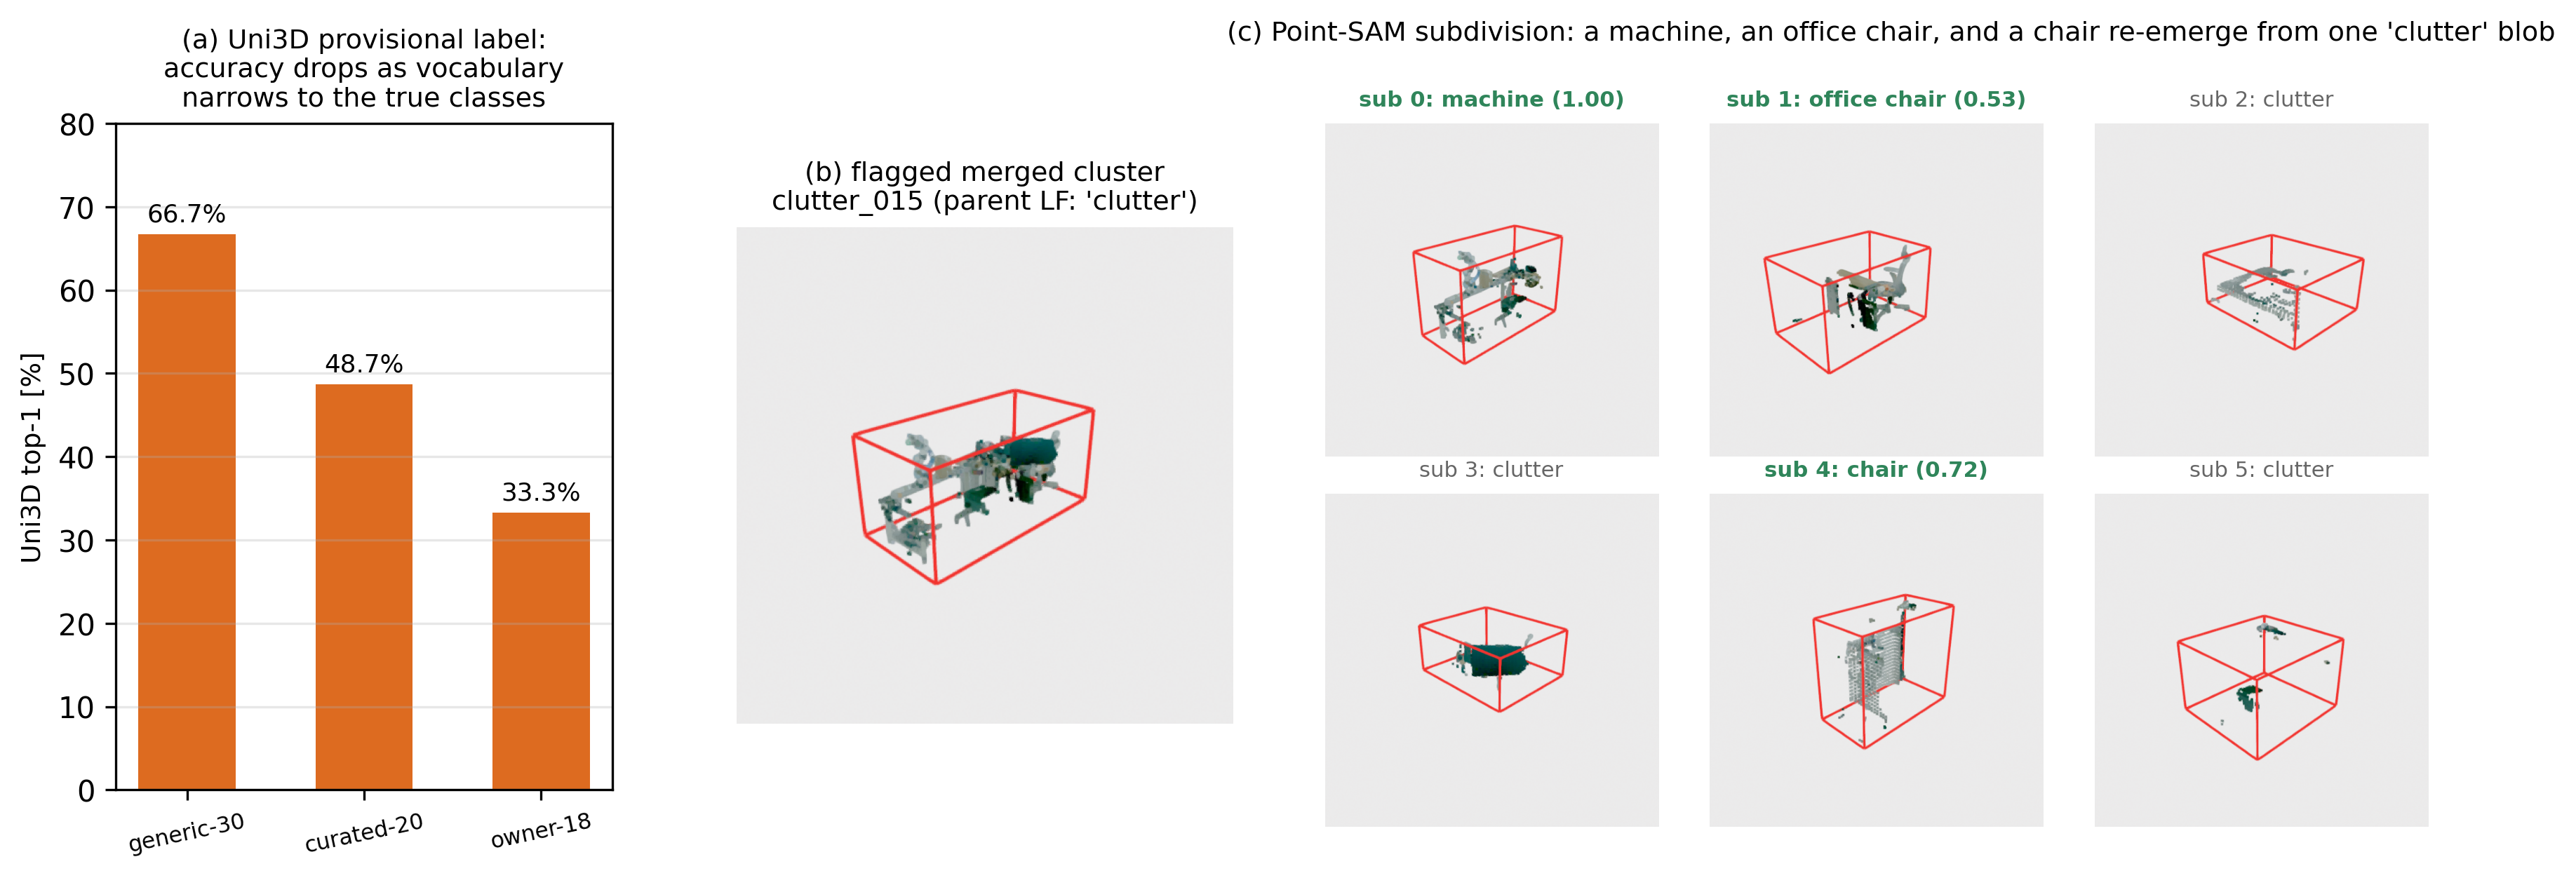
\includegraphics[width=0.95\linewidth]{figures/ele_fig13_pointsam_uni3d.png}
\caption{Learned components used as bounded tools. (a)~The Uni3D provisional
label degrades as the vocabulary narrows to the deployment's true classes
(Section~\ref{sec:exp-ablation})---why it is treated as untrusted context.
(b,c)~Conditional Point-SAM refinement of a flagged merged cluster: a machine,
an office chair, and a chair re-emerge from a single \texttt{clutter} blob,
each re-verified independently.}
\label{fig:baselines}
\end{figure}

\section{Verification: Multi-View Fusion and Escalation}
\label{sec:exp-verify}

\subsection{Multi-View Fusion Study}
\label{subsec:exp-multiview}

The first verification study, on the 57-object showroom decomposition, asks
how a VLM should consume multiple rendered views. Six configurations are
compared: a classifier-only reference, a $2\times2$ design over view count
(1 vs.\ 4, early fusion) and render/prompt generation (sparse renders with a
base prompt vs.\ dense renders with the guardrail prompt), and a sixth that
differs from four-view early fusion only in the fusion rule
(Table~\ref{tab:configs}). Labels are graded by two
independent references: a render audit by two of the authors against the dense
four-view renders and the measured dimensions, and the on-site inventory of the
facility operator by physical inspection, without reference to the render
audit. Audit-versus-inventory agreement is 79--95\% over the five VLM
configurations (Cohen's $\kappa$ 0.53--0.89). Three findings stand out
(Figure~\ref{fig:accuracy}).

\begin{table}[htbp]
\caption{Final type labels (57 showroom objects) under both references. Render
audit: C/P/W = correct / plausible / wrong, strict = C, lenient = C+P.
Inventory: strict matches on all 57 objects and on the 36 confirmed
non-structure objects. Source: ICTC~2026~\cite{kim2026ictc}.}
\label{tab:configs}
\centering
\begin{tabular}{l c c c c c c c}
\toprule
 & \multicolumn{5}{c}{\textbf{Render audit}} & \multicolumn{2}{c}{\textbf{Inventory}} \\
\textbf{Configuration} & C & P & W & strict & lenient & 57 & 36 \\
\midrule
Uni3D only (no VLM)            & 28 & 5  & 24 & 49\% & 58\% & 33 & 28 \\
1 view, base prompt, sparse    & 34 & 12 & 11 & 60\% & 81\% & \textbf{44} & \textbf{33} \\
4 views early fusion, sparse   & 28 & 10 & 19 & 49\% & 67\% & 34 & 27 \\
1 view, guardrails, dense      & 29 & 11 & 17 & 51\% & 70\% & 32 & 29 \\
4 views early fusion, dense    & 26 & 12 & 19 & 46\% & 67\% & 30 & 23 \\
4 views late fusion, dense     & 28 & \textbf{14} & \textbf{15} & 49\% & \textbf{74\%} & 34 & 28 \\
\bottomrule
\end{tabular}
\end{table}

\begin{figure}[!htb]
\centering
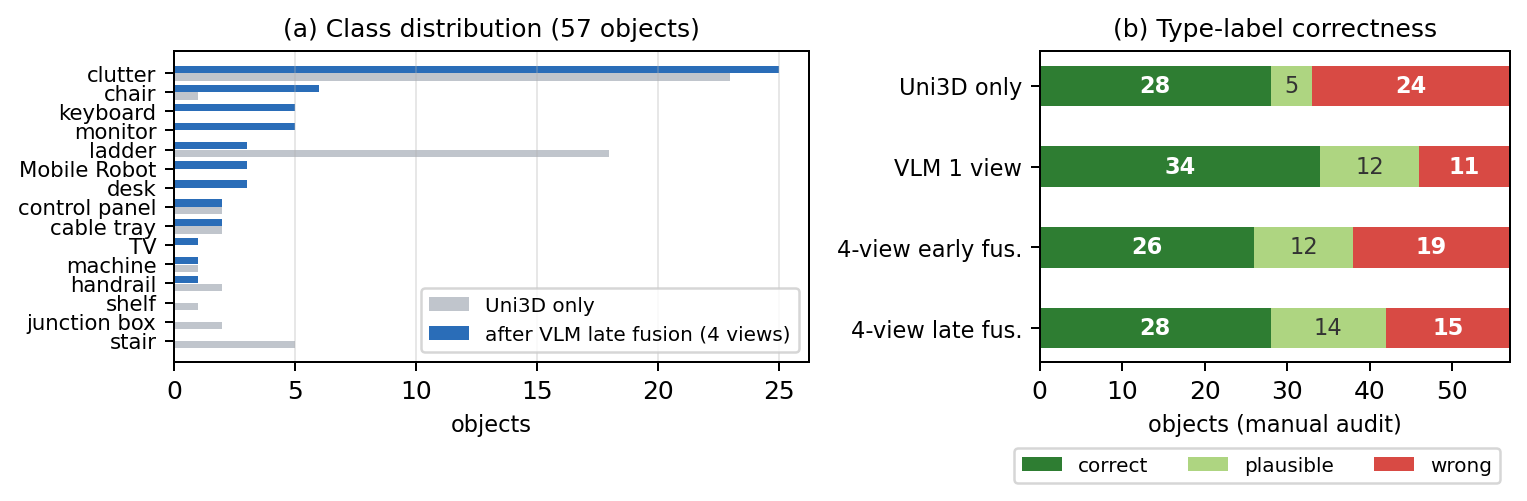
\includegraphics[width=0.95\linewidth]{figures/ictc_fig_accuracy.png}
\caption{Effect of VLM verification on the 57-object showroom scene.
(a)~Class distribution, classifier-only vs.\ after late fusion: implausible
\emph{ladder}/\emph{stair} populations are redistributed to displays and
furniture. (b)~Render audit: early fusion degrades single-view accuracy; late
fusion is the strongest multi-view strategy (15 wrong labels vs.\ 19 for
early fusion).}
\label{fig:accuracy}
\end{figure}

\emph{Early fusion hurts.} Feeding four sparse views into one prompt dropped
strict accuracy from 60\% (single view) to 49\%: extra oblique speckle views
encouraged over-committed readings, e.g., two electrical cabinets confidently
relabeled \emph{chair}; denser renders and the guardrails did not close the
gap, and the inventory confirms the direction. \emph{Late fusion is the
strongest multi-view strategy, but not the best configuration.} Judging each
view independently and voting beats early fusion on every measure (15 vs.\ 19
wrong labels, 74\% vs.\ 67\% lenient; 34 vs.\ 30 inventory matches) because a
contaminated view is outvoted, but it does not overtake the best single
canonical view (44/57 inventory matches, 77\%, versus 34/57): on sparse point
clouds extra views add noise faster than evidence, and the vote spends much of
its gain on caution. Late fusion is therefore claimed as the safer multi-view
rule, not as an accuracy gain over a well-chosen single view. \emph{Vote
unanimity is a free precision signal.} 17 of 57 objects received identical
labels from all four views; 16 of those (94\%) were audited correct and match
the inventory, versus 30\% (audit) or 18/40 (inventory) among split-vote
objects. Two re-runs of the late-fusion protocol bound the verifier's sampling
variance: accuracy on the 36 confirmed objects was 28, 27, and 27 across three
runs, and unanimity precision 16/17, 20/21, and 19/20 (94--95\%). Render
density produced the study's starkest warning: dense renders made four
dotted-grid panels look so convincingly like keyboards (per-view confidence up
to 0.97) that the label passed the render-based audit---only the inventory
revealed them to be ceiling-soffit remnants. A label that fools both the VLM
and a human at the same renders was still caught by vote splits, the strongest
argument for gating, and the incident motivated the structure-remnant filter.
On the late-fusion output, the implicit prompt marked 6 of 57 objects as key
objects (control panels, a large machine, mobile robots, and a wall display)
and 50 as movable; Figure~\ref{fig:ictccards} shows two completed records.

\begin{figure}[!htb]
\centering
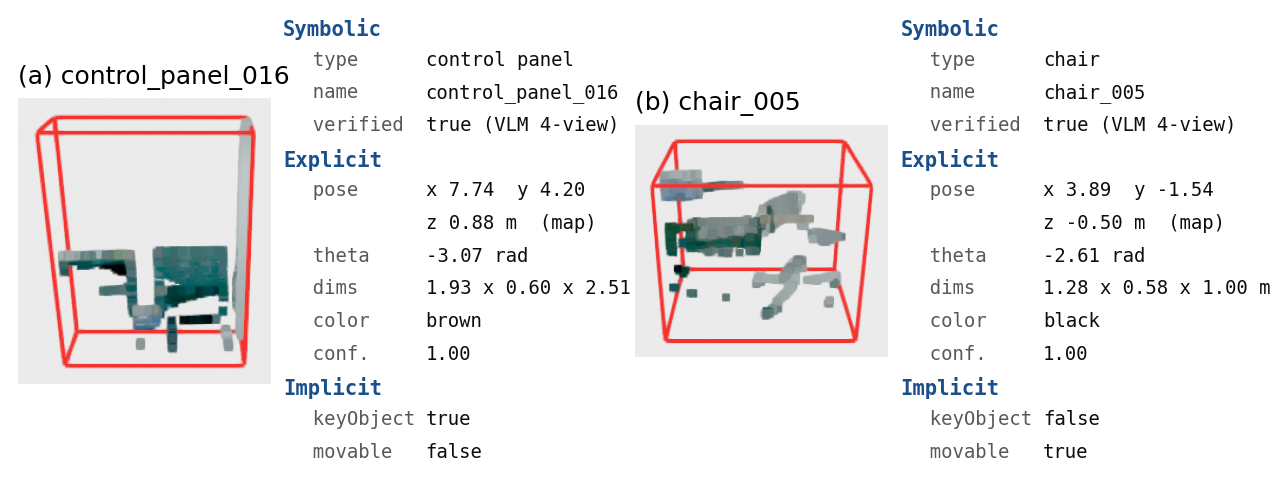
\includegraphics[width=0.95\linewidth]{figures/ictc_fig_cards.png}
\caption{Completed TOSM semantic-object records (dense render with symbolic /
explicit / implicit fields) as serialized into the VDA~5050-style message.
(a)~A control panel, unanimously verified and marked as a fixed key landmark.
(b)~An office chair corrected from \emph{stair}, movable and not a landmark.}
\label{fig:ictccards}
\end{figure}

\subsection{Escalation, Tiers, and Threshold Sensitivity}
\label{subsec:exp-escalation}

The escalation mechanism of Section~\ref{subsec:escalation} is evaluated on
both main scenes (Table~\ref{tab:verification}). Escalation lifts
confirmed-ground-truth accuracy from 77.8\% to 88.9\% on the showroom and from
78.1\% to 84.4\% on the robot hall (lenient: $76.2\%\rightarrow83.3\%$,
$n=42$), recovering 5 and 3 split-vote objects while regressing 1 and 0---a
consistent observed improvement across both scenes, though at these
sample sizes the paired contrast does not reach conventional significance
(exact McNemar $p=0.219$ and $p=0.25$), which the Wilson intervals make
explicit. Escalation adds 232 and 208 calls per scene at $\sim$\$0.009 per
call (Figure~\ref{fig:esccost}). The tier structure justifies the gating:
unanimous and escalated tiers reach 88.9--100\% precision, while the
unverified residue is 40--60\%---exactly the content the query interface must
demote. A repeat of the showroom run under identical settings bounds the
verifier's run-to-run variance at about $\pm3$ points. Verification yield
tracks scan quality: the manual scan leaves 47\% of objects unverified versus
24\% for exploration scans, and re-processing the T3 scan from a single setup
(1/6 coverage) drops the verified tier from 75.6\% to 56.6\% on identical
geometry---coverage buys verifiability, which ties Part~B back to Part~A.

\begin{table}[htbp]
\centering
\caption{Verification accuracy against confirmed ground truth, and per-tier
precision. Accuracy rows are over confirmed GT ($n=36$/32); trigger rates and
tier counts are over all GT-scored clusters (50 showroom / 51 robot hall).
Source: \emph{Electronics}~\cite{kim2026electronics}.}
\label{tab:verification}
\begin{tabular}{l c c c c}
\toprule
 & \multicolumn{2}{c}{\textbf{Showroom ($n=36$)}} & \multicolumn{2}{c}{\textbf{Robot hall ($n=32$)}} \\
 & base-4 & escalated & base-4 & escalated \\
\midrule
Accuracy & 77.8\% & \textbf{88.9\%} & 78.1\% & \textbf{84.4\%} \\
95\% Wilson CI & 61.9--88.3 & 74.7--95.6 & 61.2--89.0 & 68.2--93.1 \\
Recovered / regressed & \multicolumn{2}{c}{5 / 1} & \multicolumn{2}{c}{3 / 0} \\
Escalation trigger & \multicolumn{2}{c}{58\% (29/50)} & \multicolumn{2}{c}{51\% (26/51)} \\
\midrule
Unanimous precision & \multicolumn{2}{c}{100\% (19/19; 21 unan.)} & \multicolumn{2}{c}{94.4\% (17/18; 25 unan.)} \\
Escalated precision & \multicolumn{2}{c}{100\%} & \multicolumn{2}{c}{88.9\%} \\
Unverified precision & \multicolumn{2}{c}{60\%} & \multicolumn{2}{c}{40\%} \\
\bottomrule
\end{tabular}
\end{table}

\begin{figure}[!htb]
\centering
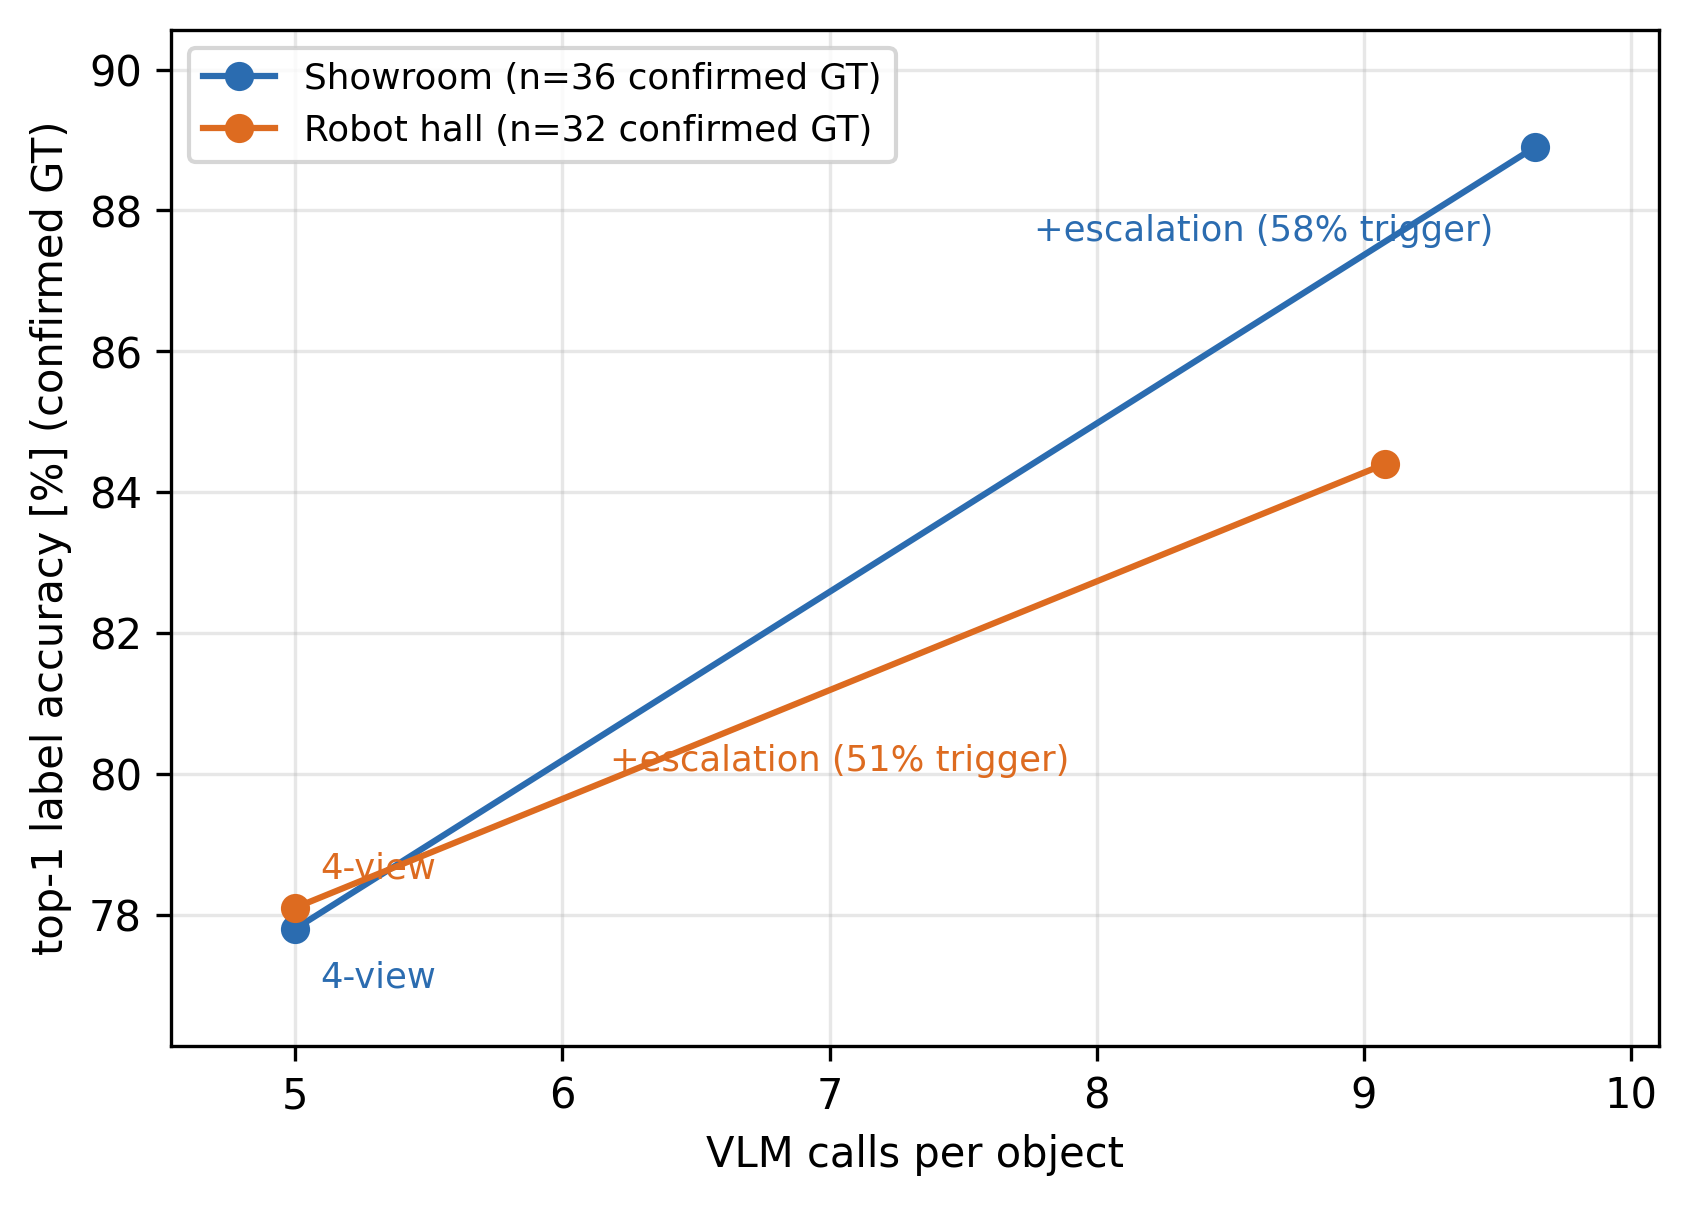
\includegraphics[width=0.85\linewidth]{figures/ele_fig6_escalation_cost.png}
\caption{Escalation accuracy--cost curves for both scenes.}
\label{fig:esccost}
\end{figure}

Precision alone understates what gating costs, so Table~\ref{tab:tierrf}
completes the tier picture with recall and $F_1$. The combined verified tier
reaches recall 0.722/0.781 on the two industrial scenes ($F_1$ 0.839/0.847)
but only 0.250 on the cafeteria, where the gate abstained on half of the
confirmed objects---the stress scene's segmentation failures surface as
recall, not as precision. Because the 0.6 share threshold gates status only,
its effect can be quantified exactly by re-scoring the stored votes at
alternative thresholds: sweeping 0.40--0.90 shows 0.6 sitting on a plateau
rather than a cliff, with $F_1$ maximized on a broad 0.45--0.65 band on both
industrial scenes and every 0.05 step moving at most one or two objects, so the
a priori 0.6 is retained rather than tuned post hoc.

\begin{table}[htbp]
\centering
\caption{Per-tier precision, recall, and $F_1$ on confirmed ground truth
(synonym-tolerant). The unverified row is the abstention tier.}
\label{tab:tierrf}
\small\setstretch{1.15}
\begin{tabular}{l l r r r r r}
\toprule
\textbf{Scene} & \textbf{Tier} & $n$ & $n_{\mathrm{conf}}$ & Prec. & Rec. & $F_1$ \\
\midrule
Showroom & verified (unanimous) & 21 & 19 & 1.000 & 0.528 & 0.691 \\
 & verified\_escalated & 8 & 7 & 1.000 & 0.194 & 0.326 \\
 & combined verified & 29 & 26 & 1.000 & 0.722 & 0.839 \\
 & unverified (abstained) & 21 & 10 & 0.600 & 0.167 & 0.261 \\
\midrule
Robot hall & verified (unanimous) & 25 & 18 & 0.944 & 0.531 & 0.680 \\
 & verified\_escalated & 16 & 9 & 0.889 & 0.250 & 0.390 \\
 & combined verified & 41 & 27 & 0.926 & 0.781 & 0.847 \\
 & unverified (abstained) & 10 & 5 & 0.400 & 0.062 & 0.108 \\
\midrule
Cafeteria & verified (unanimous) & 8 & 7 & 0.571 & 0.200 & 0.296 \\
 & verified\_escalated & 6 & 3 & 0.333 & 0.050 & 0.087 \\
 & combined verified & 14 & 10 & 0.500 & 0.250 & 0.333 \\
 & unverified (abstained) & 11 & 10 & 0.200 & 0.100 & 0.133 \\
\bottomrule
\end{tabular}
\end{table}

\subsection{Error Taxonomy and Class-Level Breakdown}
\label{subsec:exp-errors}

Four recurring error classes emerged (Figure~\ref{fig:taxonomy}):
(a)~\emph{structure-remnant phantoms}---soffit bands verified as keyboards,
eliminated upstream by the remnant filter; (b)~\emph{unanimous-but-wrong}---a
hanging chain unanimously verified as a door handle, partition fragments as
chairs, and at T3 a residual 7.4~m wall segment escalation-verified as a
staircase whose phantom label then propagated into a place name
(\texttt{staircase\_landing}), showing that place naming is verifier-bounded
too; a third case is the mirror image, in which the room's large wall-mounted
TV was geometrically detected yet left \texttt{unverified} while a small
co-located cluster was verified as a fire extinguisher the owner refuted;
(c)~\emph{clutter absorption}---a disassembled robot, a poster stand, and a
low-reflectance floor fan (674 points) each unanimously verified as
\texttt{clutter}: geometrically detected, semantically flattened; and
(d)~\emph{render ambiguity} $\rightarrow$ \texttt{unverified}, the intended
failure mode. Classes (b) and (c) motivate reporting verification as tiered
evidence rather than truth. Table~\ref{tab:classdist} disaggregates every
scene's ground truth into class families: robots are the worst family
everywhere they occur (0/4, 0/3, and 0/8 correct across the three
robot-bearing sets)---absorption, not misperception, since most land in
\texttt{clutter} or abstain---and displays and fixtures abstain heavily on the
showroom, exactly the render-ambiguous shapes the taxonomy predicts.

\begin{figure}[!htb]
\centering
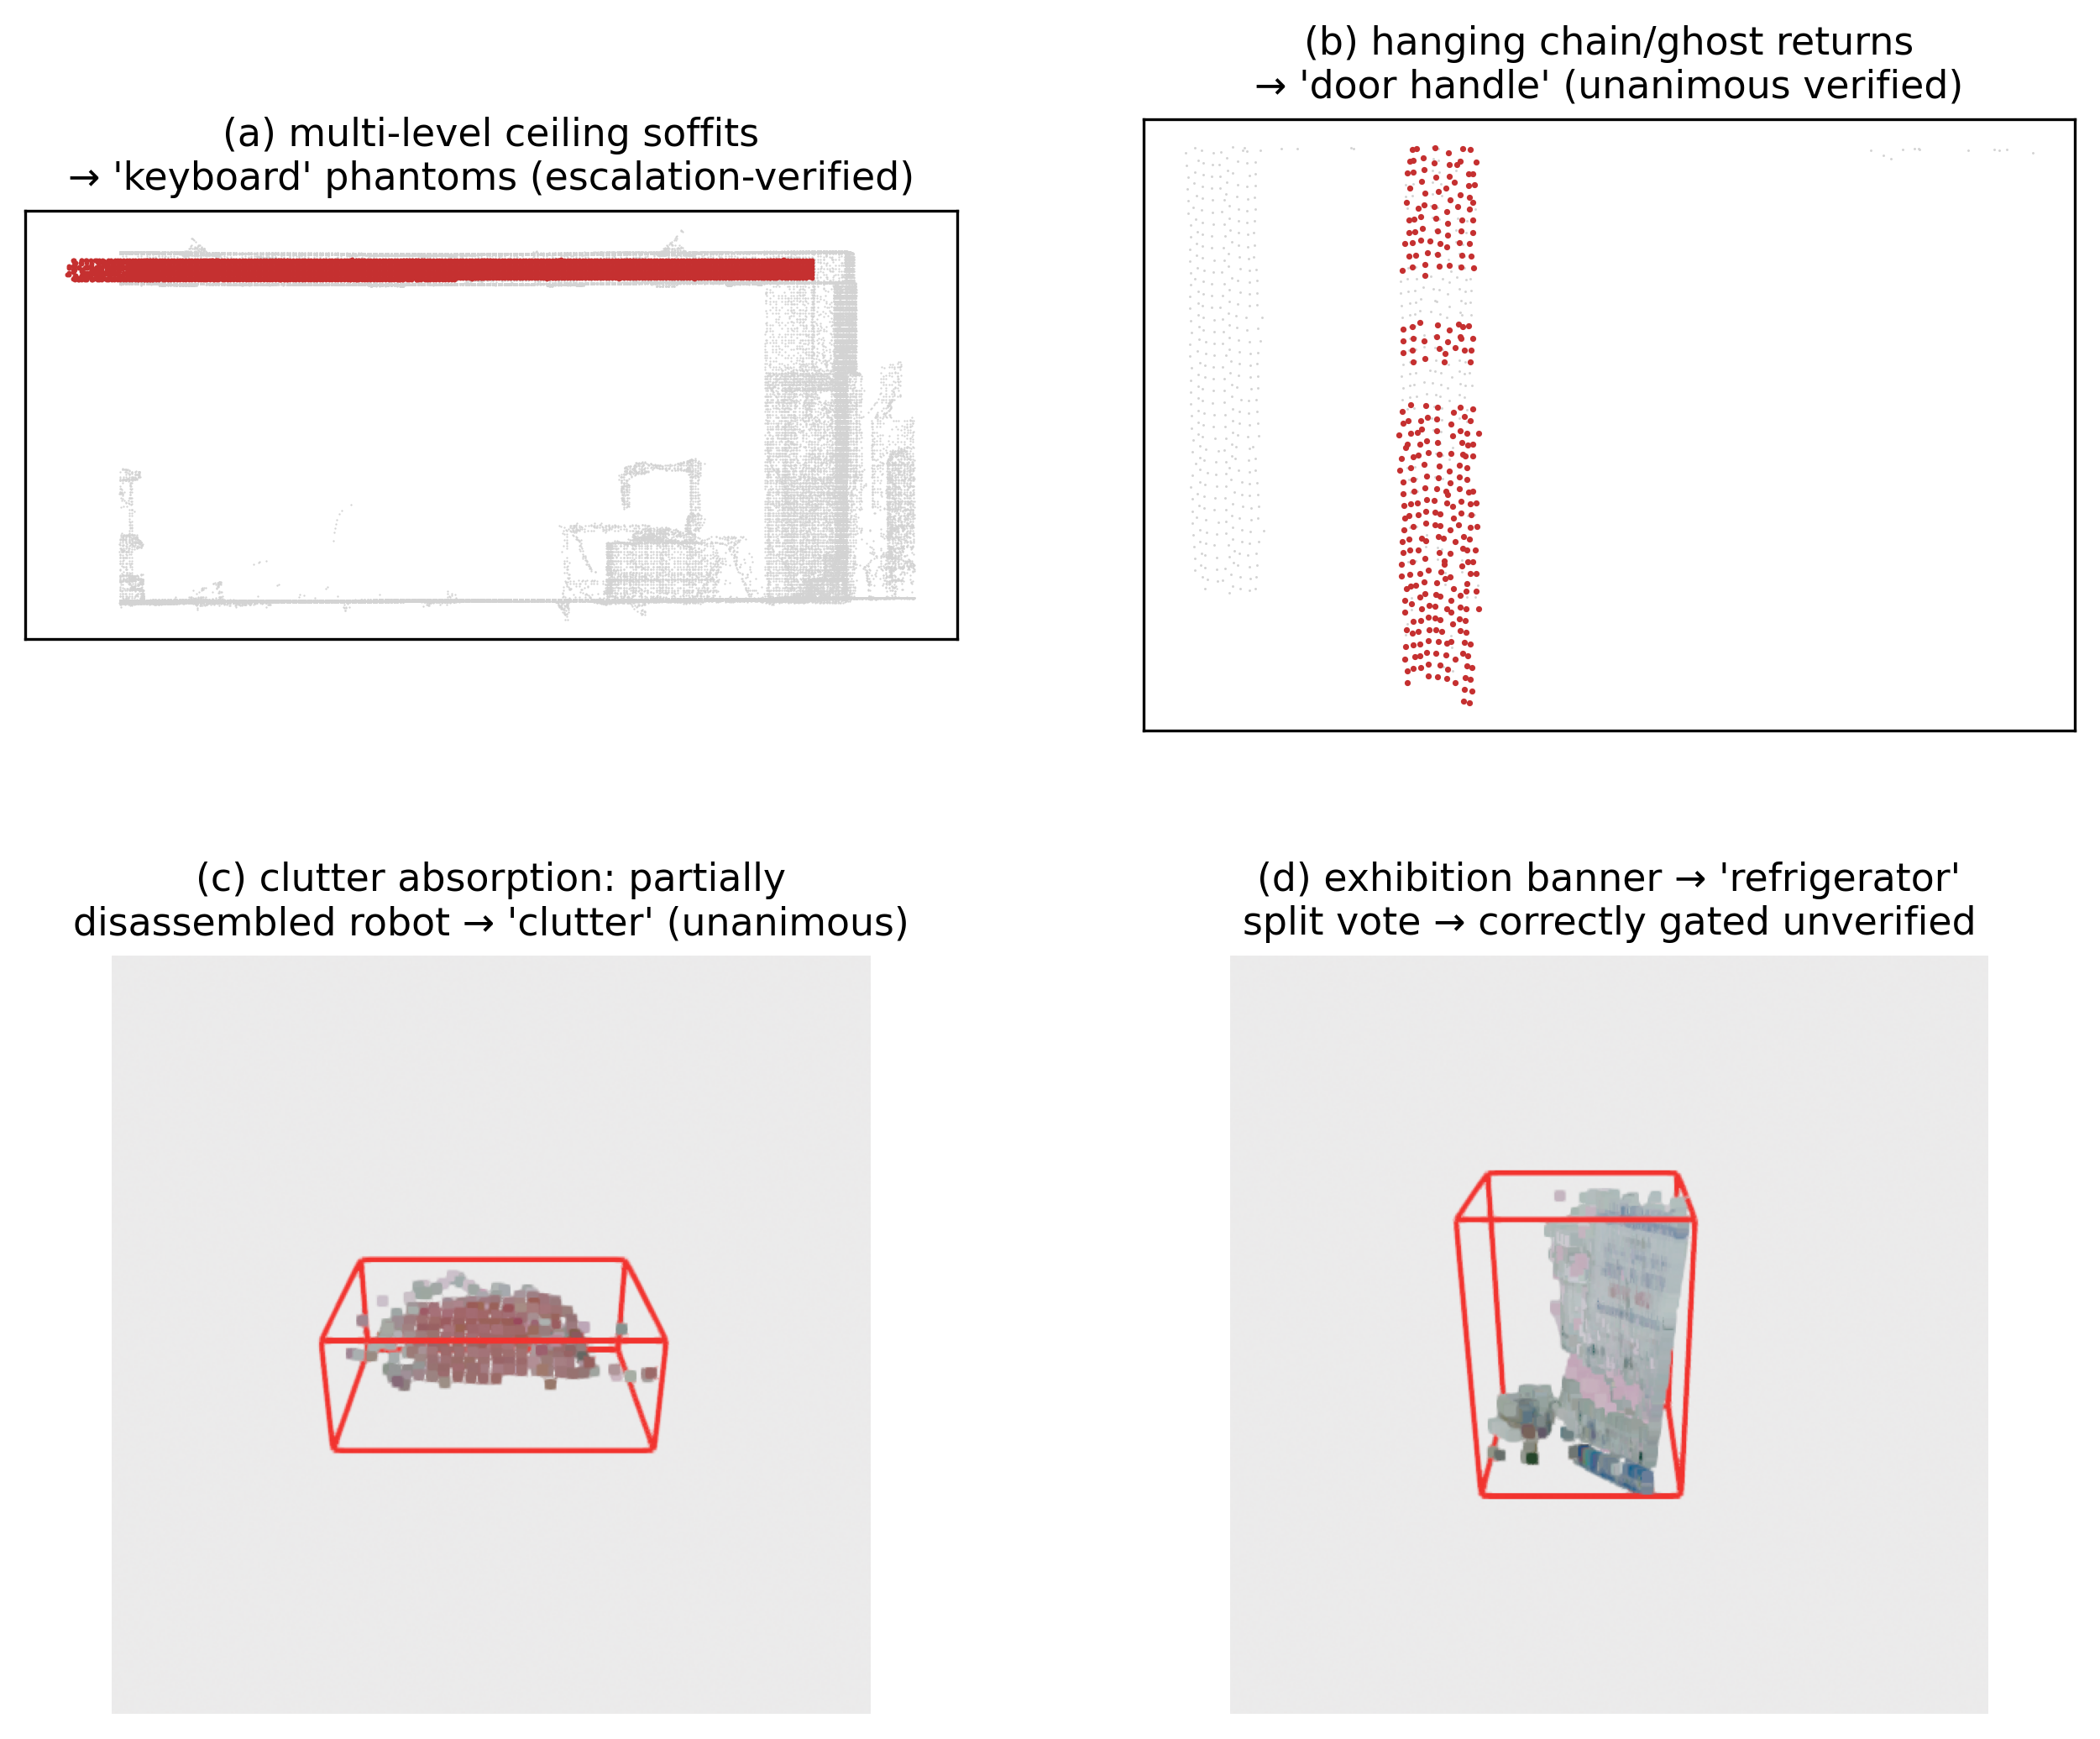
\includegraphics[width=0.9\linewidth]{figures/ele_fig10_error_taxonomy.png}
\caption{Verification error taxonomy: remnant phantom, unanimous-but-wrong,
clutter absorption, render ambiguity.}
\label{fig:taxonomy}
\end{figure}

\begin{table}[htbp]
\centering
\caption{Ground-truth object classes per scene, grouped into families, with
each object's verification outcome in the canonical run. ``Filtered'' =
excluded before scoring (structure artifact or out of room scope).}
\label{tab:classdist}
\small\setstretch{1.15}
\begin{tabular}{l l r r r r r}
\toprule
\textbf{Scene} & \textbf{Family} & GT & Corr. & Wrong & Unver. & Filt. \\
\midrule
Showroom (57-set) & seating & 5 & 4 & 1 & 0 & 0 \\
 & robots & 4 & 0 & 1 & 3 & 0 \\
 & displays/monitors & 5 & 0 & 0 & 5 & 0 \\
 & machines/electrical & 6 & 3 & 0 & 3 & 0 \\
 & furniture & 2 & 0 & 0 & 2 & 0 \\
 & fixtures & 6 & 0 & 0 & 6 & 0 \\
 & structure-noise & 7 & 0 & 0 & 0 & 7 \\
 & clutter/unknown & 22 & 20 & 0 & 2 & 0 \\
 & \emph{total} & 57 & 27 & 2 & 21 & 7 \\
\midrule
Robot hall (det) & seating & 5 & 4 & 0 & 1 & 0 \\
 & robots & 3 & 0 & 1 & 2 & 0 \\
 & displays/monitors & 1 & 0 & 0 & 0 & 1 \\
 & machines/electrical & 1 & 0 & 0 & 0 & 1 \\
 & furniture & 2 & 0 & 0 & 0 & 2 \\
 & fixtures & 8 & 3 & 1 & 4 & 0 \\
 & structure-noise & 8 & 0 & 0 & 1 & 7 \\
 & clutter/unknown & 53 & 25 & 7 & 2 & 19 \\
 & \emph{total} & 81 & 32 & 9 & 10 & 30 \\
\midrule
Cafeteria & seating & 10 & 1 & 4 & 5 & 0 \\
 & machines/electrical & 1 & 1 & 0 & 0 & 0 \\
 & furniture & 1 & 0 & 1 & 0 & 0 \\
 & fixtures & 5 & 0 & 1 & 4 & 0 \\
 & structure-noise & 3 & 0 & 0 & 0 & 3 \\
 & clutter/unknown & 8 & 4 & 2 & 2 & 0 \\
 & \emph{total} & 28 & 6 & 8 & 11 & 3 \\
\midrule
T3 re-scan (owner GT) & seating & 5 & 2 & 2 & 1 & 0 \\
 & robots & 8 & 0 & 6 & 2 & 0 \\
 & displays/monitors & 2 & 0 & 1 & 1 & 0 \\
 & machines/electrical & 4 & 0 & 4 & 0 & 0 \\
 & furniture & 4 & 0 & 3 & 1 & 0 \\
 & fixtures & 4 & 0 & 2 & 2 & 0 \\
 & structure-noise & 9 & 0 & 6 & 3 & 0 \\
 & clutter/unknown & 5 & 4 & 0 & 0 & 0 \\
 & \emph{total} & 41 & 6 & 25 & 10 & 0 \\
\bottomrule
\end{tabular}
\end{table}

\section{Owner Audit and Corrective Feedback}
\label{sec:exp-owner}

The preceding section measured what the pipeline believes; this one measures
what the room's occupant knows, and how that knowledge feeds back into the
graph. The room's occupant exhaustively labeled all 41 T3 clusters. Of the 31
verified-tier clusters, 6 were correct, 13 were real objects flattened to
\texttt{clutter}, 6 were structure-noise phantoms, 2 carried a wrong specific
label, and 3 were multi-object merges. The cause of the absorption is
identifiable: the room is a robotics testbed (mobile robots, manipulators,
charging stations, a disinfection robot), and none of these classes exist in
the classifier vocabulary. Three audit-driven mitigations follow (layers 4--5 of
Section~\ref{sec:corrective}). \emph{(i) Hybrid structure filter:} registering
every cluster against the exploration occupancy grid removes structure noise at
12/12 recall with 3 false positives (thin wall-flush real objects: a cabinet
leg, a poster stand); crucially, the wall-flush monitor bank survives, because
its 1.8~m height and per-segment depth separate it from the 3.2~m
floor-to-ceiling wall band that plane removal missed
(Figure~\ref{fig:structfilter}). \emph{(ii) Recovery re-verification:}
re-asking the verifier with \texttt{clutter} treated as unidentified plus a
candidate shortlist recovered 4 specific types at 4/5 precision; injecting
site vocabulary (robot classes) as candidates doubled recovery (9 correct) but
halved precision (8 wrong) through candidate anchoring---the TV became a
``conveyor belt'' when the shortlist ranked it first. \emph{(iii) Agreement
gating:} adopting a recovered label only when both passes agree, or when a
pass agrees with the cluster's own base label, yields five adoptions at 5/5
precision (two chairs, an office chair, a machine, and the TV) and resurrects
no owner-refuted phantom. Domain knowledge helps recall; only agreement makes
it safe. Refutations, corrections, and adopted labels were applied as a graph
revision through the same upsert mechanism as a re-scan: eight phantoms leave
the graph, five recovered types land, the TV becomes its region's key object,
the relation layer sheds nine noise-anchored edges, and re-deriving ring codes
heals the place layer end to end---the phantom-derived
\texttt{staircase\_landing} becomes \texttt{display\_briefing\_area}, the
keyboard-derived \texttt{workstation\_area} becomes \texttt{machine\_area},
and the seating region's recovered chairs turn
\texttt{cluttered\_seating\_area} into \texttt{seating\_area}. Owner feedback
thus propagates through all three layers of the model: object, relation, and
place.

\begin{figure}[!htb]
\centering
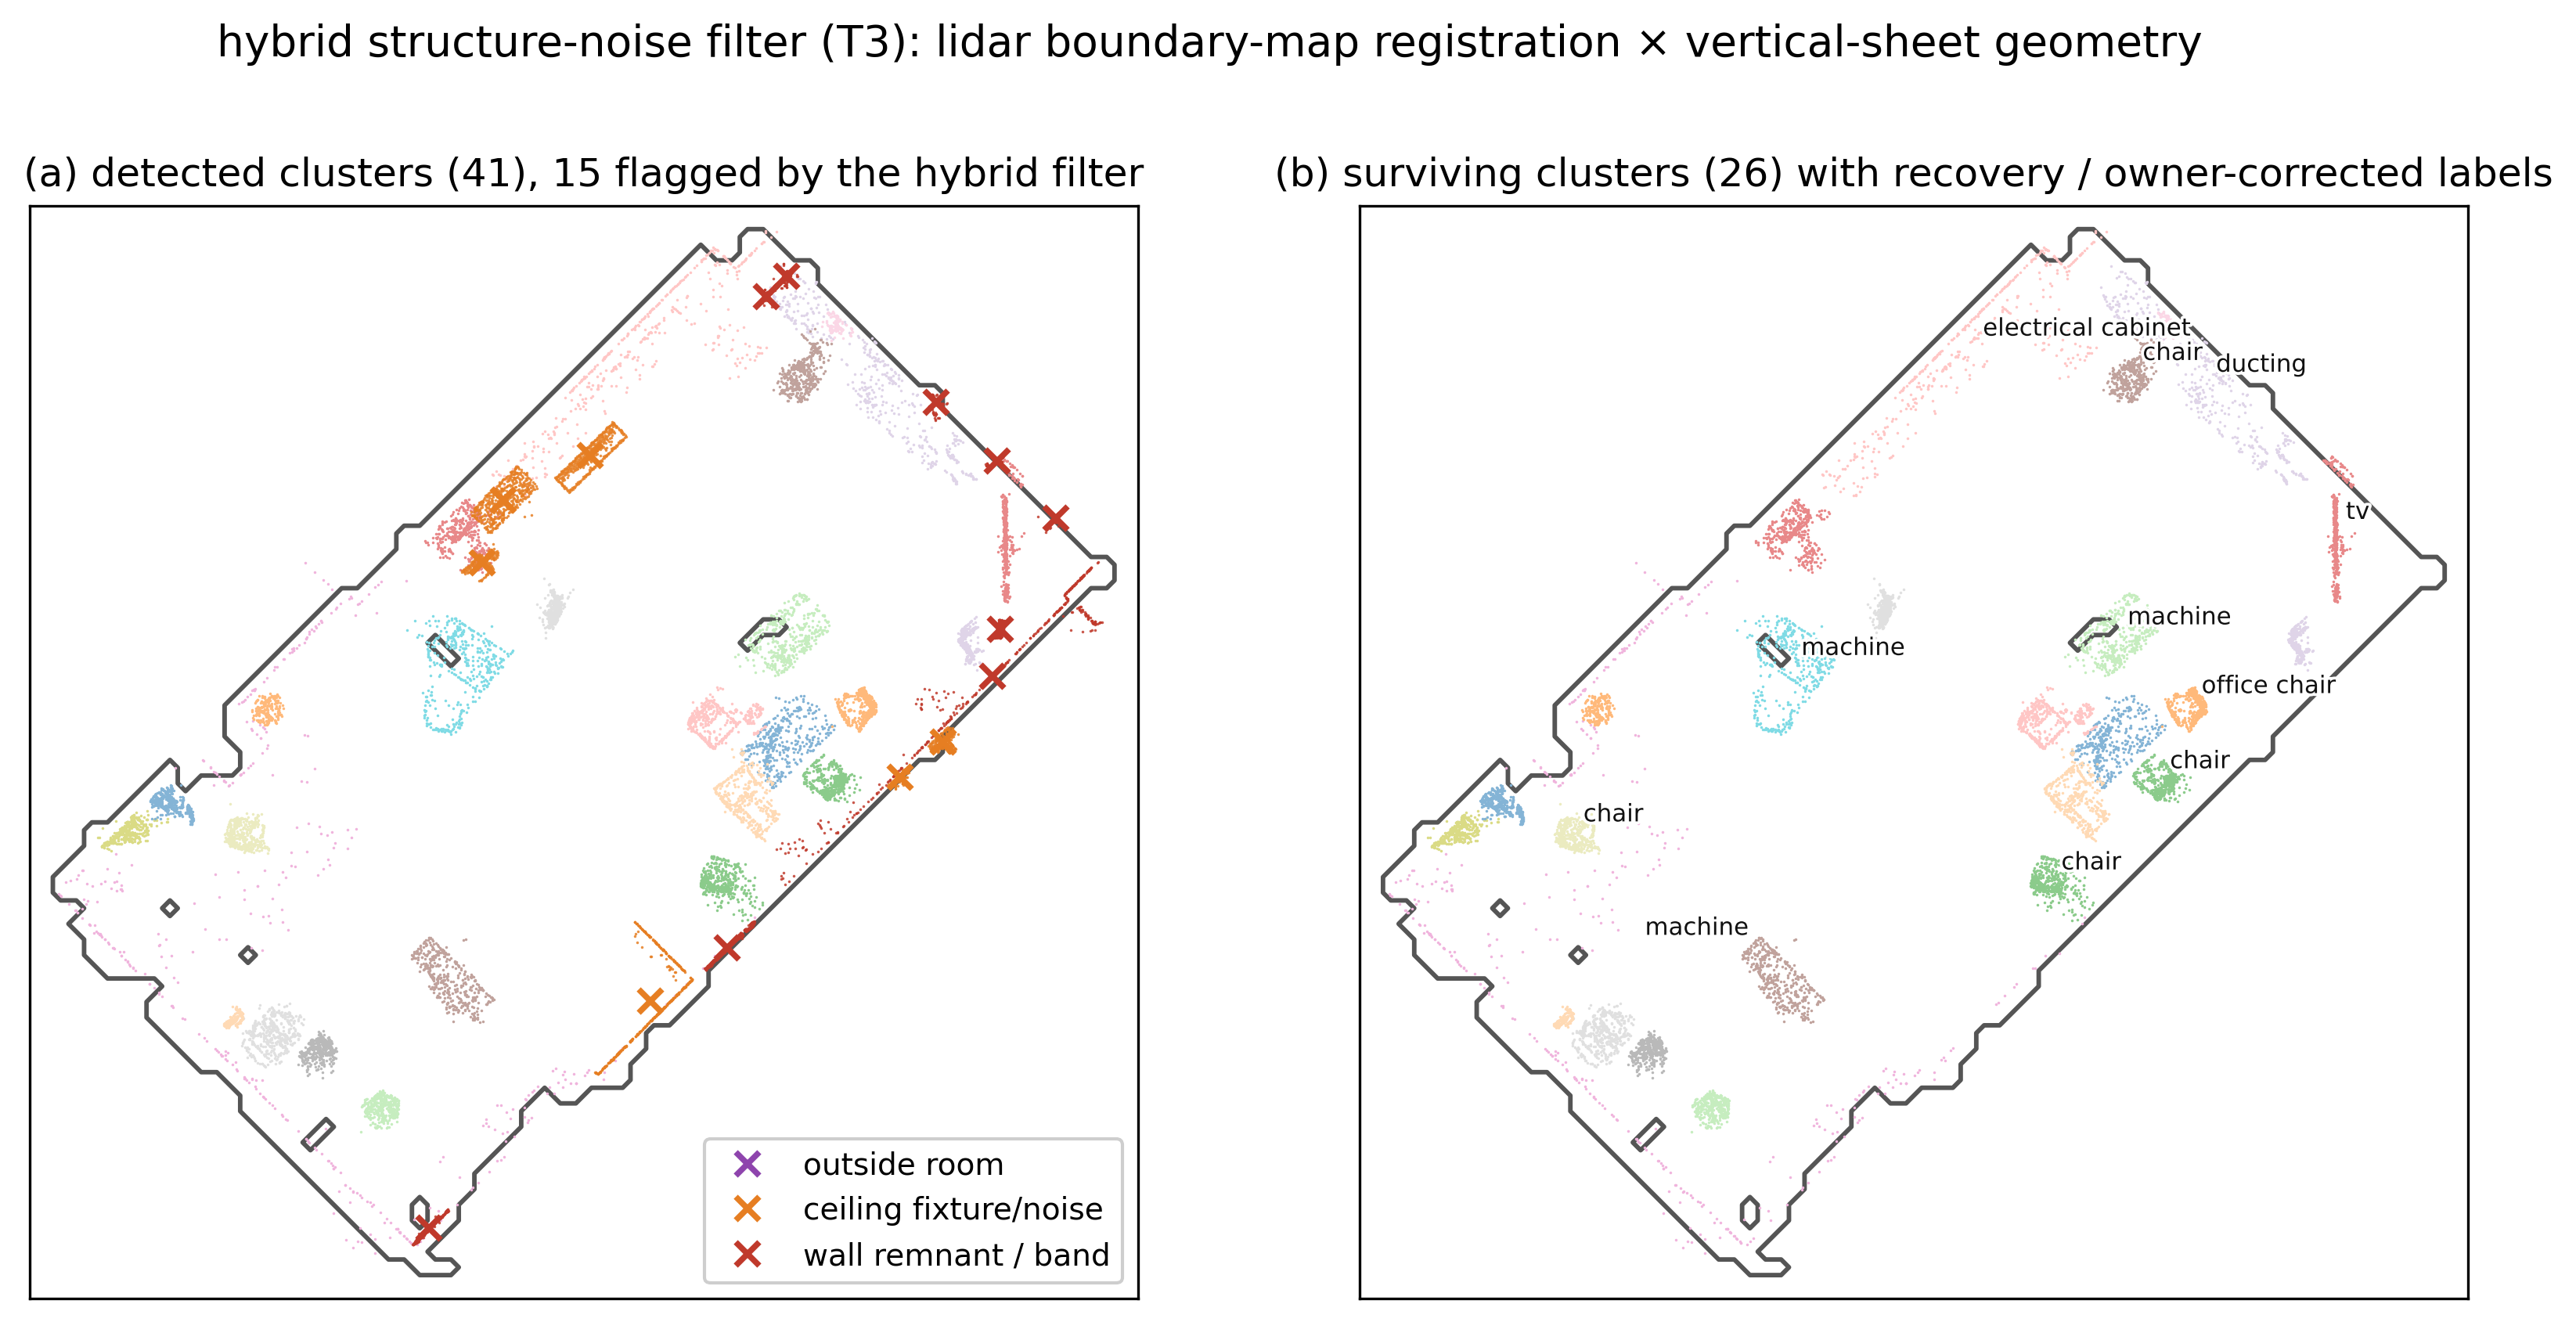
\includegraphics[width=\linewidth]{figures/ele_fig14_structure_filter.png}
\caption{Hybrid structure-noise filter on the T3 epoch. (a)~All 41 detected
clusters; the 15 flagged ones are colored by rule (wall remnant/band, ceiling
fixture/noise, outside the room boundary). (b)~The 26 survivors with recovery
and owner-corrected labels; the wall-flush monitor bank and wall-mounted
equipment survive.}
\label{fig:structfilter}
\end{figure}

Extending the audit loop through nine further revisions shows owner feedback
operating in all four directions the model supports. \emph{Restoration}: an
object the owner had refuted as absent was later declared present again (the
room changed between audits); a color-seeded carve at the owner-given corner
recovered a 319-point red cylinder that two-pass verification typed
\texttt{fire extinguisher}---the original failure was segmentation, not
classification, and owner ground truth is itself time-variant.
\emph{Refutation}: a raw-condition ensemble find was refuted as wall paint, the
halo around the hole left by the glossy black screen of the wall TV.
\emph{Label correction}: the correlated-bias tables and a poster stand were
corrected in place with the VLM verdict preserved in provenance.
\emph{Attribute correction}: wall-remnant clutter was marked immovable. The
live graph has accumulated thirteen revisions through the same mechanism, and
every transition, including the mistakes it corrects, is reconstructible from
node histories.

\section{Knowledge-Grounded Query Evaluation}
\label{sec:exp-query}

Four conditions are evaluated over identically constructed per-scene query
sets---48 items on the showroom, 32 on the robot hall (symbolic, explicit,
scene-level, and trap questions): (1)~\emph{LLM-only} (an unverified Stage-A
object dump, no verification), (2)~\emph{ungated KG}, (3)~\emph{verified-only
KG} (unverified nodes removed), and (4)~\emph{gated KG} (unverified retained
but structurally demoted). Each scene carries four trap questions about
objects that do not exist as labeled; on the showroom all four target
unverified-label phantoms, on the robot hall two target an unverified-label
phantom and two an \emph{escalation-verified} phantom, probing the gate's
verifier-quality bound. On the showroom (Table~\ref{tab:query},
Figure~\ref{fig:query}), grounding alone lifts accuracy from 52.1\% to 81.2\%
but blocks no traps; removing unverified content blocks all four traps at a
steep recall price (12 abstentions, 58.3\%); the gated condition is the balance
point---83.3\% with 3/4 traps blocked. The two leaks are mechanistically
distinct: on the showroom, one count-phrased trap slipped through the
quarantine itself, the model tallying a demoted node by reading its
\texttt{failedCandidateType} field; on the robot hall, the keyboard phantom is
escalation-verified, so it passes any status-based gate---gating is bounded by
verifier quality. The robot hall reproduces the ordering at lower absolute
levels because its end-to-end label errors propagate into every grounded
condition. At $n=48$/32 questions the gated-versus-ungated accuracy gap is a
single question on each scene, so the benchmark is diagnostic rather than
powered for significance; the case for gating rests on the mechanisms the
benchmark isolates---trap blocking, the abstention structure, and the direction
of the hallucination change---and on the mission-level consequences of
Section~\ref{sec:exp-missions}.

\begin{table}[htbp]
\centering
\caption{Query benchmark, four conditions. Acc.\ = accuracy, Hall.\ =
hallucination rate, Traps = trap questions blocked (of 4), Abst.\ =
abstentions. An abstention counts against accuracy but is not a hallucination.
Source: \emph{Electronics}~\cite{kim2026electronics}.}
\label{tab:query}
\small
\begin{tabular}{l c c c c c c c c}
\toprule
 & \multicolumn{4}{c}{\textbf{Showroom ($n=48$)}} & \multicolumn{4}{c}{\textbf{Robot hall ($n=32$)}} \\
\textbf{Condition} & Acc. & Hall. & Traps & Abst. & Acc. & Hall. & Traps & Abst. \\
\midrule
LLM-only & 52.1\% & 20.8\% & 2/4 & 13 & 50.0\% & 37.5\% & 4/4 & 4 \\
Ungated KG & 81.2\% & 18.8\% & 0/4 & 0 & 56.2\% & 43.8\% & 0/4 & 0 \\
Verified-only KG & 58.3\% & 16.7\% & 4/4 & 12 & 46.9\% & 40.6\% & 2/4 & 4 \\
Gated KG (proposed) & \textbf{83.3\%} & \textbf{16.7\%} & 3/4 & 0 & \textbf{59.4\%} & \textbf{40.6\%} & 2/4 & 0 \\
\bottomrule
\end{tabular}
\end{table}

\begin{figure}[!htb]
\centering
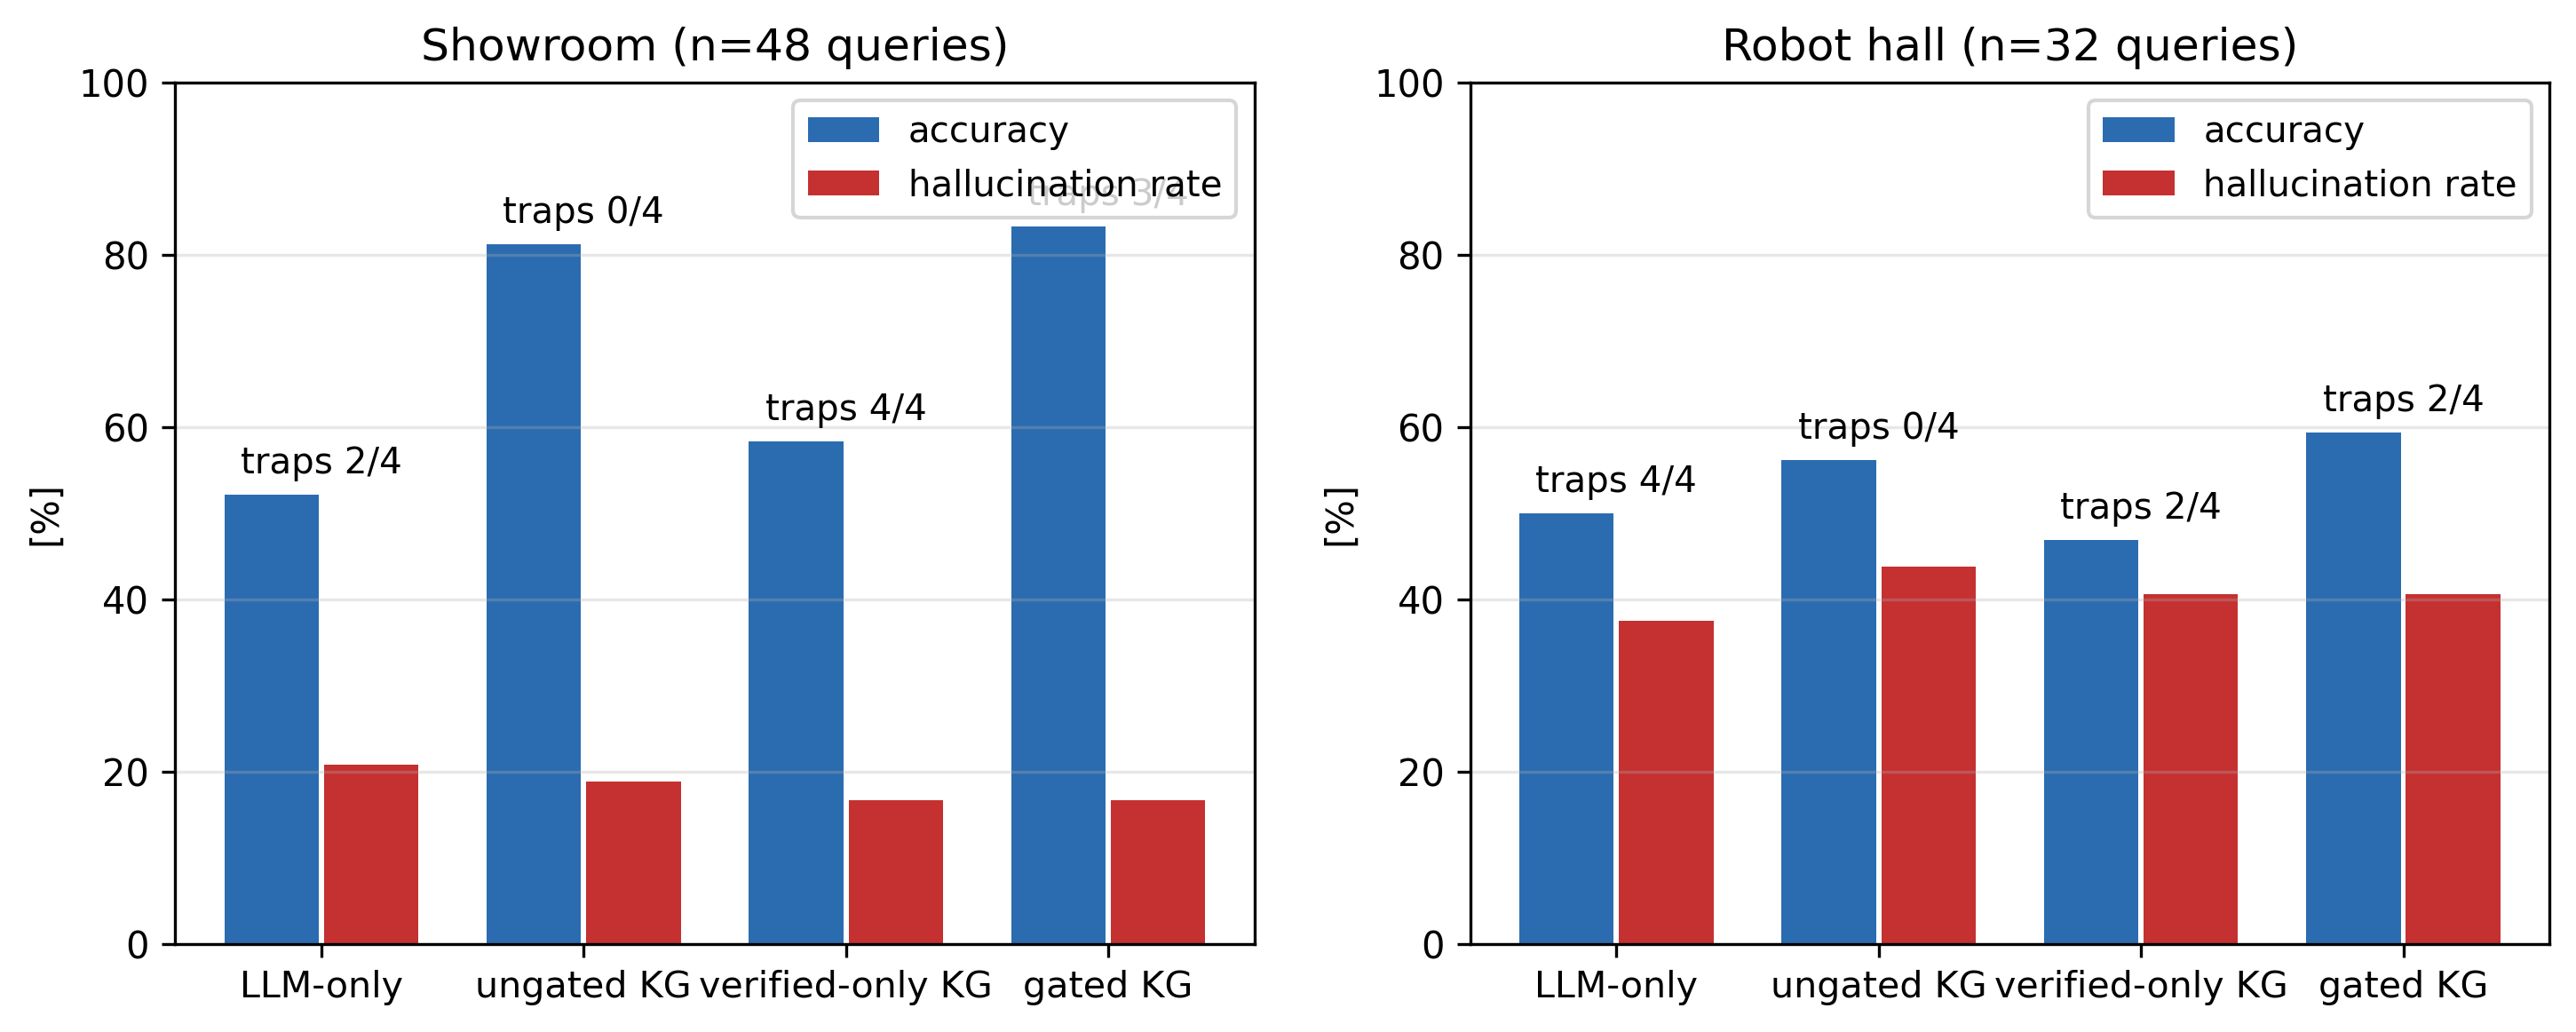
\includegraphics[width=0.9\linewidth]{figures/ele_fig7_query_benchmark.png}
\caption{Four-condition query benchmark with trap-question panel.}
\label{fig:query}
\end{figure}

\section{Incremental Update Evaluation}
\label{sec:exp-update}

\paragraph{Synthetic scenarios.}
Controlled edits of the room-scoped robot hall isolate matcher behavior
(Figure~\ref{fig:update}): (A)~unchanged repeat: 55/55 nodes carried, zero VLM
calls, zero identity switches; (B)~move: 1/1 moved with ID preserved;
(C)~remove+insert: exact absent/insert classification; (D)~occlusion: at 20\%
crop both affected objects still match, at 40\% matching fails into 2
false-absents + 2 false-news---the matcher's quantified breaking point. On the
combined-edit re-scan (move, insertion, and removal applied together),
selective re-verification re-ran Stage~B on only the two changed clusters: 26
of 822 VLM calls, \$0.23 versus \$7.37 for a full re-verification---3.1\% of
rebuild cost, and 0\% for scenario~A. The claim is scoped precisely: the 3.1\%
figure comes from a controlled same-quality re-scan where unchanged clusters
reproduce byte-identically; on the real T2$\rightarrow$T3 transition the scan
protocol itself changed, no cluster hash matched, and the epoch paid full
verification cost (\$3.54 for 41 clusters).

\begin{figure}[!htb]
\centering
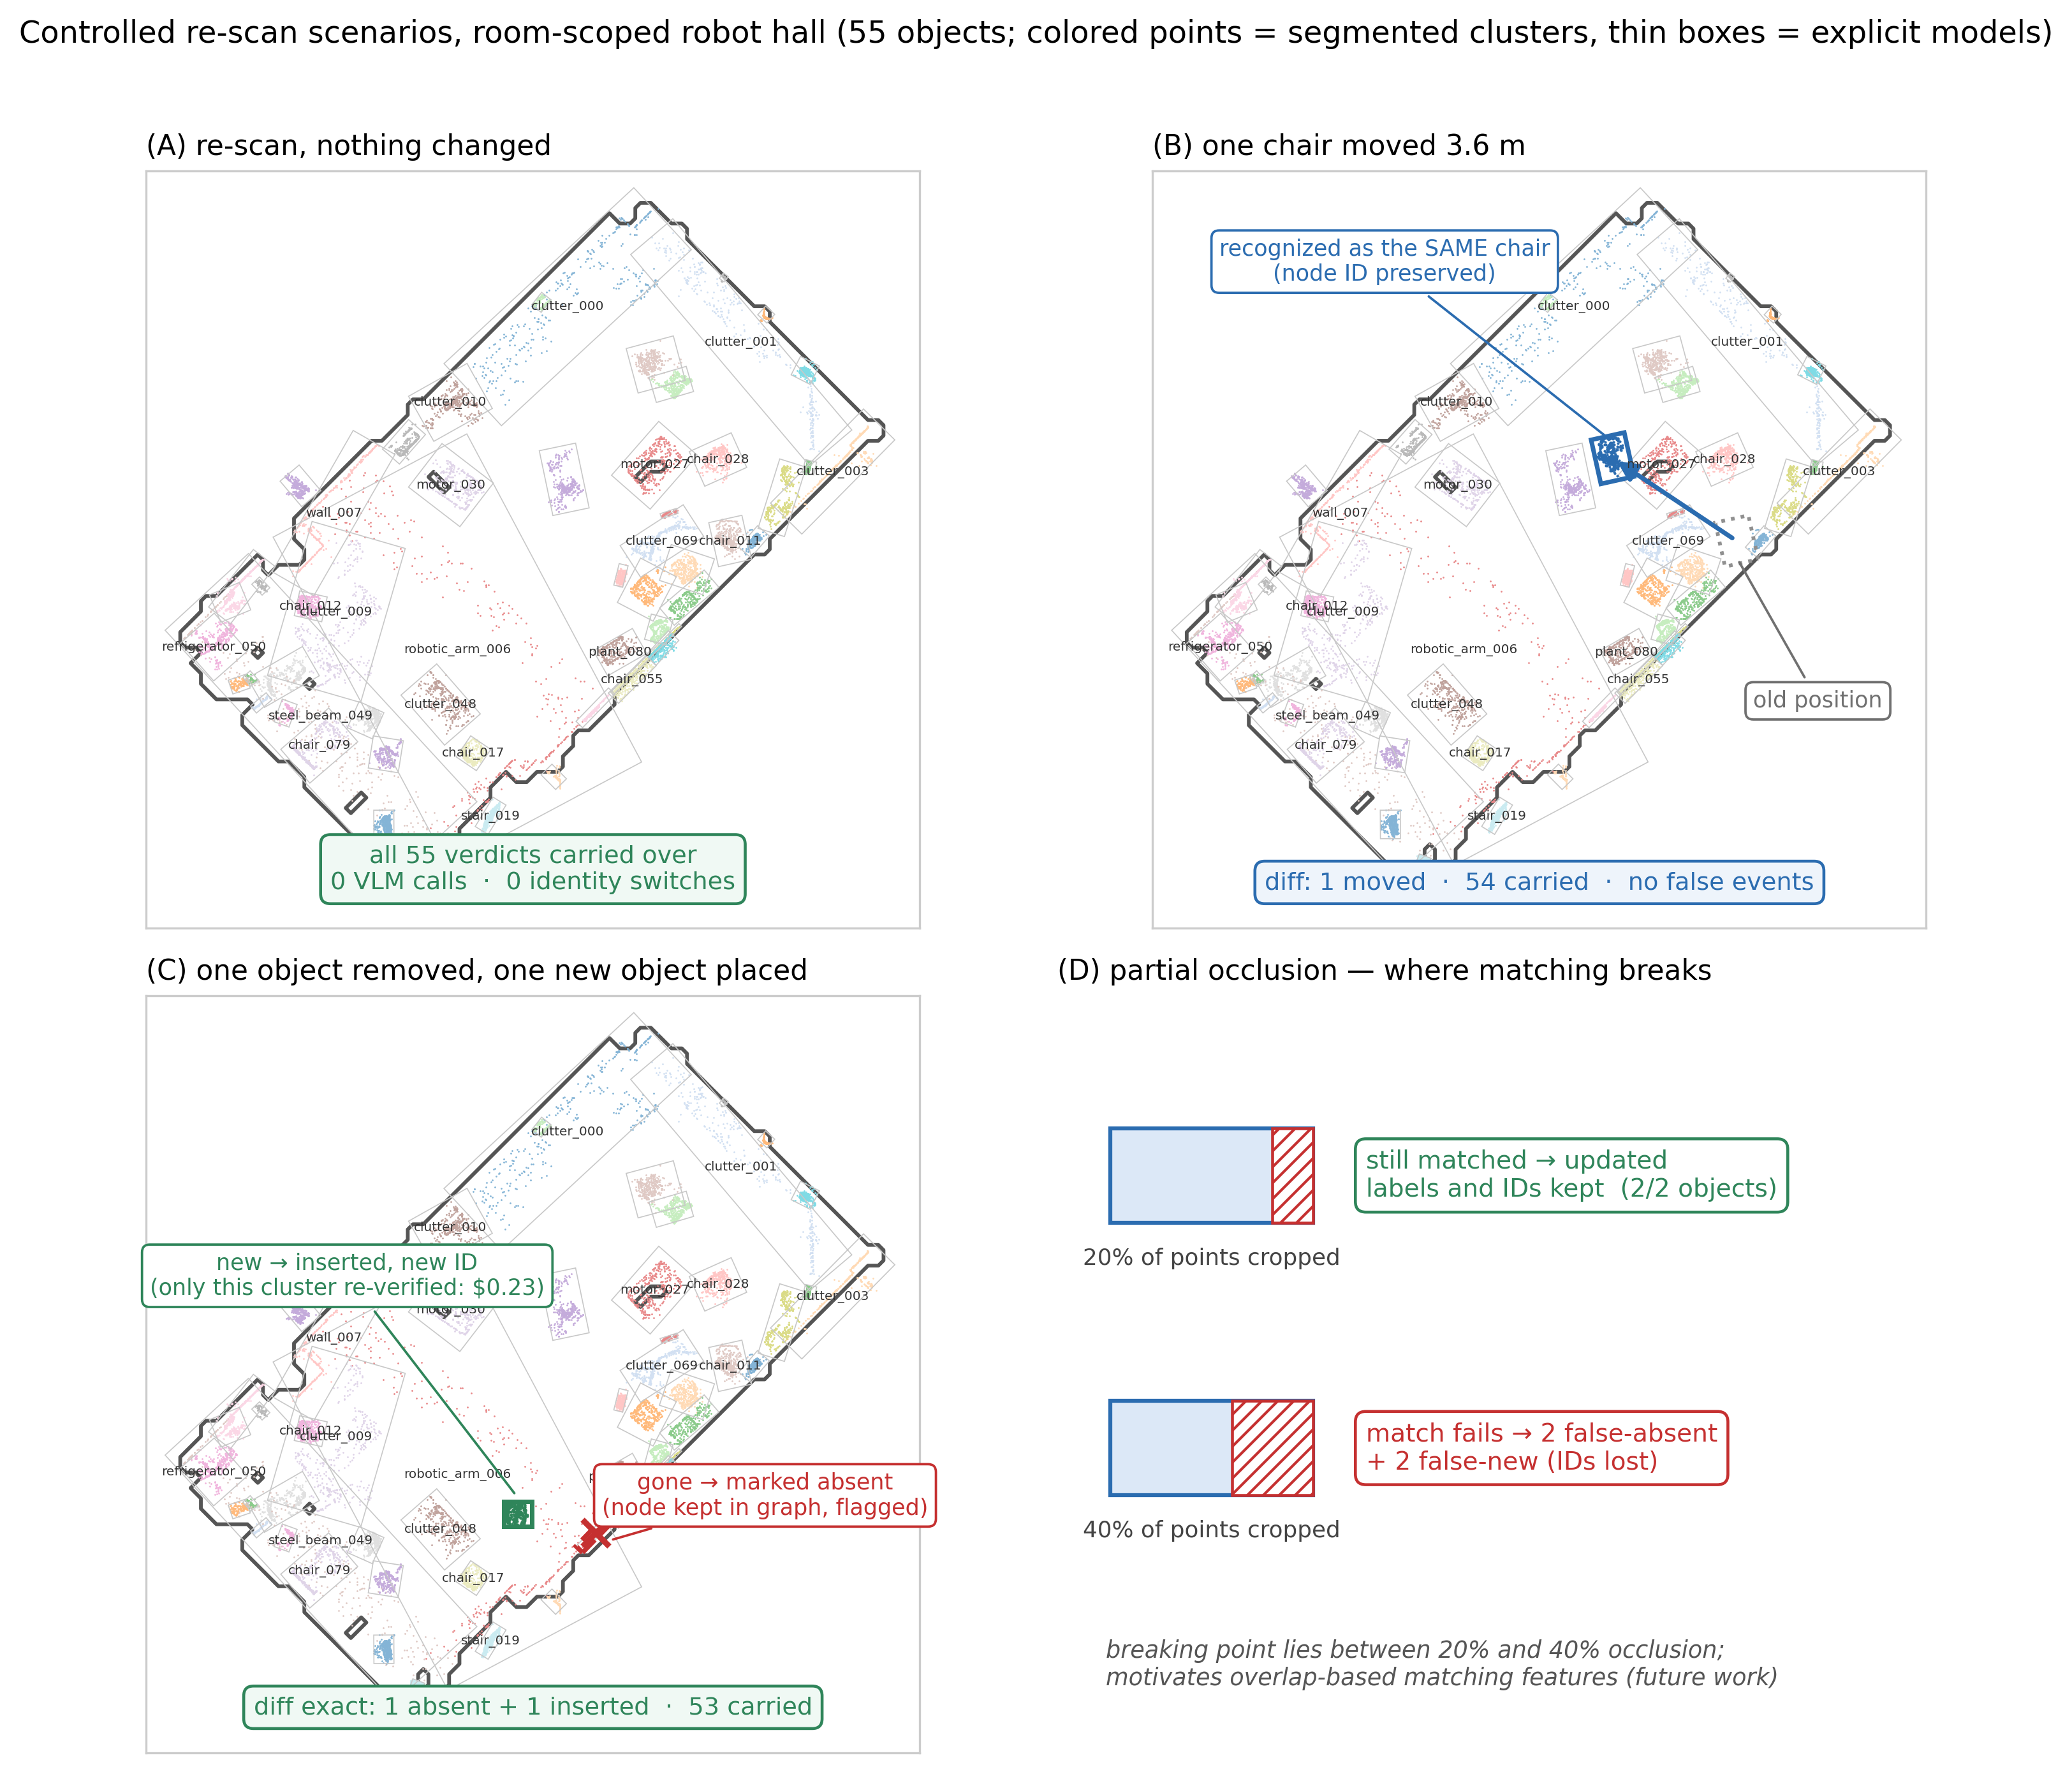
\includegraphics[width=0.9\linewidth]{figures/ele_fig8_incremental_update.png}
\caption{Controlled re-scan scenarios A--D (room-scoped robot hall, 55
objects), top-down view; each edited object is annotated with the matcher's
decision. (A)~A repeat scan carries all 55 verdicts at zero VLM cost. (B)~A
3.6~m chair move is classified \texttt{moved} with its node ID preserved.
(C)~A removed object is marked \texttt{absent} and a newly placed object is
\texttt{inserted}; only the insertion is re-verified. (D)~Partial occlusion:
both cropped objects still match at 20\%, but at 40\% matching fails.}
\label{fig:update}
\end{figure}

\paragraph{Real three-epoch study.}
The three epochs form a real update sequence: T1 (manual, June) $\rightarrow$
T2 (exploration, early July) $\rightarrow$ T3 (99.6\%-coverage exploration
with a controlled-change protocol, late July). Cross-epoch registration is
fully automatic (FPFH~\cite{rusu2009fpfh}+RANSAC then ICP~\cite{besl1992icp};
5.1~cm RMSE for T1$\rightarrow$T2, 4.2~cm for T3$\rightarrow$T2). The
T1$\rightarrow$T2 diff records the room's exhibition-to-test-hall
reorganization (updated 4 / moved 3 / inserted 48 / absent 31; among the moves,
a fire extinguisher displaced 3.0~m) and motivated the generic-type exclusion
in the move pass. The T2$\rightarrow$T3 diff (matched 9 / moved 1 / inserted 31
/ absent 45, Figure~\ref{fig:epochs}) sits on top of measured natural drift:
only 65\% of in-room object geometry is mutually supported at 10~cm between the
two scans, taken two weeks apart. To score the real transitions without circular
reference to the matcher, an independent correspondence reference was built by
bidirectional point overlap between epochs (4 strong and 6 partial static
pairs for T1$\rightarrow$T2, 7 strong and 5 partial for T2$\rightarrow$T3).
Matching accuracy on strong pairs is 2/4 and 4/7; \textbf{identity switches
are zero on both transitions}---every miss is a fragmentation error in which
re-segmentation changed an extent beyond the 30\% tolerance, so the object was
marked absent and re-inserted under a new ID, never associated with the wrong
object. Strict false-new and false-absent counts are 2/2 and 3/3, and all
three recorded \texttt{moved} claims are consistent with the reference (the
chair move is additionally owner-confirmed). Against the controlled-change
protocol, the system detected 2/2 physical changes at geometry level: the
moved chair is the epoch's only \texttt{moved} node (0.64~m, ID preserved
since T1), and the introduced floor fan was correctly \texttt{inserted} but
typed \texttt{clutter}. The fire extinguisher, pump, industrial robot, and
several chairs retain their minted IDs through both reorganizations, and the
place layer re-derives per-epoch names on the same regions (exhibition-era
\texttt{machine\_access\_area} $\rightarrow$ test-era
\texttt{machine\_operator\_station}) at about \$0.03 per epoch.

\begin{figure}[!htb]
\centering
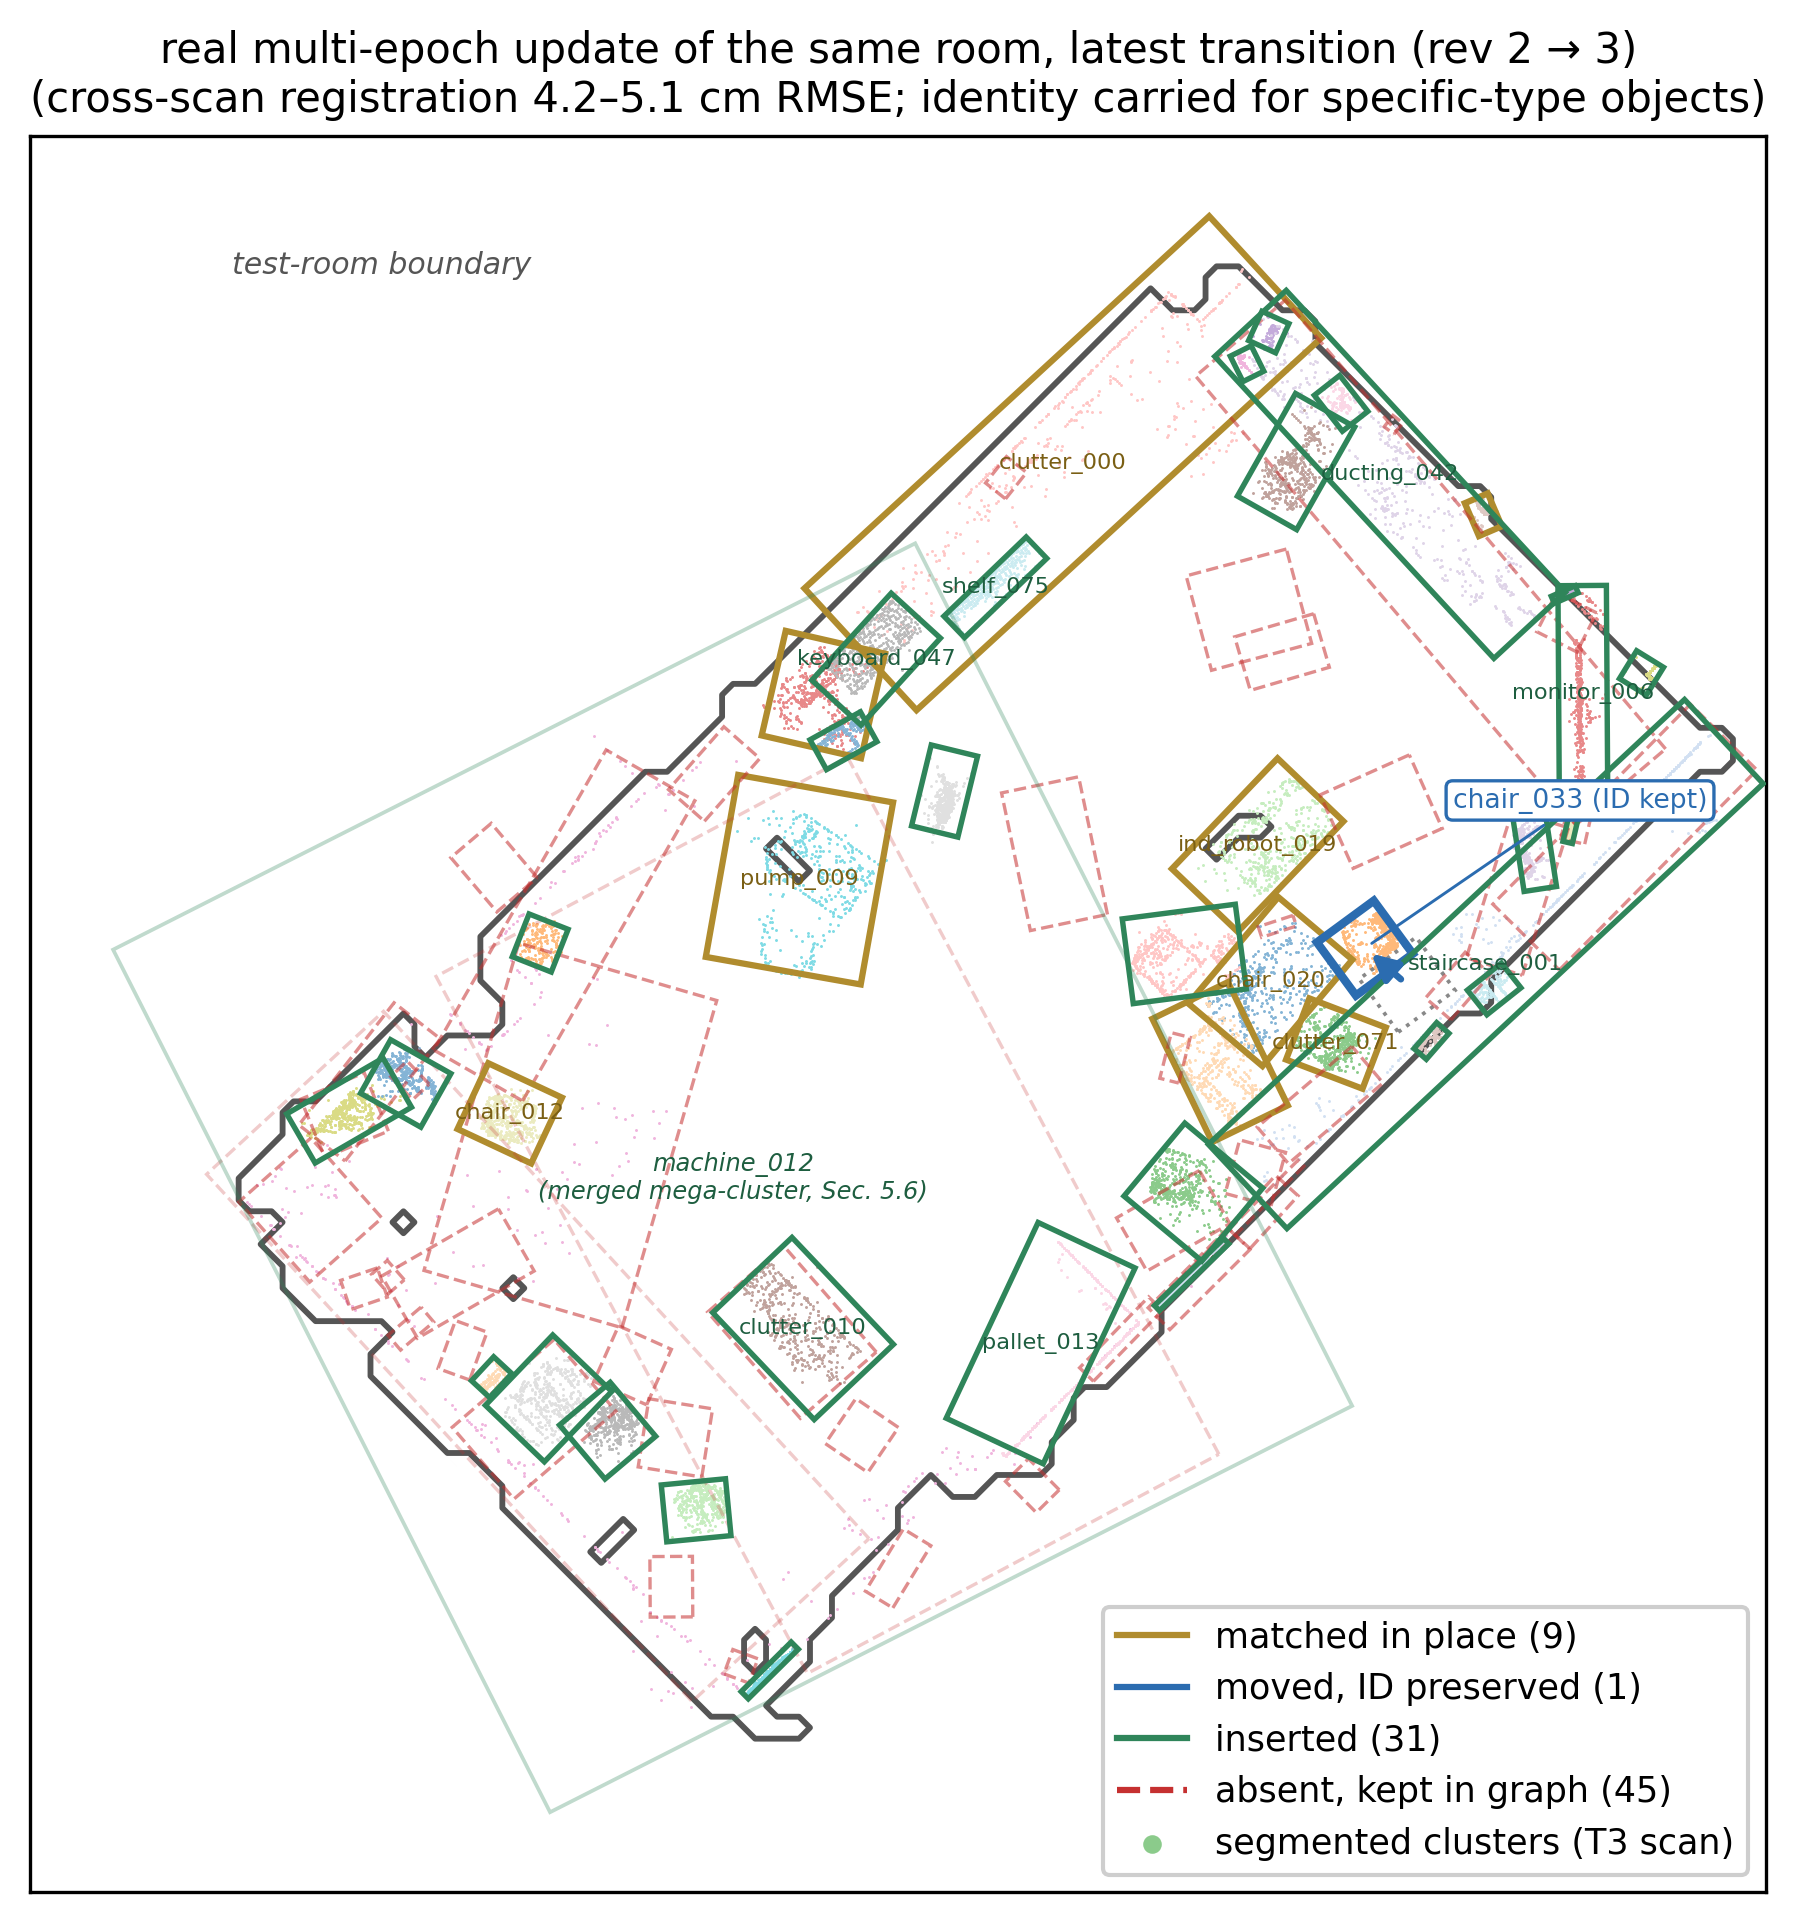
\includegraphics[width=0.9\linewidth]{figures/ele_fig9_two_epoch_update.png}
\caption{Real multi-epoch update, latest transition (T2$\rightarrow$T3),
top-down view: yaw-rotated node footprints colored by diff state (matched,
moved with ID preserved, inserted, absent). Oversized footprints of merged
mega-clusters are faded.}
\label{fig:epochs}
\end{figure}

\section{Retrospective End-to-End Replay}
\label{sec:exp-endtoend}

After the corrective machinery stabilized, the entire pipeline was re-run from
the raw T3 scan with no owner input at execution time and scored against the
live knowledge graph---by then a 46-object inventory embodying every owner
restoration, refutation, and correction. Because the corrective mechanisms were
developed from failures observed in this same environment, this is a
retrospective replay on the development scene, not an independent
generalization test: an independent \emph{run} on a non-independent
\emph{scene}. The cafeteria is the only scene independent in both senses, and
one corrective layer transfers mechanically to it: applying the hybrid
structure filter to the cafeteria with its T3 rules frozen flags both
ceiling-noise clusters with zero false positives, while the seven carpet
floor-noise clusters fall outside its rule families entirely.
Table~\ref{tab:layers} reports cumulative geometric recall as each automated
layer is enabled. The verified path alone recovers 28\%; diffuseness-gated
re-splitting nearly doubles it; the wall-compound gate (which self-triggers on
the monitor wall) and the structure-condition ensemble bring automated recall
to 85\%. Type accuracy saturates far lower ($\sim$31\% of recalled
objects)---the label bottleneck is the correlated verifier bias, and closing
it is precisely the owner layer's role. For calibration within the lineage's
own reporting style, DK-SMF reports 78--81\% detection accuracy against
predefined ground-truth objects in its RGB-D environments~\cite{joo2025dksmf};
the 85\% here is measured against an owner-audited inventory that includes
partially scanned and wall-flush objects, though the sensing modality and
ground-truth protocols differ. Each added layer admits more candidate
clusters, so automated recall is bought with review burden---exactly the
owner-review efficiency the model should optimize.

\begin{table}[htbp]
\centering
\caption{Cumulative automated recall of the full re-run against the
owner-corrected 46-object graph (no owner input in the run itself).}
\label{tab:layers}
\begin{tabular}{l c c}
\toprule
\textbf{Automated layers (cumulative)} & \textbf{GT recall} & \textbf{In-room precision} \\
\midrule
Verified path (backbone + verification) & 13/46 (28\%) & 37\% \\
+ diffuseness re-split & 26/46 (57\%) & 53\% \\
+ wall-compound gate & 36/46 (78\%) & 60\% \\
+ structure-condition ensemble & 37/46 (80\%) & 49\% \\
+ wall-compound panel square-up & \textbf{39/46 (85\%)} & 51\% \\
\bottomrule
\end{tabular}
\end{table}

\section{Ablation, Verifier Comparison, and Cross-Floor Stress Scene}
\label{sec:exp-ablation}

\paragraph{Gating style, pose context, and vocabulary.}
Instructing the model to respect verification status blocks 1/4 traps;
structural demotion blocks 4/4 under identical prompts in this isolated
comparison (versus 3/4 end to end)---the single strongest argument that
reliability must live in the data contract, not in instructions. Injecting
mounting-height context removed all three phantom ceiling keyboards in its
pilot, but applying it to every object \emph{reduced} escalated accuracy
($88.9\%\rightarrow75.0\%$), so it is deployed only as a targeted defense
and, later, as the coarse height-level attribute. Swapping the
Stage-A classifier vocabulary ranks generic-30 (66.7\%) above curated-20
(48.7\%) and above the owner-derived 18-term set (33.3\%): narrowing the prompt
set toward the deployment vocabulary \emph{hurts} the embedding-level
classifier, confirming the domain gap that motivates VLM verification.
Removing the provisional label from the verifier's context collapses
decisiveness (trigger rate $58\%\rightarrow90\%$, unanimity
$21\rightarrow5$ objects) and lowers escalated accuracy to 38.9\%: Stage~B is a
verifier of hypotheses, and the provisional label is load-bearing context,
which is why label adoption is agreement-gated and owner-auditable rather than
trusted outright.

\paragraph{Verifier model.}
Running the identical Stage-B protocol across five commercial verifiers (two
vendors, three tiers, two generations) makes escalation an economic instrument
(Table~\ref{tab:vlmcmp}): call volume tracks verifier decisiveness
monotonically (247 to 383 calls as unanimous verifications fall from 26 to 9).
Within a generation, the smaller tier splits more votes and resolves fewer,
inflating call volume by 14\% and eroding part of its nominal per-token
price advantage; all three current-generation frontier models tie on type
accuracy against the owner inventory (7/13) but differ twofold in the escalations
they need (9 versus 18); and the ranking is generation-dominated, not vendor-dominated.
Escalation volume is thus a label-free, online proxy for verifier decisiveness
on the deployment's own data---a practical criterion for verifier selection
under cost constraints---but not a proxy for accuracy: re-running both main
scenes under the most decisive model lowers escalation triggers (58\%
$\rightarrow$ 50\%, 51\% $\rightarrow$ 33\%) but also unanimous precision
(100\% $\rightarrow$ 91.7\%, 94.4\% $\rightarrow$ 83.3\%), re-distributing error
mass from indecision into confident under-labeling. Verifier upgrades change
\emph{where} errors live rather than uniformly removing them, which is why the
framework treats verification as tiered evidence behind a gate: the tier
structure, the escalation economics, and the owner loop survive a verifier
swap; the specific precision figures do not.

\begin{table}[htbp]
\centering
\caption{Verifier-model comparison: identical Stage-B late fusion +
escalation on the same 35 in-room T3 clusters, scored against the
owner-corrected graph. Type-correct = canonical-synonym match on the clusters
that geometrically match a ground-truth object; cost at vendor list rates of
August 2026.}
\label{tab:vlmcmp}
\footnotesize\setstretch{1.15}
\begin{tabular}{l c c c c c c}
\toprule
\textbf{Verifier} & Verified & Esc.-resolved & Unverified & Type-correct & Calls & Cost \\
\midrule
Claude Sonnet 5 & \textbf{26} & 3 & \textbf{6} & \textbf{7/13} & \textbf{247} & \$2.49 \\
GPT-5.6 & 21 & 7 & 7 & \textbf{7/13} & 287 & \$0.11 \\
Claude Opus 5 & 17 & 8 & 10 & \textbf{7/13} & 319 & \$5.28 \\
Claude Sonnet 4.6 & 15 & 6 & 14 & 6/13 & 335 & \$3.00 \\
Claude Haiku 4.5 & 9 & 9 & 17 & 5/13 & 383 & \$1.13 \\
\bottomrule
\end{tabular}
\end{table}

\paragraph{Cross-floor stress scene.}
The cafeteria scene probes the same protocol on a furnishing domain the
campaign never saw: carpeted floor, fabric sofa booths, planter partitions
(Figure~\ref{fig:cafe}). The backbone transfers mechanically---57~M points to
28 clusters in 13.5~s after an automatic wall-normal yaw alignment---but
verification does not (Table~\ref{tab:cafe}): escalated accuracy reaches only
35\% against confirmed owner ground truth, and unanimous precision falls to
57.1\%, with two unanimous keyboard phantoms on carpet-noise clusters. The
errors are structured: the scene's dominant object family---the sofas---enters
the pipeline pre-broken, split into five cushion fragments and two sofa--table
merges, and every one is absorbed; carpet pile leaves seven residual
floor-noise clusters above the RANSAC floor plane, the floor-material analogue
of the ceiling remnants; and the confidence gate quarantines 9 of the 16 wrong
labels as unverified while the unanimous errors pass. Two upgrades applied
factorially act on different error classes: re-rendering the identical view
sets from full-resolution points repairs \emph{whole-object} ambiguity (the
keyboard phantoms vanish, both chairs and both doors recover), and the
verifier upgrade adds accuracy on top of whichever source it is given
($35\rightarrow45\%$ on voxel, $40\rightarrow60\%$ on full-resolution sets).
Symmetric controls that re-render both industrial scenes from full-resolution
points \emph{reverse} the effect (showroom escalated accuracy
$88.9\rightarrow80.6\%$; robot hall $84.4\rightarrow68.8\%$), because added
texture invites over-specific labels; the main campaign's voxel-source
protocol therefore stands as the right default for the industrial scenes.
What neither lever reaches is fragmentation: the seven sofa clusters are
absorbed in all four cells. Segmentation bounds what any verifier can see;
render quality bounds what a given verifier resolves; the model generation
buys accuracy only on top of both. Tier precision is therefore a scene- and
domain-scoped measurement, to be re-estimated per deployment via a small
owner-confirmed probe set, rather than a property of the architecture.

\begin{table}[htbp]
\centering
\caption{Cafeteria stress scene: verification under verifier $\times$ render
source (identical 512-px multi-view protocol). Accuracy is escalated accuracy
on confirmed GT ($n=20$; the fragment-excluded column drops the five confirmed
sofa-fragment clusters, $n=15$). In every cell, 0 of the 7 sofa clusters are
recovered.}
\label{tab:cafe}
\begin{tabular}{l l c c c c}
\toprule
\textbf{Verifier} & \textbf{Render source} & Esc.\ acc. & (excl.\ fragments) & Unan.\ prec. & Trigger \\
\midrule
Sonnet 4.6 & 3~cm voxel cloud & 35.0\% & 46.7\% & 57.1\% & 68\% \\
Sonnet 4.6 & full-resolution & 40.0\% & 53.3\% & 62.5\% & 60\% \\
Sonnet 5 & 3~cm voxel cloud & 45.0\% & 60.0\% & 66.7\% & 40\% \\
Sonnet 5 & full-resolution & \textbf{60.0\%} & \textbf{80.0\%} & \textbf{80.0\%} & 52\% \\
\bottomrule
\end{tabular}
\end{table}

\begin{figure}[!htb]
\centering
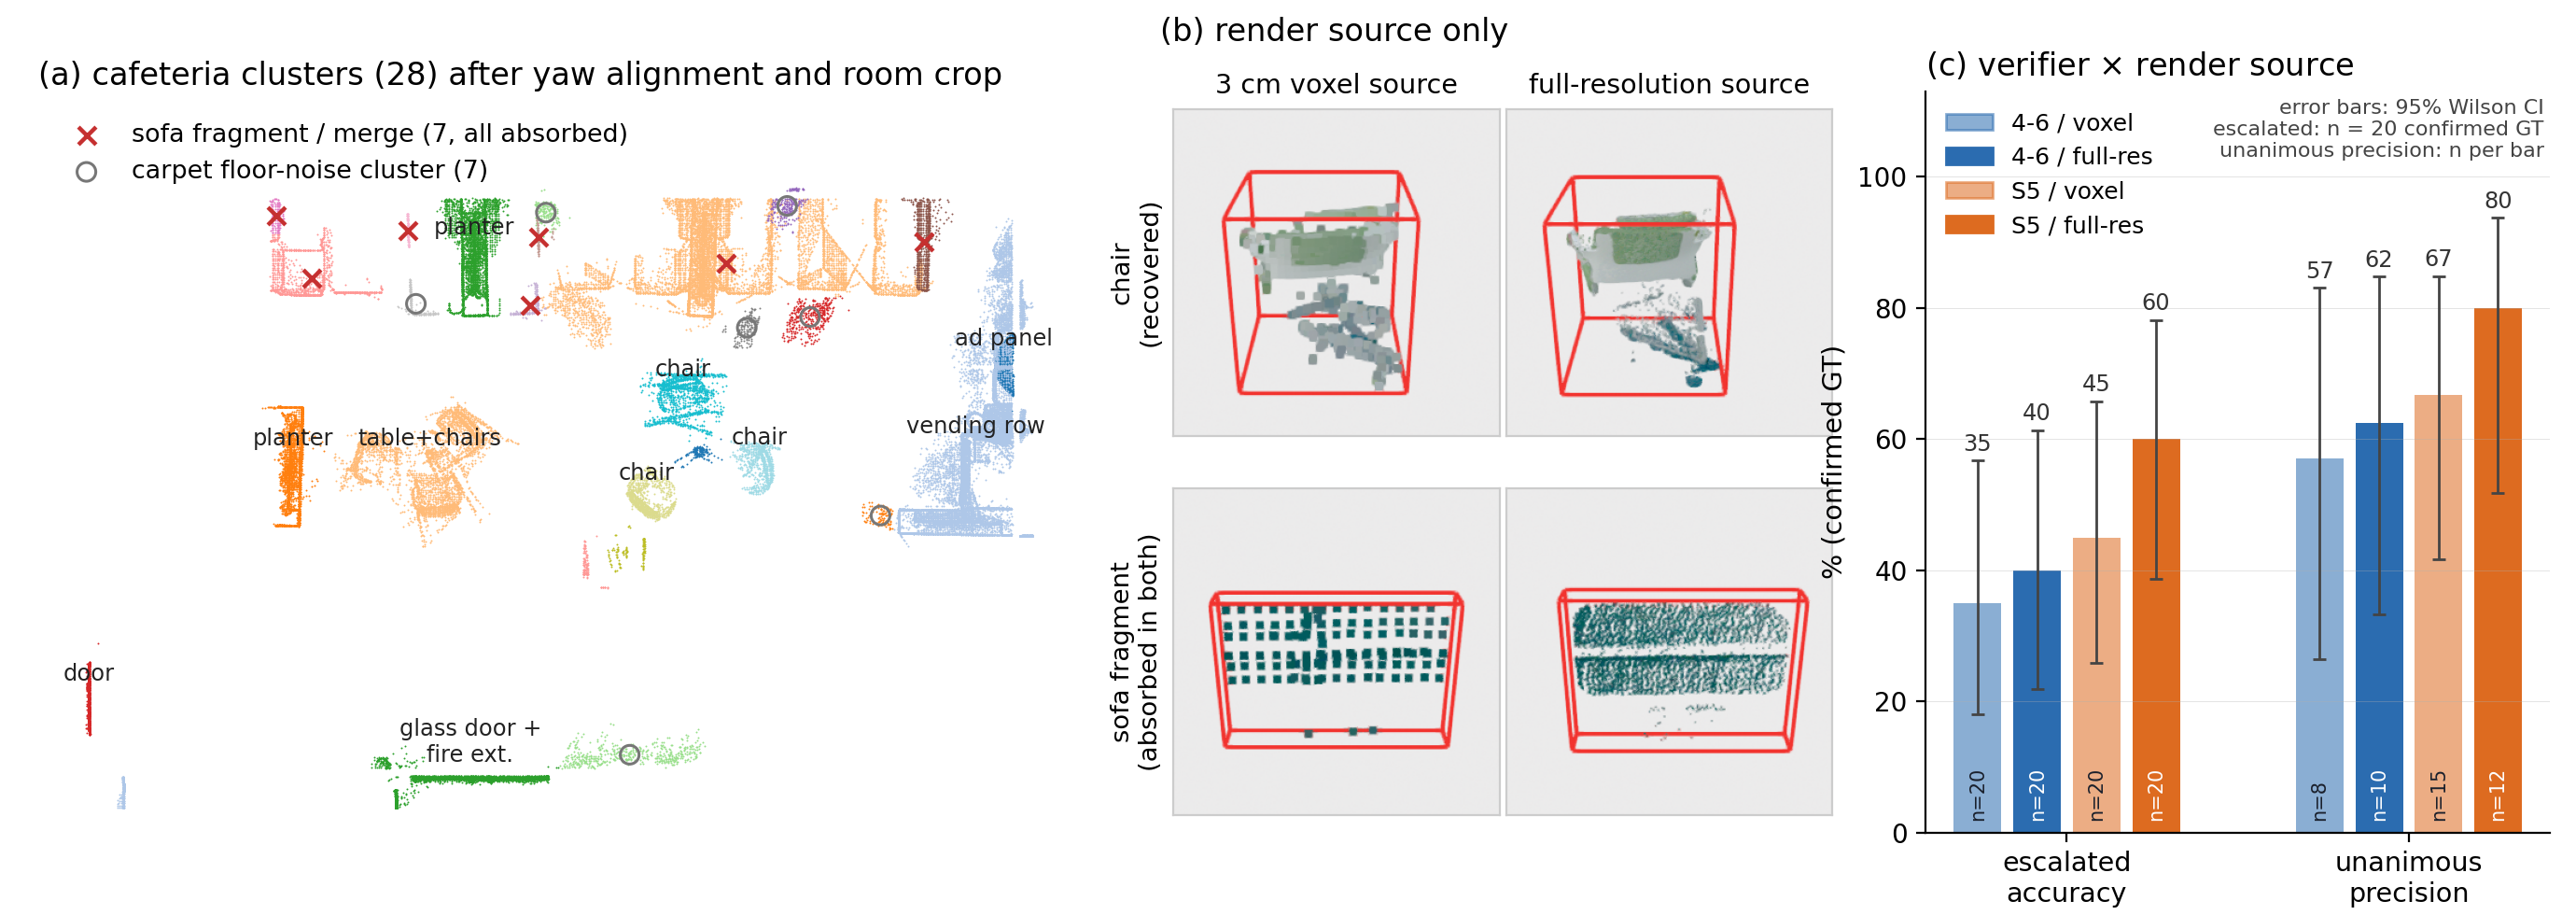
\includegraphics[width=\linewidth]{figures/ele_fig17_cafe_stress.png}
\caption{Cafeteria stress scene. (a)~The 28 clusters after automatic yaw
alignment and room crop; crosses mark the seven sofa fragments/merges,
circles the seven carpet floor-noise clusters. (b)~One cluster rendered from
the 3~cm working cloud (left) and from full-resolution re-associated points
(right): the chair (top) is recovered by the render-source change alone; the
sofa fragment (bottom) is not. (c)~Escalated accuracy and unanimous precision
across verifier $\times$ render source; error bars are 95\% Wilson intervals.}
\label{fig:cafe}
\end{figure}

\paragraph{Cost and latency.}
VLM verification is the only paid stage: full verification averages
$\sim$\$0.09 per object (\$3.63 for a 38-cluster run and \$7.37 for the
86-cluster robot-hall detection set, all calls included), and the incremental
design changes the cost model qualitatively (an identical-input repeat scan
costs \$0). Wall-clock time is equally bounded on the workstation: the full
deterministic backbone---loading the 68.6~M-point E57, 3~cm downsampling,
ten-plane removal, decomposition, and remnant filtering---completes in 29~s
(8.1~GB peak memory), rendering the four-view sets takes 99~s for 88 objects,
and verification with escalation runs in 7.7~min for a 50-object scene at six
concurrent calls, so the complete semantic modeling of a scene finishes in
well under ten minutes end to end. Verification is offline; no VLM call sits
on a robot's control path. Figure~\ref{fig:semmap} visualizes the resulting
semantic map with the confidence gate visible in the map itself.

\begin{figure}[!htb]
\centering
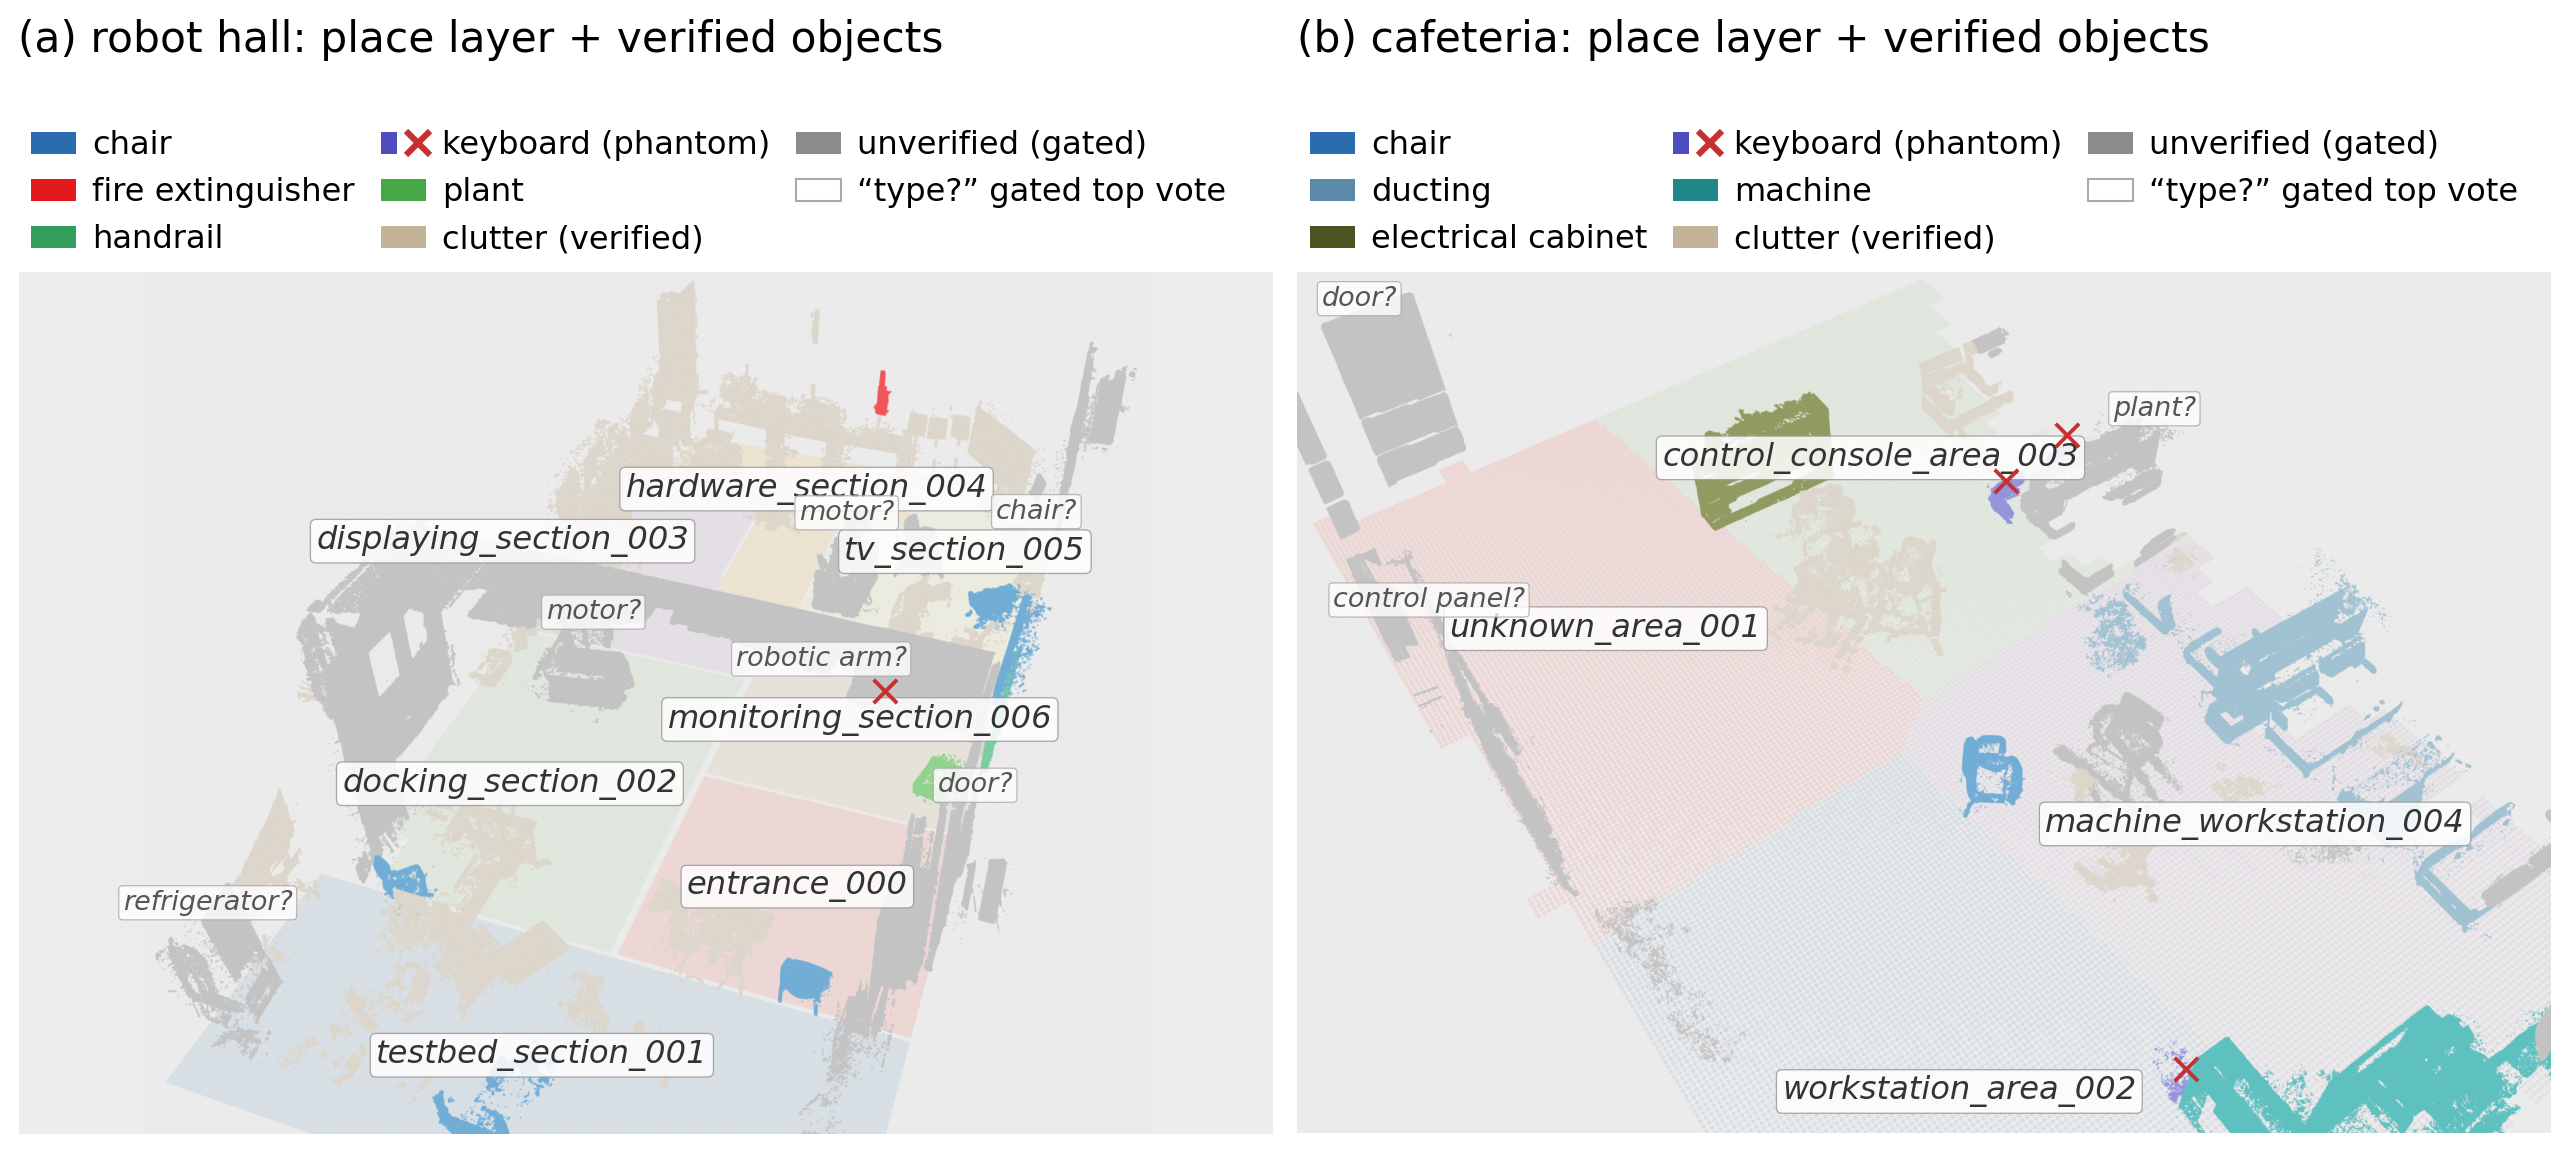
\includegraphics[width=\linewidth]{figures/ele_fig19_semantic_map.png}
\caption{The generated semantic map, visualized at the verification stage
(before owner feedback), so the confidence gate and the errors that pass it
are both visible. (a)~Robot hall: SLIC place-layer regions (pastel floor) with
the room-scoped object clusters rendered as their segmented points, colored by
verified class; gray clusters are \texttt{unverified} and demoted at query
time. (b)~The cafeteria stress scene under the same representation; red
crosses mark verified-keyboard clusters that are owner-refuted phantoms.}
\label{fig:semmap}
\end{figure}

\section{Digital Twin: Conversion, Performance, and Fidelity}
\label{sec:exp-twin}

All twin experiments ran on the desktop workstation of
Section~\ref{subsec:platforms} (Isaac Sim~5.1, ROS~2 Jazzy).

\paragraph{Conversion time and resources.}
Table~\ref{tab:convtime} reports single-run wall-clock times for each pipeline
stage on the 68.5~M-point scan. The complete conversion from raw E57 to a
simulation-ready USD stage takes 78.5~s; the dominant cost is writing the
3.7~M-point visual layer, and a reduced-density variant (485~K points)
completes in 36.5~s. The conversion runs entirely on the CPU, peaking at 8.1~GB
of resident memory with an average utilization of 2.4 cores; the simulator
process occupies 3.1~GB of GPU memory with the full scene and robot
articulation loaded in headless physics-only mode. Authoring a comparable
environment by hand is a multi-day effort, and, unlike manual modeling, the
pipeline can be rerun after every facility change. Every stage is linear in
the number of input points, so conversion time scales roughly linearly with
scan size; the main memory constraint is holding the merged cloud in RAM,
which for facility-scale scans beyond roughly $10^8$ points would call for
chunked streaming of the E57 input.

\begin{table}[htbp]
\centering
\caption{Scan-to-simulation conversion time (68.5~M-point E57). Source:
RAAICON~2026~\cite{raaicon2026}.}
\label{tab:convtime}
\begin{tabular}{l r}
\toprule
\textbf{Stage} & \textbf{Time (s)} \\
\midrule
Floor RANSAC, occupancy grid, ROS map export & 14.8 \\
Dense visual cloud extraction (voxel 0.015~m) & 16.8 \\
Visual layer USD export (3.7~M points) & 46.8 \\
Collision-layer synthesis (1{,}430 boxes) & 0.1 \\
\midrule
\textbf{Total} & \textbf{78.5} \\
\bottomrule
\end{tabular}
\end{table}

\paragraph{Scene complexity and simulation performance.}
The generated stage contains 1{,}430 collision boxes ($\approx$17~K
triangles) and 3{,}725{,}047 rendered points (166~MB USD). With the AMMR
articulation loaded (physics at 120~Hz), headless physics-only simulation
advances at 675 steps/s, a real-time factor of 5.6; with rendering enabled the
simulator sustains 51 rendered frames per second (real-time factor 0.84), and
in the interactive GUI session used for the on-site experiments the viewport
sustained 104 frames per second with the full point layer in view. Before
coupling to the real robot, the swerve base was validated in simulation:
straight-line (1.13~m forward run), lateral (1.45~m strafe), and in-place
rotation ($65^{\circ}$) maneuvers each produced odometry matching the
commanded motion direction, and the flip hysteresis of
Equation~\ref{eq:swerve} eliminated the wheel-speed oscillation otherwise
observed at steering-wrap boundaries.

\paragraph{Live twin verification and simulator-issued goals.}
The bridge contract was verified end to end with the physical AMMR in the
scanned facility (Figure~\ref{fig:pairroom}): the 30~Hz state stream is
received across the Wi-Fi link, the anchor calibration of
Equation~\ref{eq:anchor} converges from a single pose sample, and goals picked
in the simulator drive the real robot through Nav2. During the on-site session
the twin mirrored teleoperated motion continuously across a 3.4~m sweep of the
room. Across two sessions on consecutive days, all four navigation goals
issued by dragging the target marker in the simulator viewport drove the robot
to the corresponding physical locations (Table~\ref{tab:goaltrials},
Figure~\ref{fig:pairgoal}); the twin-frame arrival error of 0.19--0.23~m
(mean 0.21~m) is consistent with the Nav2 goal tolerance, at commanded speeds
up to 0.52~m/s.

\begin{table}[htbp]
\centering
\caption{Simulator-issued navigation-goal trials on the physical AMMR.
Source: RAAICON~2026~\cite{raaicon2026}.}
\label{tab:goaltrials}
\begin{tabular}{c c c l}
\toprule
\textbf{Trial} & \textbf{Session} & \textbf{Error (m)} & \textbf{Note} \\
\midrule
1 & day 1 & 0.19 & 14.4~s run \\
2 & day 1 & 0.21 & \\
3 & day 2 & 0.19 & \\
4 & day 2 & 0.23 & 3.0~m straight, up to 0.52~m/s \\
\midrule
\multicolumn{2}{l}{\textbf{Mean (4/4 reached)}} & \textbf{0.21} & \\
\bottomrule
\end{tabular}
\end{table}

\begin{figure}[!htb]
\centering
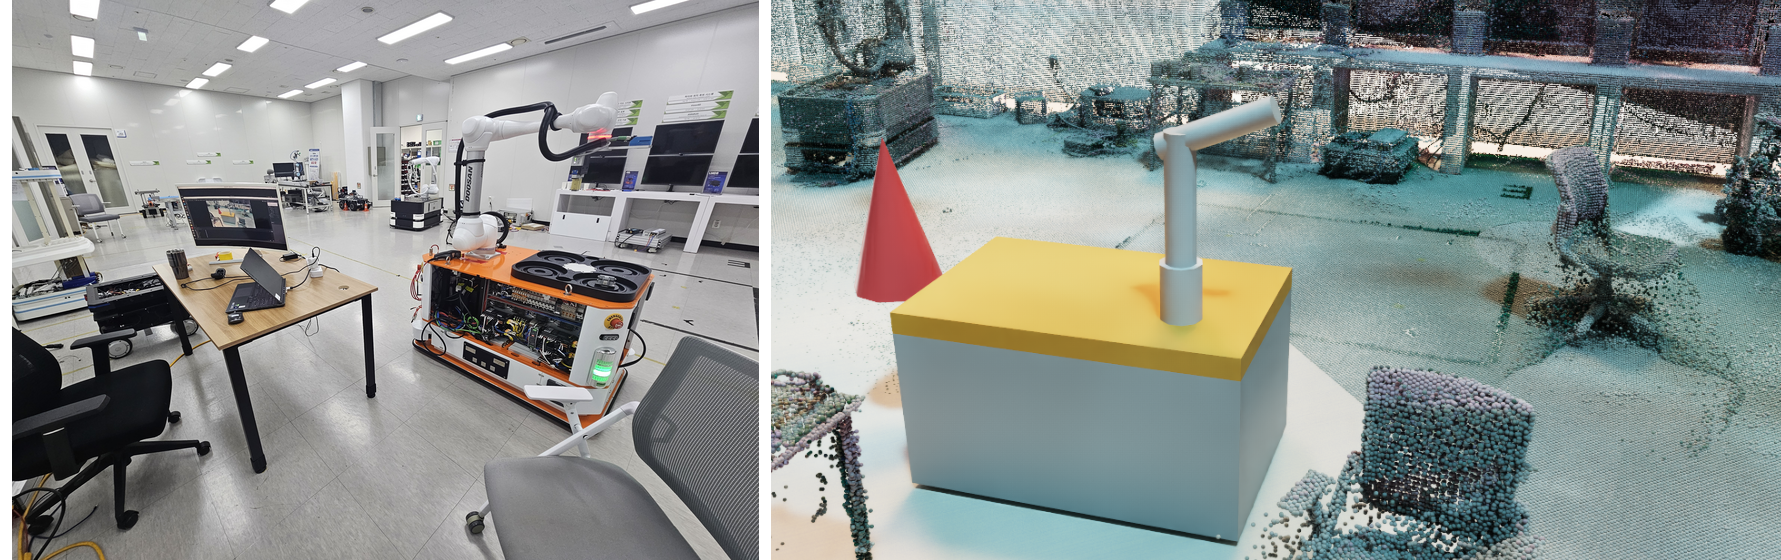
\includegraphics[width=0.95\linewidth]{figures/raa_fig_pair_room.png}
\caption{Test facility (left) and its generated twin during the live session
(right). The yellow body with the white column is the AMMR proxy model; the
red cone is the draggable navigation-goal marker.}
\label{fig:pairroom}
\end{figure}

\begin{figure}[!htb]
\centering
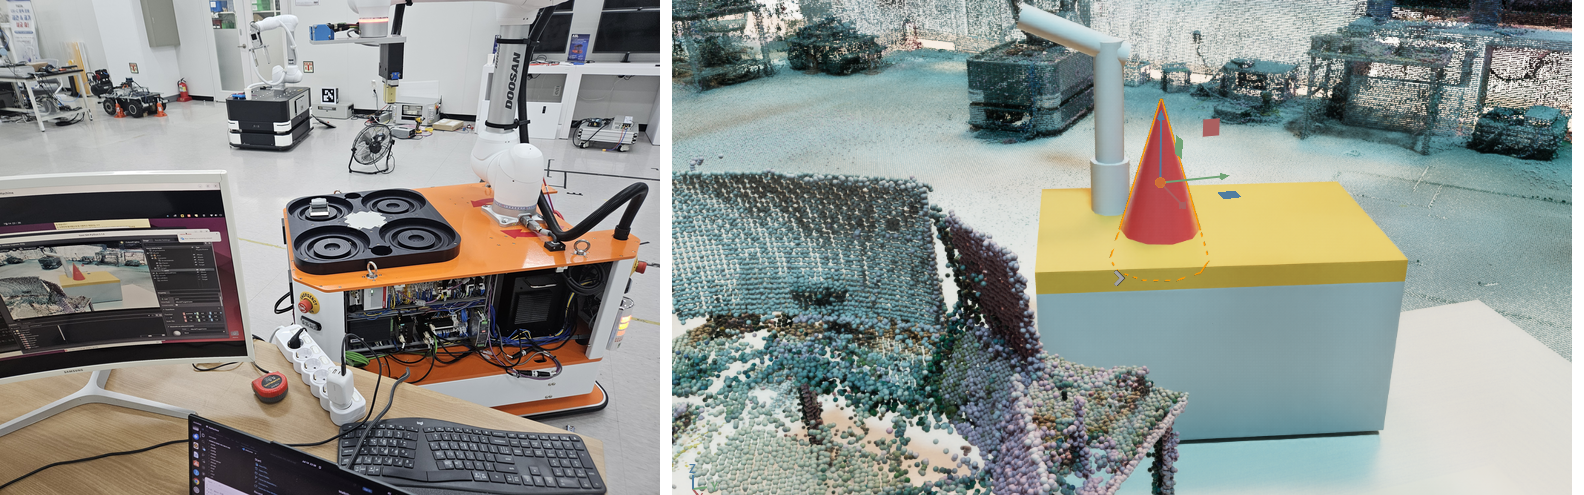
\includegraphics[width=0.95\linewidth]{figures/raa_fig_pair_goal.png}
\caption{Simulator-issued navigation goal. Left: the physical robot at the
reached location; right: the twin after arrival, parked on the goal marker.}
\label{fig:pairgoal}
\end{figure}

\paragraph{Geometric fidelity.}
Metric accuracy is evaluated at two levels. Three room features were
tape-measured and compared against the same dimensions extracted from the
twin's point layer (Table~\ref{tab:geo}): all errors are within 2\% (mean
absolute error 6.4~cm, or 1.3\%), so the scan-to-simulation conversion itself
preserves metric scale to centimeter level. End to end, tape-measured
distances between marked floor checkpoints were compared against the
corresponding distances reported by the twin with the robot parked on each
checkpoint, which captures the full error budget---TLS registration, occupancy
quantization, AMCL localization, and anchor calibration---without requiring a
global frame alignment. Over three checkpoint pairs (0.86, 3.14, and 1.30~m
tape distance) the twin distances deviated by a mean absolute error of 5.5~cm
(RMSE 7.4~cm, maximum 12.5~cm, signed bias $+2.8$~cm; Figure~\ref{fig:eval}).
The largest deviation occurred on the segment executed with large in-place
rotations and matches the AMCL repeatability observed when revisiting the same
floor marker (17~cm), indicating that end-to-end twin accuracy is dominated by
the onboard localization rather than by the reconstructed scene.

\begin{table}[htbp]
\centering
\caption{Scene-feature dimensions: tape measure vs.\ twin point layer.}
\label{tab:geo}
\begin{tabular}{l r r r}
\toprule
\textbf{Feature} & \textbf{Real (m)} & \textbf{Twin (m)} & \textbf{Error} \\
\midrule
Window-side wall length & 8.000 & 7.918 & $-1.0$\% \\
Double-door width & 1.700 & 1.680 & $-1.2$\% \\
Workbench row length & 5.010 & 5.100 & $+1.8$\% \\
\bottomrule
\end{tabular}
\end{table}

\begin{figure}[!htb]
\centering
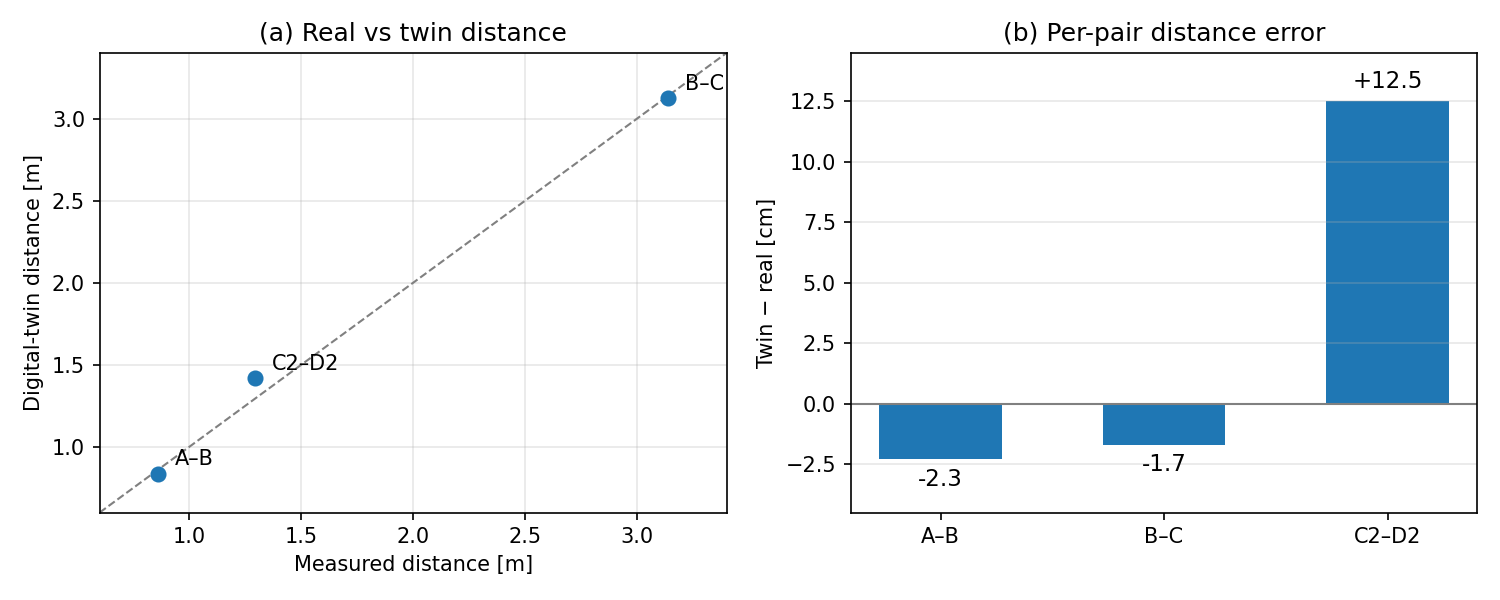
\includegraphics[width=0.95\linewidth]{figures/raa_fig_eval.png}
\caption{Checkpoint-pair distances, tape measure vs.\ twin: scatter against
the identity line (left) and signed per-pair error (right).}
\label{fig:eval}
\end{figure}

\section{Semantic Mission Execution in Simulation and on the Physical Robot}
\label{sec:exp-missions}

\paragraph{Simulation.}
In the Gazebo twin of the test room, over three repetitions of a
three-mission battery (approach the TV, go to the seating area, return home),
task success is 9/9, with mean leg path lengths 4.6/5.4/1.8~m and completion
times 16.5/24.9/15.0~s; semantic resolution latency (command to accepted or
refused goal) is under one second, and a gate refusal stops the robot safely
with zero motion. The reactive layer supplies the safety-stop behavior: a
low-battery event during navigation preempts the active Nav2 goal and returns
the platform to a holding position at home. The phantom experiment
(Table~\ref{tab:semnav}) sends the robot to three owner-refuted phantoms under
two knowledge states. Against the pre-feedback graph, all three phantoms carry
\emph{verified} labels, so the confidence gate passes them---and the waste
takes three distinct forms: a pointless drive to a fluorescent lamp; a
\emph{false arrival} at a 7.4~m ``staircase'' whose approach ring encloses the
robot's own position; and 22~s of futile replanning toward a wall-pillar
``book'' whose approach pose the platform's footprint cannot reach. Against the
graph after structure filtering and owner feedback, the same commands are
refused in about one second with zero motion (Figure~\ref{fig:semnav}).
Verification gating alone cannot stop verified phantoms; it is the combination
of gating, structure-noise removal, and owner feedback that reduces the robot's
exposure to phantom semantic claims.

\begin{table}[htbp]
\caption{Phantom-goal mission waste in simulation (AMMR proxy). The same three
commands are resolved against the knowledge graph before and after structure
filtering + owner feedback (both with the verification gate active).}
\label{tab:semnav}
\centering
\begin{tabular}{l l c c c}
\toprule
\textbf{KG state} & \textbf{Phantom target (truth)} & \textbf{Outcome} & \textbf{Wasted path} & \textbf{Wasted time} \\
\midrule
pre-feedback & keyboard (fluorescent lamp) & driven & 1.7~m & 16.8~s \\
pre-feedback & staircase (bare wall) & false arrival & 0.6~m & 5.7~s \\
pre-feedback & book (wall pillar) & unreachable, aborted & 0~m & 22.2~s \\
\midrule
filtered + owner feedback & all three & refused & 0~m & $\sim$1~s \\
\bottomrule
\end{tabular}
\end{table}

\begin{figure}[!htb]
\centering
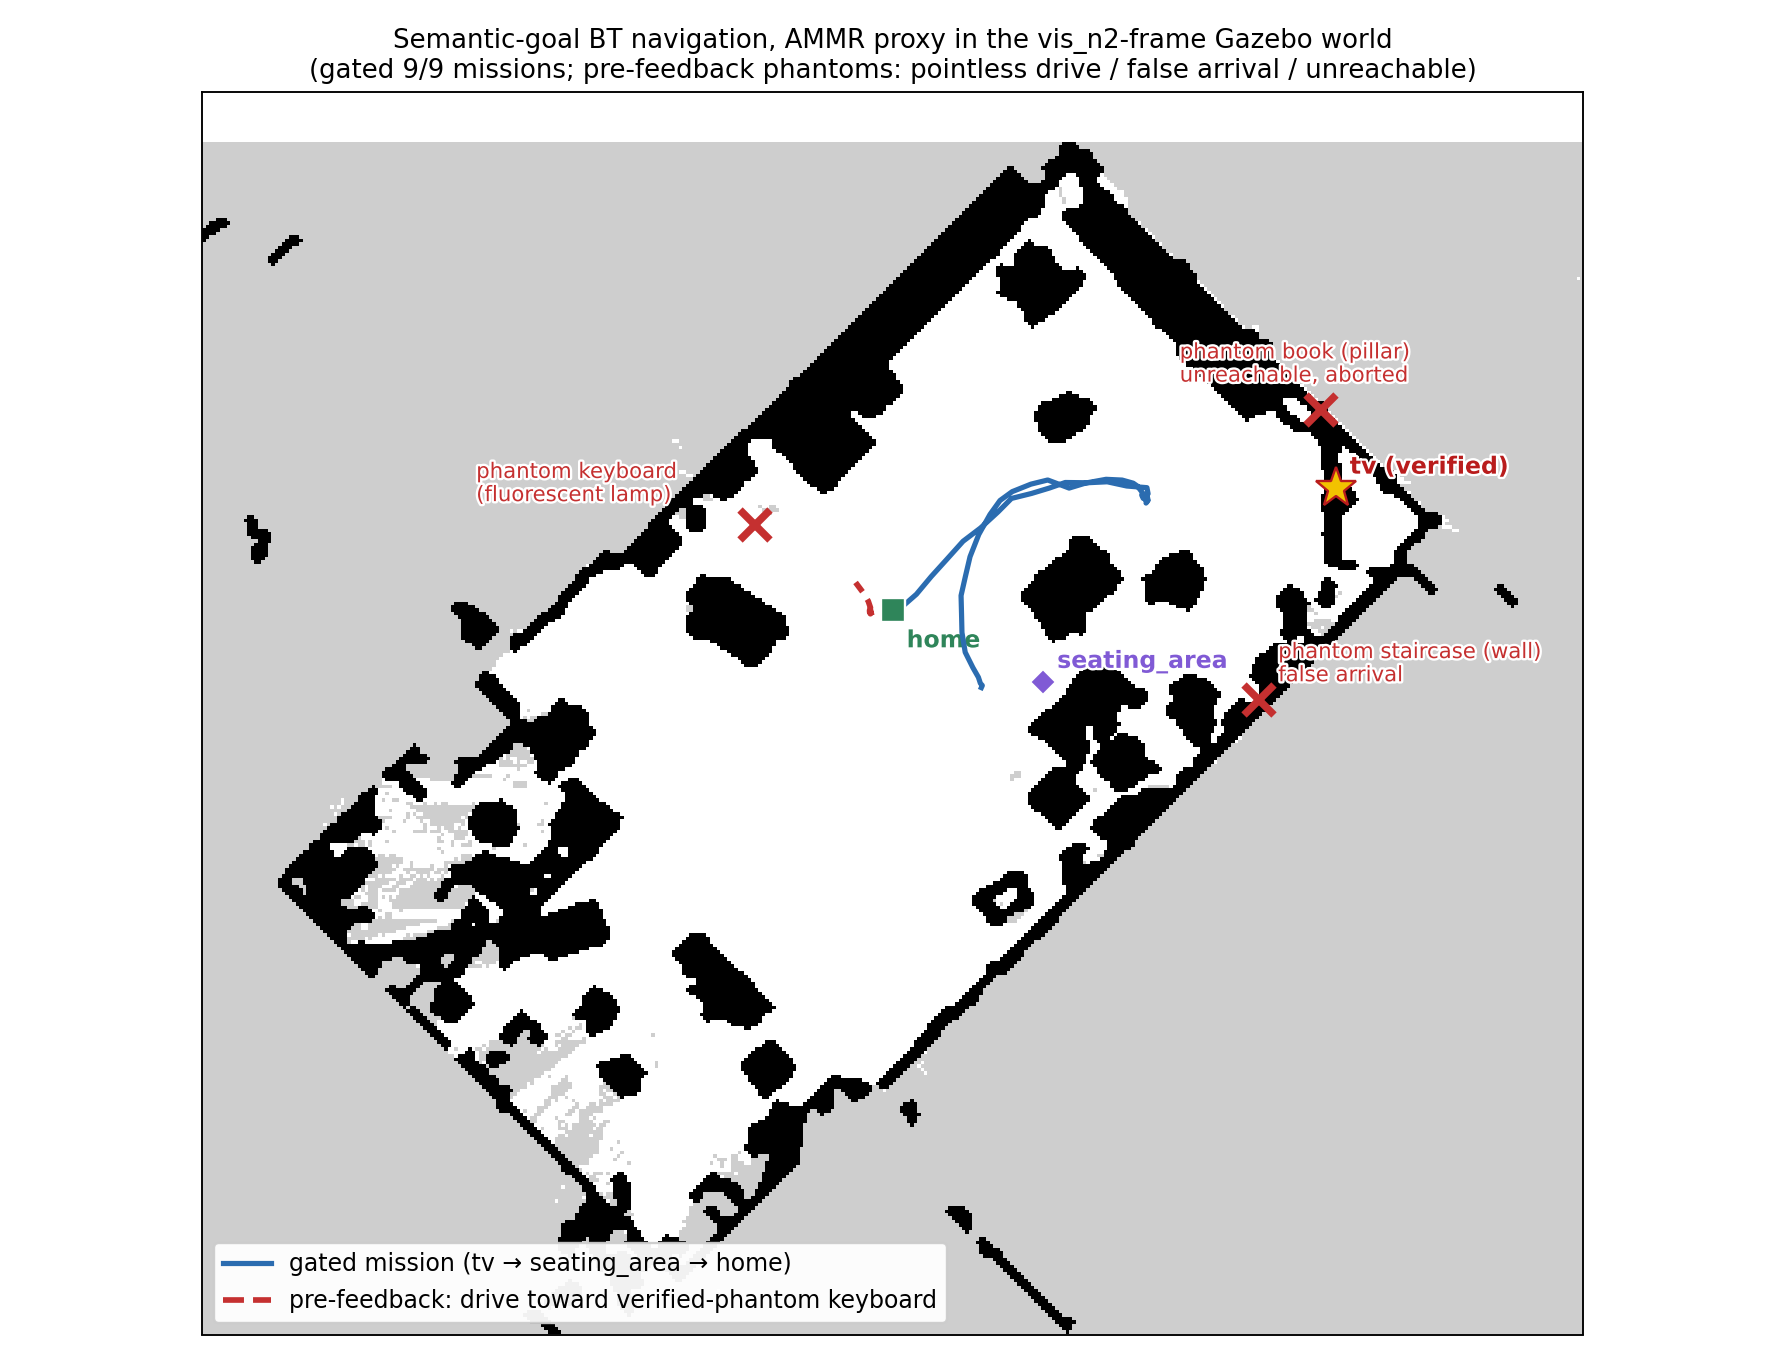
\includegraphics[width=0.8\linewidth]{figures/ele_fig15_semantic_nav_run.png}
\caption{Semantic-goal navigation of the AMMR proxy in the Gazebo twin of the
test room. Blue: a gated three-mission run (TV $\rightarrow$ seating area
$\rightarrow$ home). Red dashed: against the pre-feedback graph the robot
drives toward a verified-phantom keyboard; crosses mark the three phantom goals
with their failure modes. All three are refused once structure filtering and
owner feedback are applied.}
\label{fig:semnav}
\end{figure}

\paragraph{Physical robot.}
The mission stack was run unchanged against the physical AMMR in the test
room (robot-hall configuration) through the bridge of
Section~\ref{sec:real-robot}, with the console, the Isaac Sim twin, and the
robot all served from the same knowledge graph. Three semantic drives
completed---two \texttt{goto\_object} approaches to the wall TV and one
\texttt{goto\_place} drive into the monitor workstation region, each
3.6--4.0~m from the start---in 14--22~s with arrival errors of 0.22--0.34~m
(mean 0.30~m) between the robot's localized pose and the resolved goal; a
place command issued while the robot already stood inside the region completed
without motion (0.11~m from the region goal). The gate behaved as in
simulation: \texttt{goto\_object keyboard}, the owner-refuted phantom of
Table~\ref{tab:semnav}, was refused by the mediator in under one second with
zero robot motion, twice (Table~\ref{tab:realrobot},
Figure~\ref{fig:realrobot}). Missions were issued one at a time from a standing
start. The exercise is a bounded validation---one room, one platform, three
completed drives---but it confirms that the graph that survives verification,
gating, and owner feedback is directly consumable by a real robot, and that the
twin, console, and robot stay consistent because they read one store.

\begin{table}[htbp]
\caption{Real-robot semantic missions on the AMMR (test room, 15 September
2026). Goals are resolved by the mediator in the scan frame; distance is
straight-line start-to-goal; arrival error is the localized-pose-to-goal
distance at mission completion. Source: \emph{Electronics}~\cite{kim2026electronics}.}
\label{tab:realrobot}
\centering
\footnotesize
\begin{tabularx}{\textwidth}{X l c c c X}
\toprule
\textbf{Command} & \textbf{Resolved goal (m)} & \textbf{Dist.} & \textbf{Time} & \textbf{Err.} & \textbf{Outcome} \\
\midrule
\texttt{goto\_object tv} & tv\_006 (3.09, 1.91) & 4.0~m & 14~s & 0.34~m & completed \\
\texttt{goto\_object tv} (Fig.~\ref{fig:realrobot}a) & tv\_006 (3.09, 1.91) & 3.6~m & 20.8~s & 0.33~m & completed \\
\texttt{goto\_place electrical\_ maintenance\_area} (Fig.~\ref{fig:realrobot}b) & region ($-$0.69, 3.81) & 3.9~m & 22.1~s & 0.22~m & completed \\
\texttt{goto\_place display\_ briefing\_area} & region (3.31, 1.76) & 0.1~m & $<$1~s & 0.11~m & completed (already inside) \\
\texttt{goto\_object keyboard} ($\times$2, phantom) & --- & --- & $<$1~s & --- & refused by gate, no motion \\
\bottomrule
\end{tabularx}
\end{table}

\begin{figure}[!htb]
\centering
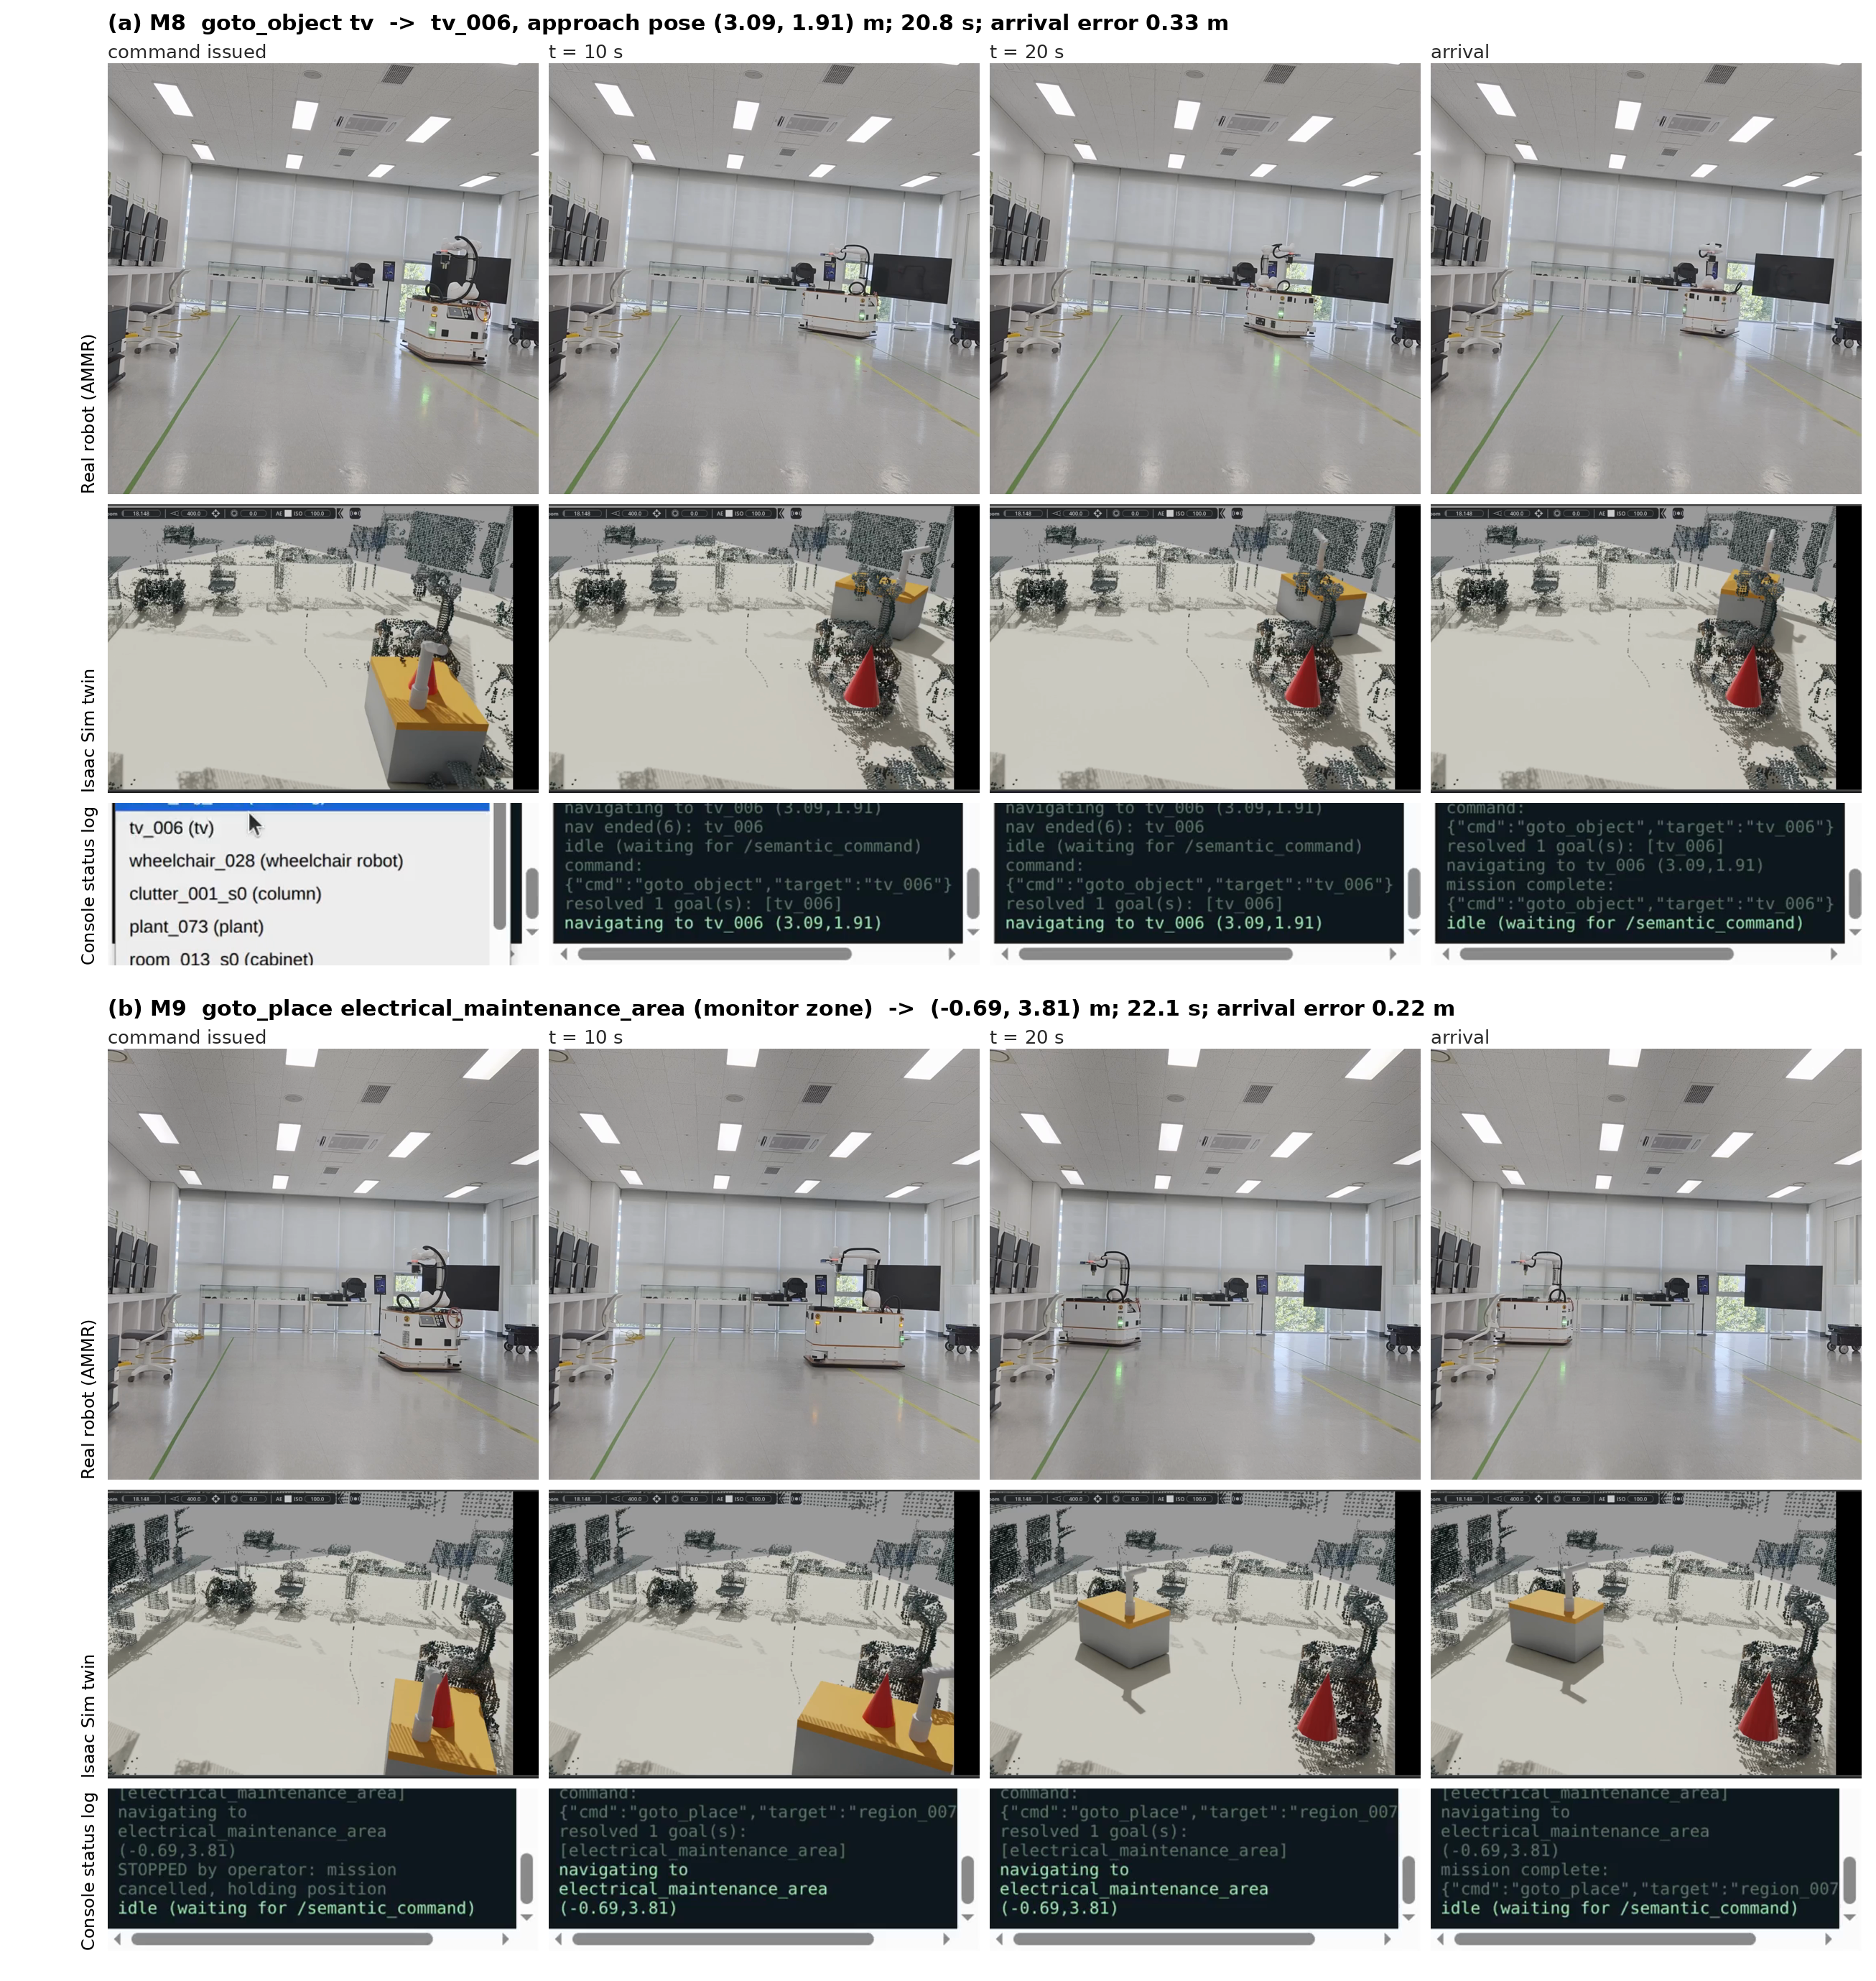
\includegraphics[width=\linewidth]{figures/ele_fig20_real_robot_missions.png}
\caption{Real-robot semantic missions (Table~\ref{tab:realrobot}). Rows: the
physical AMMR, the Isaac Sim twin derived from the same knowledge graph (the
red cone marks the twin's goal handle), and the management console's status
log; columns: command issued, 10~s, 20~s, and arrival. (a)~\texttt{goto\_object
tv}: the mediator resolves the verified node \texttt{tv\_006} to an approach
pose and the robot arrives 0.33~m from it in 20.8~s. (b)~\texttt{goto\_place
electrical\_maintenance\_area}: the region containing the monitor workstation,
reached in 22.1~s with 0.22~m error.}
\label{fig:realrobot}
\end{figure}

\section{Overhead Layer: Ceiling-Mounted Structure}
\label{sec:exp-overhead}

The overhead recognition pass of Section~\ref{sec:overhead} was run with its
parameters frozen on the two industrial epochs (T2, T3) and on the cafeteria
scene. Table~\ref{tab:overhead} summarizes the outcome of each stage and
Figure~\ref{fig:overhead} shows the T3 result over the floor-level graph.

\begin{table}[htbp]
\centering
\caption{Overhead recognition pass on three scenes (parameters frozen; the
verifier and protocol of Section~\ref{sec:exp-verify}). ``Cut'' = clusters
whose bottom lies at the band cut and are dropped as truncated continuations
of floor-level content; in-room = inside the room mask with the 0.5~m wall
tolerance.}
\label{tab:overhead}
\footnotesize\setstretch{1.15}
\begin{tabularx}{\textwidth}{X c c c}
\toprule
 & \textbf{Robot hall (T2)} & \textbf{Re-scan (T3)} & \textbf{Cafeteria} \\
\midrule
Reference cloud (points) & 989~K & 995~K & 546~K \\
Overhead-band points ($>$1.8~m) & 545~K & 512~K & 241~K \\
Ceiling levels found (m above floor) & 3.00 / 3.20 / 3.52 & 3.00 / 3.17 / 3.49 & 3.00 \\
Wall planes & 7 & 6 & 7 \\
Candidate points after ceiling/wall removal & 28.0~K & 39.6~K & 1.4~K \\
Floor-connected candidate points removed & 12.4~K & 31.4~K & 1.2~K \\
Clusters (after cut rule) & 18 & 12 & 0 \\
In-room objects & 5 & 6 & 0 \\
Verified unanimous / escalated / unverified & 1 / 4 / 0 & 1 / 3 / 2 & --- \\
VLM calls / cost & 57 / \$0.55 & 70 / \$0.67 & --- \\
\bottomrule
\end{tabularx}
\end{table}

\begin{figure}[!htb]
\centering
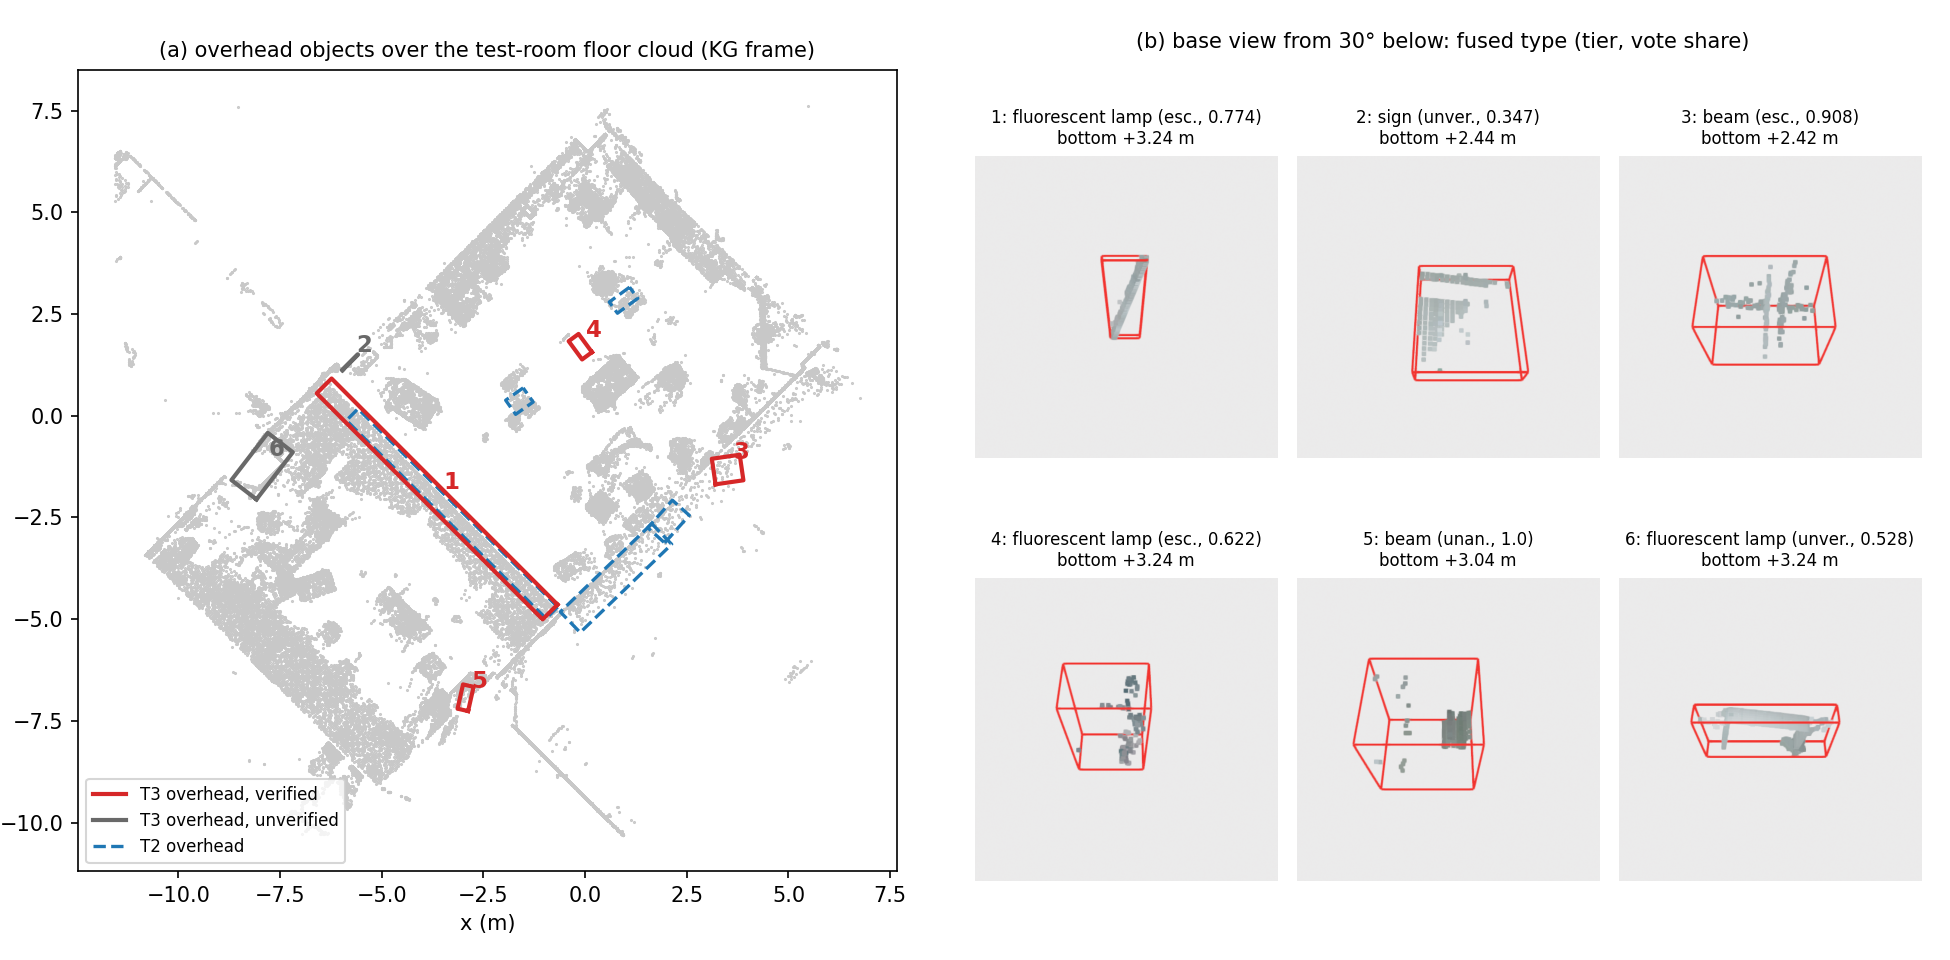
\includegraphics[width=\linewidth]{figures/fig6_overhead.png}
\caption{Overhead layer on the T3 epoch. (a)~The six in-room overhead objects
(red: verified tiers, gray: unverified) over the floor-level cloud, with the
five T2 overhead objects dashed in blue; (b)~each object's base render from
$30^\circ$ below with its fused type, tier, and vote share.}
\label{fig:overhead}
\end{figure}

\paragraph{What the pass finds.}
On T3 the pass isolates six in-room overhead objects: a 7.9~m lighting rail
0.25~m below the top ceiling level (verified as a fluorescent lamp by
escalation), three small fixtures at the same height (one verified
unanimously as a \emph{beam}, one as a fluorescent lamp by escalation, and
one left unverified with \emph{fluorescent lamp} at share 0.53), a hanging
thin plate 2.4~m above the floor (unverified; \emph{sign} at share 0.35),
and a sparse cross-shaped pipe junction (verified as \emph{beam} by
escalation). Every in-room object is attached to a ceiling level
(\emph{ceiling-hung}); the wall-mounted and suspended categories occur only
outside the room. Four of the six are verified (one unanimously, three by
escalation) and two remain unverified, at a cost of under \$1 for the scene.
On T2, the same room scanned from the
robot deck nine days earlier, the pass finds five in-room objects, all
verified (one unanimously, four by escalation). On the cafeteria the pass
finds \emph{nothing}: its single flat ceiling at 3.0~m carries recessed
lights that lie inside the ceiling band, and the 1.4~K candidate points that
survive ceiling and wall removal all belong to floor-connected clusters. A
null result on a scene that has no hanging structure is the intended
behavior of the pass, and it is reported as such.

\paragraph{Ground truth.}
\textcolor{red}{[Owner ground truth for the eleven T3 candidates (union of
the two extraction rules below) is being collected on the sheet
\texttt{overhead\_gt\_sheet.csv}; the precision figures of this paragraph
will be filled in from it.]} A render audit by the author, under the same
protocol as the floor-level audit, grades the lighting rail, the three
fixtures at the top level, the hanging plate, and the pipe junction as
plausible overhead objects; as for the floor pass, render-only annotation
cannot resolve fixture \emph{types} (a lamp housing and a cable tray look
alike from below at 3~cm spacing), so the type precision of the tiers is
reported only against the owner's inventory.

\paragraph{Extraction rule and its alternative.}
The frozen rule decides that a candidate is overhead by connectivity: a
cluster that reaches down into the driving band through the structure-free
lower cloud (at $\varepsilon=0.15$~m) is the upper part of a floor object. An
alternative rule, tested first, excludes candidate points that fall inside
the footprint of a floor-pass object beneath them; on T3 it returned nine
in-room candidates instead of six, because three fixtures that hang within
0.15~m of wall-mounted equipment (a projector-like bracket near the display
wall, a hanging rack, and a boxed unit) are absorbed by the connectivity
test, but on T2 it failed outright: the footprints of that epoch's merged
mega-clusters (Section~\ref{subsec:exp-params}) covered most of the room and
suppressed every fixture. Connectivity is therefore retained as the frozen
rule, and the owner sheet lists the union of both candidate sets so that
the recall cost of the connectivity rule can be scored.

\paragraph{Identity across epochs.}
Overhead objects are the most static content of a room, which makes them a
clean test of the identity policy of Section~\ref{sec:matching}. Upserting
the T2 set and then the T3 set into an overhead graph gives, for the T3
epoch, 0 matched, 1 moved, 5 inserted, and 4 absent. The reason is not
matching but coverage: the two scans see different parts of the ceiling. The
robot-deck exploration scan (T2) resolves the lighting rail and two fixtures
near the room center, whereas the six-setup re-scan (T3) resolves the rail
plus fixtures at the room's ends; only the rail is common to both, and its
centroid shifts by 0.52~m between the epochs because T2 captured 6.9~m of it
and T3 7.9~m---just outside the 0.5~m spatial gate, so the rail is
re-inserted under a new identity (the fragmentation error class of
Section~\ref{sec:exp-update}), and one same-type pair 1.9~m apart is
recorded as a false move. Two conclusions follow. First, ceiling coverage
depends on station placement at least as much as floor coverage does, so
the overhead layer inherits the coverage sensitivity of Part~A. Second,
elongated fixtures need an extent-overlap matching feature rather than a
centroid gate; this is the same feature the floor-level occlusion scenario
of Section~\ref{sec:exp-update} motivated, and it is left to future work.

\paragraph{Consumption.}
Verified overhead objects enter the knowledge graph with
\texttt{heightLevel = high}, their clearance below (2.4--3.2~m in the test
room), and their attachment, and the console and the Isaac Sim twin derive
them from the same store as every other node; a pointing or installation
task resolves against a verified overhead node exactly as a navigation task
resolves against a floor node, with the same gate refusing unverified ones.
No lifting platform executed such a task in this dissertation
(Chapter~\ref{ch:conclusion}).

\section{Summary against the Research Objectives}
\label{sec:exp-summary}

Table~\ref{tab:objsummary} maps the principal results of this chapter back to
the five research objectives of Section~\ref{sec:objectives} and states the
scope of each result.

\begin{table}[htbp]
\centering
\caption{Principal results against the research objectives, with scope.}
\label{tab:objsummary}
\small
\begin{tabularx}{\textwidth}{l X X}
\toprule
\textbf{Obj.} & \textbf{Principal result} & \textbf{Scope} \\
\midrule
O1 & Visibility rule: LOS $77\%\to84$--$85\%$ (paired ablation, $+1$--2 scans); on hardware $77.6\to92.1\%$; all visibility runs register at 4--5~mm bundle error, 84--88\% overlap & Room-scale indoor, 2D visibility, one scanner, one test room \\
O2 & Byte-identical backbone across hosts; recall 0.952 vs.\ owner inventory at the operating point; learned closed-set/projection baselines fail on industrial content & Proxy metrics for baseline screening; one industrial scene \\
O3 & Escalation $77.8\to88.9\%$ / $78.1\to84.4\%$; unanimity 94--100\% precision; gated query 83.3\% with 3/4 traps blocked; zero identity switches over three epochs; re-verification at 3.1\% of rebuild; automated recall $28\to85\%$ & One building; tier precision is scene-scoped (cafeteria 35--60\%); replay on development scene \\
O4 & Scan-to-sim in 78.5~s; RTF 5.6 physics-only, 104~FPS viewport; dimensions within 2\%; end-to-end positioning 5.5~cm MAE; overhead layer: 6 in-room ceiling objects on T3 (5 verified), null result on the flat-ceiling cafeteria & One room; overhead band validated at the representation level, not with a lift \\
O5 & Simulator-issued goals 4/4 (0.21~m); console-issued semantic missions 3 completed (0.30~m mean error), 2 phantom refusals with zero motion; twin, console, robot consistent from one store & One platform (AMMR), missions from a standing start \\
\bottomrule
\end{tabularx}
\end{table}

